\section{Контрольні питання}


\bigskip


\bigskip

\liststyleWWviiiNumxlv
\begin{enumerate}
\item Чим відрізняються процедури зашифрування та розшифрування?
\item Як визначається поняття теоретичної та практичної стійкості криптосистеми?
\item Сформулюйте правило Керкгоффса.
\item Які припущення зробив Шеннон у запропонованій ним моделі випадкового
шифру?
\item Наведіть означення цілком таємної системи в теорії Шеннона.
\item Що таке границя Шеннона?
\item Чи виконання нерівності Шеннона є достатньою умовою для цілковитої
таємності?
\item Чи існують цілком таємні криптосистеми? 
\end{enumerate}

\bigskip


\bigskip


\bigskip

 $ $\textbf{ ЛЕКЦІЯ  4}


\bigskip

{\centering\bfseries
НЕНАДІЙНІСТЬ  КЛЮЧА  І  ВІДКРИТОГО  ТЕКСТУ.
\par}

{\centering\bfseries
 ВІДСТАНЬ  ОДНОЗНАЧНОСТІ
\par}


\bigskip


\bigskip

Для цілком таємної криптосистеми неможливо з криптограми здобути будь-яку
інформацію щодо відкритого тексту. Якщо ж криптосистема не є цілком таємною (а
більшість криптосистем, що використовуються на практиці, саме такі), то за
криптограмою  можна отримати певну інформацію про текст, що був зашифрований,
про таємний ключ, а можливо повністю зламати шифр --- знайти таємний ключ і
відкритий текст. Розглянемо ці питання докладніше.


\bigskip

\textit{Означення4.1}.  \textit{Ненадійністю ключа }називається  величина 

$$

\textit{Означення4.2}\textit{. Ненадійністю відкритого }\textit{тексту}
називається  величина 

$$

Тобто  криптограма  містить у середньому $I$\textit{
}\textbf{(}\MessagesSet\textbf{,}\CryptogramsSet\textbf{)}=\textit{
$H$\textbf{(}\MessagesSet\textbf{) -
$H$(\MessagesSet\textbf{/}\CryptogramsSet\textbf{)}\textbf{  }біт\textbf{
}інформації відносно ВТ (у цілком таємної криптосистеми така інформація
дорівнює нулю) і  $I$\textit{
}\textbf{(}\textbf{K}\textbf{,}\CryptogramsSet\textbf{)}=\textit{
$H$\textbf{(}\textbf{K}\textbf{)-}\textit{
$H$\textbf{(}\textbf{K}\textbf{/}\CryptogramsSet\textbf{)}\textbf{ }біт
інформації щодо ключа. 

\textit{ТЕОРЕМА 4.1}Нехай в моделі криптосистеми за Шенноном  ( див.
лекцію \textbf{3})  ключ вибирається незалежно від ВТ. Тоді для ненадійності 
ключа буде виконуватись рівність  

$$H$(\textbf{K}\textbf{/}\CryptogramsSet) =  $H$(\MessagesSet) +
$$

{\itshape
Доведення }

Згідноз властивостями умовної ентропії 

$H$\textbf{(}\MessagesSet\textbf{,}\textbf{K}\textbf{,}\CryptogramsSet\textbf{)
= $H$\textbf{(}\MessagesSet\textbf{,}\textbf{K}\textbf{) }\textit{+
$H$\textbf{(}\CryptogramsSet\textbf{/}\MessagesSet\textbf{,}\textbf{K}\textbf{)
= $H$\textbf{(}\textbf{K}\textbf{,}\CryptogramsSet\textbf{) }\textit{+
$H$\textit{(}\MessagesSet\textbf{/}\textbf{K}\textbf{,}\CryptogramsSet\textbf{).
}

\textbf{О}скільки через однозначність шифрування та розшифрування 
$H$\textbf{(}\CryptogramsSet\textbf{/}\MessagesSet\textbf{,}\textbf{K}\textbf{)
=$H$\textbf{(}\MessagesSet\textbf{/}\textbf{K}\textbf{,}\CryptogramsSet\textbf{)=}0\textbf{,
}то\textbf{
$H$\textbf{(}\textbf{K}\textbf{,}\CryptogramsSet\textbf{)=$H$\textbf{(}\MessagesSet\textbf{,}\textbf{K}\textbf{)}\textbf{.}\textbf{
}

Далі, враховуючи незалежність ключів і ВТ, отримуємо  \textbf{ }

$H$\textbf{(}\MessagesSet\textbf{,}\textbf{K}\textbf{) =
$H$\textbf{(}\MessagesSet\textbf{) +
$H$\textbf{(}\textbf{K}\textbf{) } $\Rightarrow $\textit{
$H$\textbf{(}\textbf{K}\textbf{,}\CryptogramsSet\textbf{) =
$H$\textbf{(}\MessagesSet\textbf{) +
$H$\textbf{(}\textbf{K}\textbf{)}. З іншого боку

$H$\textbf{(}\textbf{K}\textbf{,}\CryptogramsSet\textbf{) }\textit{=
$H$\textbf{(}\CryptogramsSet\textbf{) +
$H$\textbf{(}\textbf{K}\textbf{/}\CryptogramsSet\textbf{) } $\Rightarrow
$\textbf{ $H$\textbf{(}\textbf{K}\textbf{/}\CryptogramsSet\textbf{) =
$H$\textbf{(}\MessagesSet\textbf{) +
$H$\textbf{(}\textbf{K}\textbf{) ---
$H$\textbf{(}\CryptogramsSet\textbf{)}.\textbf{ }Теорема\textbf{ }доведена.

Розглянемо модель Шеннона  криптосистеми  з незалежними  від відкритого тексту
ключами, в якої ВТ і ШТ --- це послідовності довжини  $n$
символів з алфавіту   $Z_m$,  $n$ $?$\textit{
}\textbf{$N$}\textit{.}  Причому,  ВТ --- розумний текст з середньою
інформацією на символ  $H_\infty$.  Позначимо  через   $ $   $ $ $ $ $ $
 \textbf{K}(C) =   $\left\{\;k\in K:\exists
M,\;E_k\right.(M)=C\left.\right\}$

множину ключів, при шифруванні на яких  може бути отримано ШТ  \textit{С} (для
деяких повідомлень). Для фіксованого ШТ  \textit{С}  число хибних ключів
дорівнює   $|K(C)|-1$. Середнє число хибних ключів 


\bigskip

$$k$ $_n$ =   $\sum_{C\in C}{\probability{C}\cdot (|K(C)|-1)$
=   $$


\bigskip

\textit{ТЕОРЕМА 4.2}Для будь-якого шифру   $\sum {$ з незалежними
від ВТ ключами  при достатньо великих $n$ виконується  нерівність 

$$k$ $_n$   $?$  
$$


\bigskip

 де  $R$  {}-  надлишковість  ВТ, що при достатньо великих $n$
дорівнює надлишковості мови ВТ (див. лекцію 2).

{\itshape
Доведення }

 Для  достатньо великих  $n$ 

{\centering\bfseries
 $\entropy{$ M} $?n \cdot H_{{\infty
}}=n \cdot H}}_0(1-R)=n(\log_2m)(1-R)\text{.$$

Очевидно \textit{ $H$(\CryptogramsSet)  $?$  log $_{{2$
$|С}|$ =  $n$ log $_{{2$ $m$\textit{.  З останніх
двох співвідношень та теореми 4.1  отримуємо:

$$H$(\textbf{K}\textbf{/}\CryptogramsSet) = $H$(\MessagesSet) +
$H$\textit{(}\textbf{K}) --- $H$(\CryptogramsSet)  $?$ 
$H$(\textbf{K}) + $n$ (log $_2$ $m$)
(1-$$

$$--- $H$(\CryptogramsSet)  $?$ $H$\textit{(}\textbf{K}) +
$n$(1-$R$) log $_2$ $m$ --- $n$ log
$_2$ $m$ = $H$(\textbf{K}) --- $nR$ log $_{{2$
$$

Таким чином, 

$$H$(\textbf{K}\textbf{/}\CryptogramsSet) $?$\textit{ $H$(\textbf{K})
--- $$

З іншого боку маємо:

$$H$(\textbf{K}\textbf{/}\CryptogramsSet) =   $\sum_{C\in C}{$
$P$(C) $H$(\textbf{K}/$C$)  $?$  $\underset{{C\in
C}}{\sum }{}$$

Далі за нерівністю Ієнсена

$$H$(\textbf{K}\textbf{/}\CryptogramsSet)   $?$ log $_{{2$(
$\sum_{C\in C}{}$ $P$($C$\textbf{) } $|K(C)|$ = 
log $$

Враховуючи обидві отримані нерівності для 
$H$(\textbf{K}\textbf{/}\CryptogramsSet) можемо тепер записати таку
нерівність 

$$H$(\textbf{K}) --- $n$\textit{ $R$ log $_2$
$$

Звідки  маємо

$$log  $\frac{2^{\entropy{K}}}{m^{nR}}$   $?$  log
($$

І  далі отримуємо твердження теореми 4.2:  $k$ $_n$   $?$  
$\frac{2^{\entropy{K}}}{m^{nR}$  --- 1. 

Нехай 
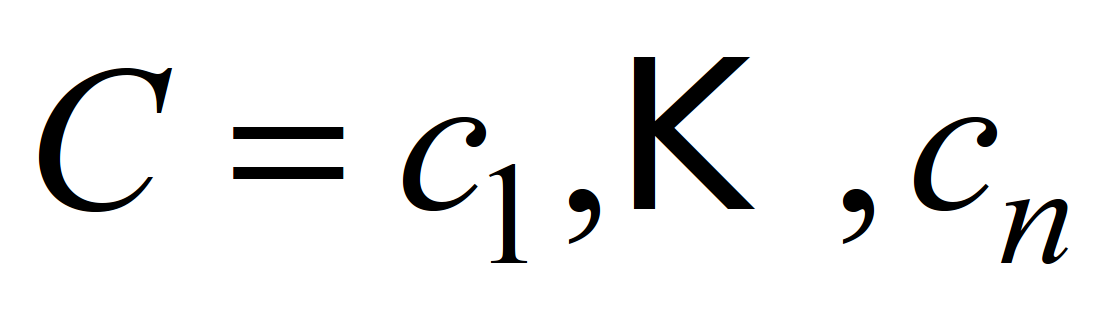
\includegraphics[width=1.1764in,height=0.3327in]{crypt-img/crypt-img38.png} ,  
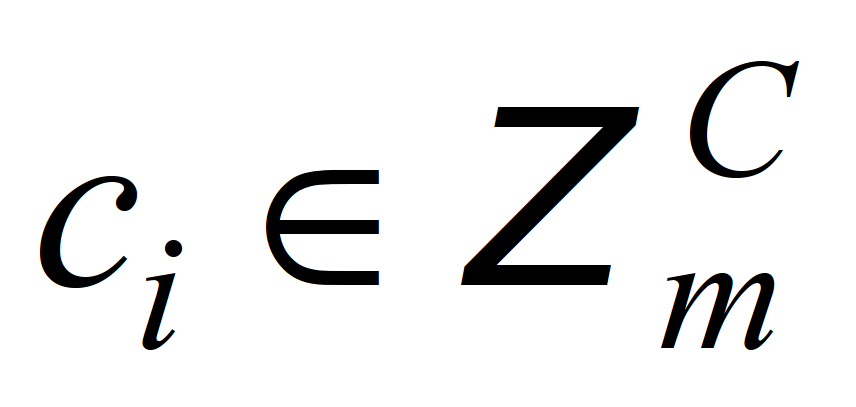
\includegraphics[width=0.7201in,height=0.3472in]{crypt-img/crypt-img39.png} , ---
деяка криптограма, 
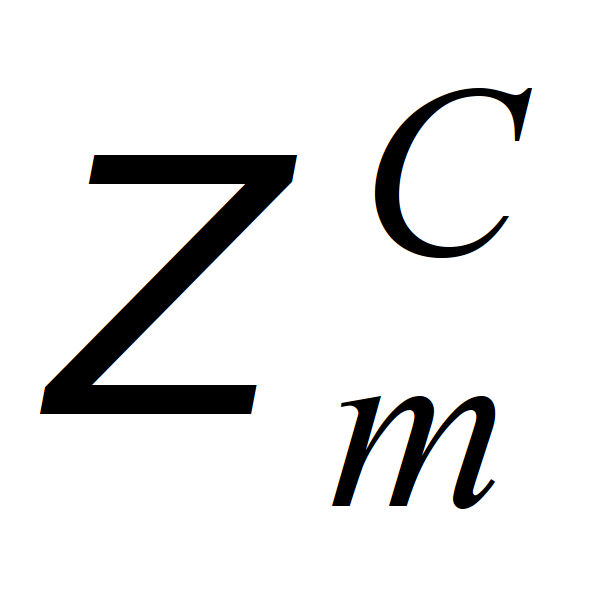
\includegraphics[width=0.3465in,height=0.3465in]{crypt-img/crypt-img40.png}  ---
алфавіт криптограм.

\textit{Означення 4.3}. \textit{Функцією ненадійності ключа} називається 
функція 

{\centering 
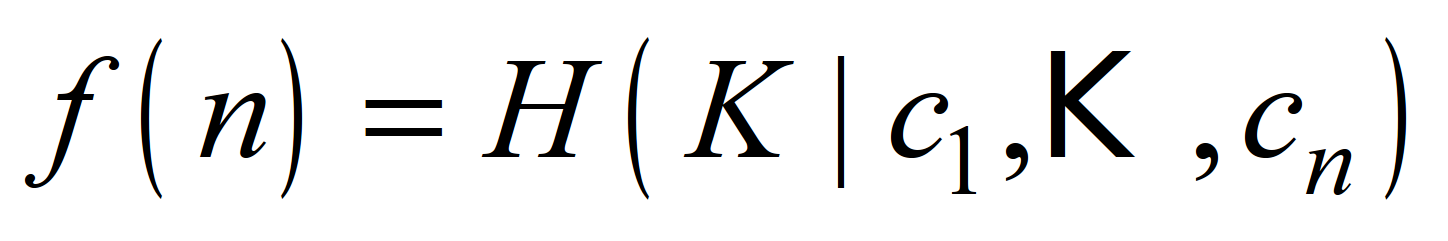
\includegraphics[width=1.9882in,height=0.3346in]{crypt-img/crypt-img41.png}
\par}

(ентропія ключа за умови, що відомо \textit{n }символів криптограми).

Очевидно, що 
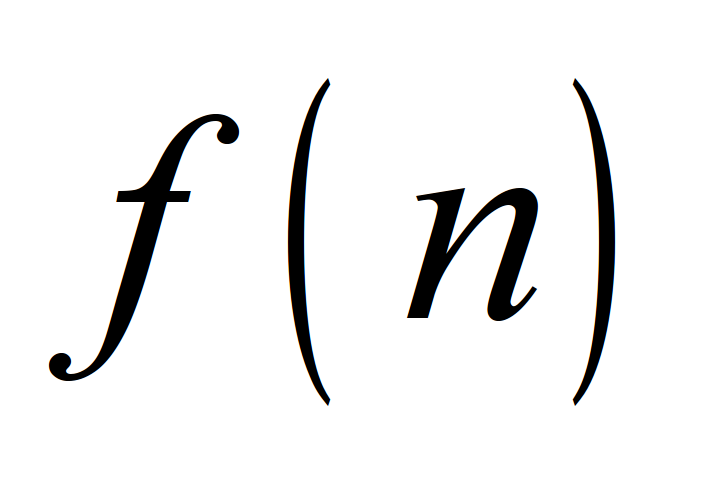
\includegraphics[width=0.4874in,height=0.3354in]{crypt-img/crypt-img42.png}  ---
незростаюча функція, а саме:

$$ 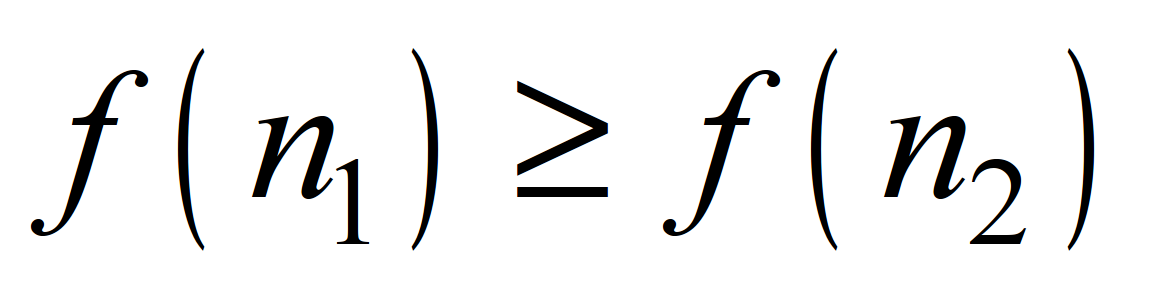
\includegraphics[width=1.2555in,height=0.3339in]{crypt-img/crypt-img43.png} , 
коли  
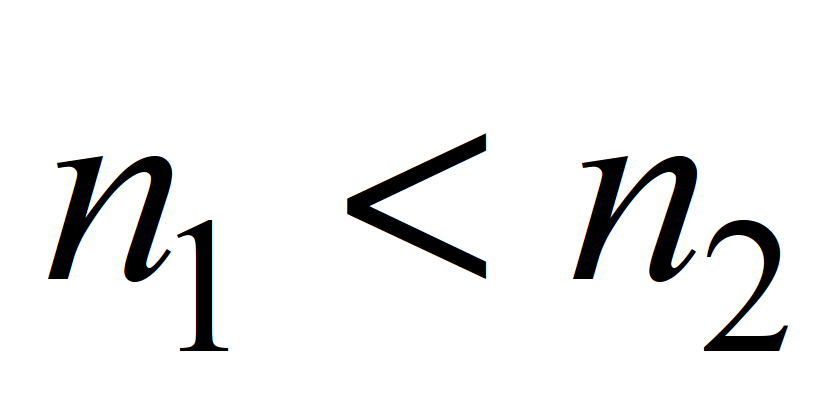
\includegraphics[width=0.598in,height=0.2984in]{crypt-img/crypt-img44.png} .
\par}

\textit{Означення4.4}. \textit{Відстанню  однозначності} називається
величина $u$= min 
$\left\{\;n|k_n\right.=0\left.\right\$

Тобто  за криптограмою довжиною більшою, ніж відстань однозначності,
криптоаналітик в принципі може знайти таємний ключ, що використовувався при
зашифруванні, оскільки його невизначеність дорівнює нулю. Але, як ми побачимо в
наступних лекціях, це не завжди можливо через  велику трудомісткість необхідних
обчислень. Зауважимо, що відстань однозначності --- це усереднена за ключами та
криптограмами (а отже і відкритими текстами) характеристика.

\textit{ТЕОРЕМА 4.3 } Для будь-якого шифру   $\sum {$ з незалежними від ВТ 
ключами  при достатньо великих $n$ виконується  співвідношення

$$

{\itshape
Доведення}

 Таємний ключ може бути однозначно знайдений за  криптограмою, якщо число хибних
ключів дорівнює нулю. Тобто, з урахуванням усереднення за ключами і
криптограмами, це означає, що\textit{  $k$ $_n$=0. Далі з
теореми 4.2 отримаємо: 

$$1   $?$   $\frac{2^{\entropy{K}}}{m^{nR}$  
$\Rightarrow $\textit{  $n$\textit{ $R$log
$$


\bigskip

Звідки  випливає, що  $n$  $?$  $H$(\textbf{K}) / $R$ log
$m$\textit{.}З останньої нерівності видно, що мінімальне
$n$, для якого середнє число хибних ключів дорівнює нулю, задається
формулою для відстані однозначності, що наведена у формулюванні теореми.   $ $
$ $ 

Формула Шеннона для відстані однозначності добре погоджується з криптографічною
практикою при достатній довжині криптограми  і у більш загальних випадках

{\itshape
 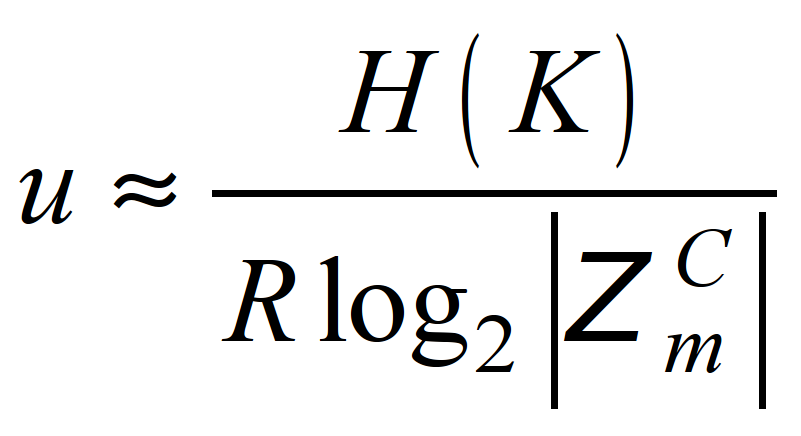
\includegraphics[width=1.3335in,height=0.7189in]{crypt-img/crypt-img45.png} ,}

де $R$--- надлишковість криптограми,  

$$

Запис 
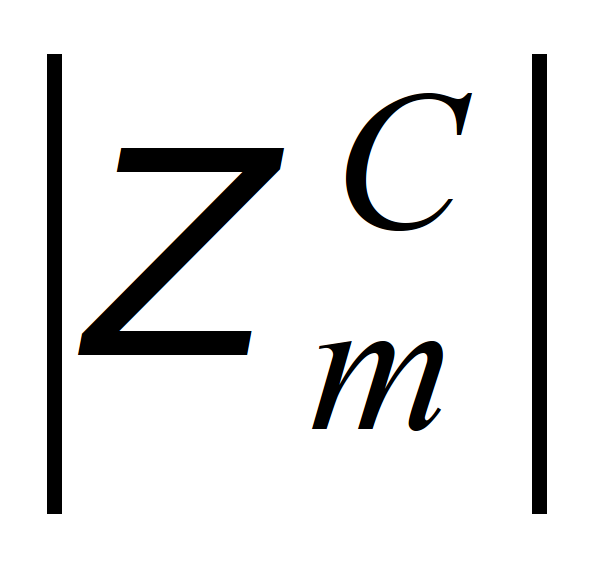
\includegraphics[width=0.4374in,height=0.4063in]{crypt-img/crypt-img47.png} 
означає число символів алфавіту криптограми, а $n$ --- її довжина. 

\textbf{\textit{Зауваження}}\textbf{.} Яку довжину криптограми в теоремах 4.2 і
4.3 можна вважати достатньою при практичному застосуванні? Це визначається
точністю співвідношення  $H$(\MessagesSet)  $?$\textit{  $n \cdot H$
$_\infty$. Як ми бачили в лекції 2, при $n$ біль-шому за 30 ця
приблизна рівність стає практично точною. Для $n$меншого 10 у
наведеному вигляді формула для відстані однозначності дає значну помилку у бік
зменшення відстані однозначності. Щоб скоректувати у такому разі відповідь
треба враховувати відповідне зменшення надлишковості $R$ при невеликих
довжинах криптограм.

\textit{Наслідок формули Шеннона}. Якщо алфавіт шифрованого тексту співпадає з
алфавітом відкритого тексту (
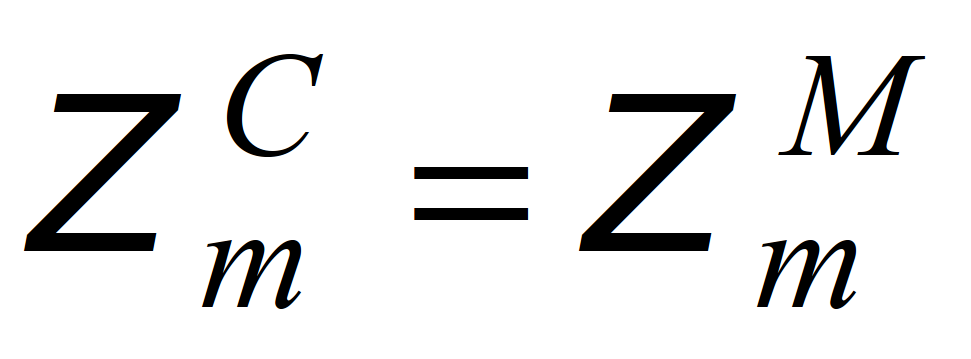
\includegraphics[width=0.9016in,height=0.3339in]{crypt-img/crypt-img48.png} ),
то надлишковість криптограми співпадає з надлишковістю відкритого тексту
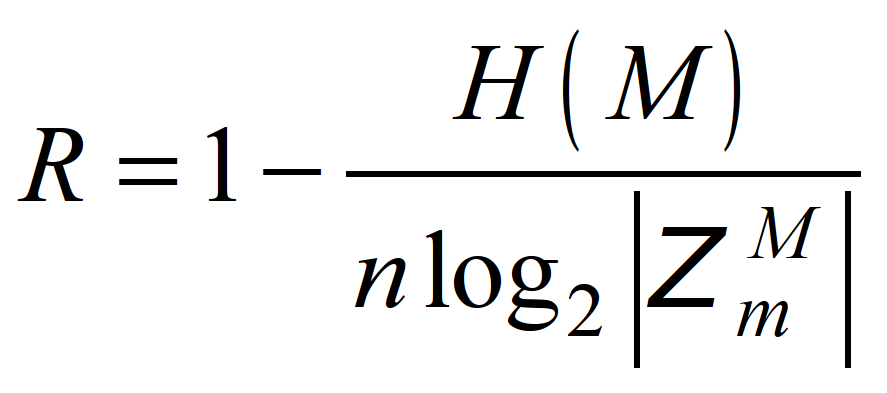
\includegraphics[width=1.6252in,height=0.7075in]{crypt-img/crypt-img49.png} . 
Як зазначалося у лекції 2, для iндоєвропейських мов надлишковість мови 
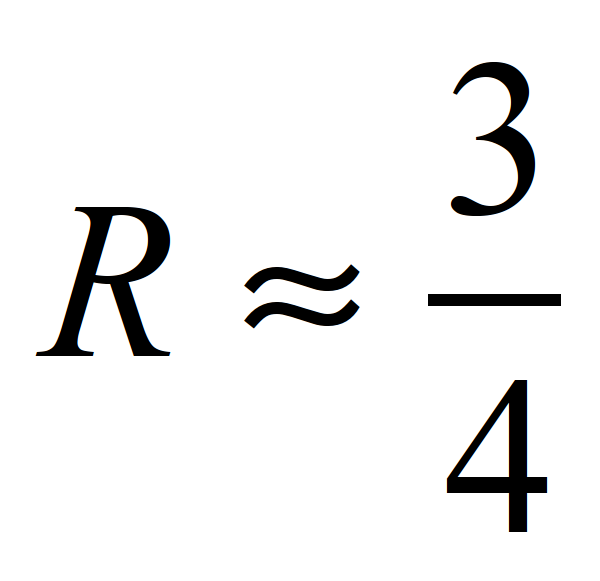
\includegraphics[width=0.5516in,height=0.5209in]{crypt-img/crypt-img50.png}   
(60-80\% залежно від тексту ).

Надлишковість в бітах на знак алфавіту 
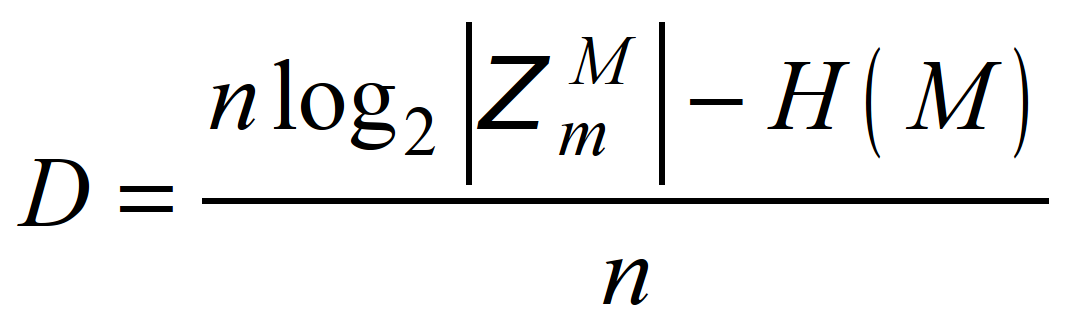
\includegraphics[width=2.122in,height=0.65in]{crypt-img/crypt-img51.png} . Якщо
  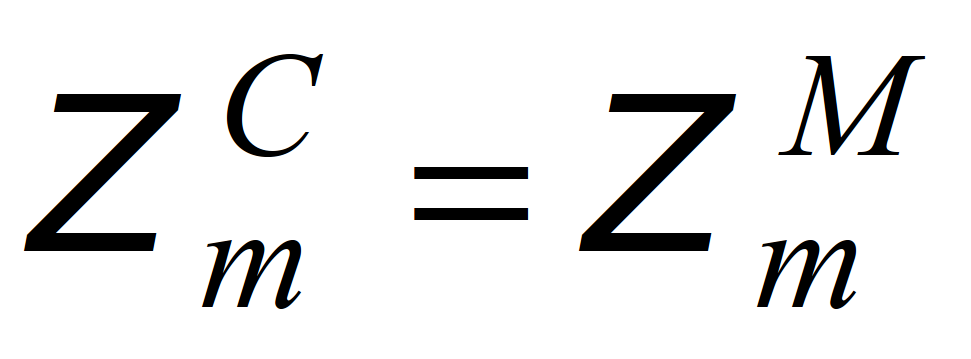
\includegraphics[width=0.9047in,height=0.3311in]{crypt-img/crypt-img52.png} ,
 то   $u\approx \frac{\entropy{K}}{D$.  Коли до того ж алфавіт ключа співпадає з
алфавітом шифрованого і відкритого текстів, а розподіл ключів  рівноймовірний,
то  
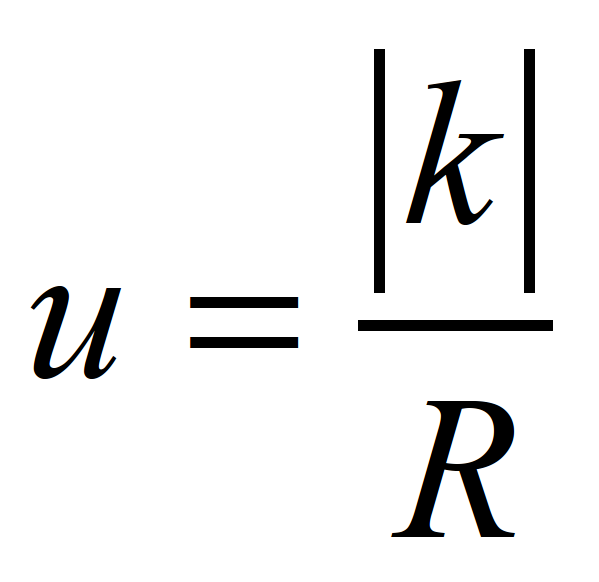
\includegraphics[width=0.5862in,height=0.5665in]{crypt-img/crypt-img53.png} , 
де  
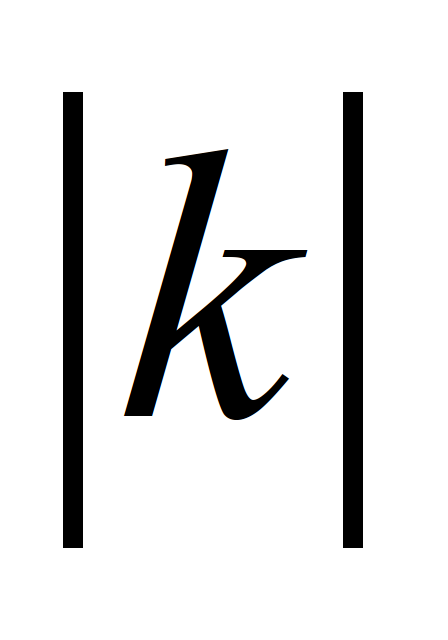
\includegraphics[width=0.2291in,height=0.3335in]{crypt-img/crypt-img54.png}  ---
довжина ключа в символах алфавіту.

\textbf{\textit{Зауваження}}\textbf{.} Якщо при криптоаналізі використовуються
не всі статистичні та функціональні залежності мови, то надлишковість
$R$у формулі для відстані однозначності треба брати меншою.
Так, якщо при криптоаналізі використовується тільки частота букв, то
надлишковість має бути як у моделі відкритого тексту М1 (дивись лекцію 2),
тобто $R$=0.13 --- 0.15  і відстань однозначності  збільшиться в декілька
разів.  Очевидно, коли  $R$ $\rightarrow $ 0,\textit{  u}
$\rightarrow \infty $\textit{.  }Нагадаємо, що відстань однозначності --- це
усереднена за ключами і криптограмами достатньої  довжини характеристика. 
истовується тільки частота букв, то надлишковіссть має бути як

Поняття відстані однозначності дає орієнтир: чи можливо досягти успіху в повному
зламі криптосистеми за криптограмою певної довжини, чи ні.


\bigskip


\bigskip

\section{Контрольні питання}


\bigskip


\bigskip

\liststyleWWviiiNumx
\begin{enumerate}
\item Чи може бути зламана цілком таємна криптосистема по зашифрованому тексту
певної довжини?
\item Наведіть означення ненадійності ключа та ненадійності відкритого тексту.
Який зміст вкладається в ці поняття з точки зору теорії інформації?
\item Що таке функція ненадійності ключа?
\item Якою повинна бути ненадійність ключа, щоб його можна було знайти по
криптограмі, якщо виконати певний обсяг обчислень?
\item Що таке відстань однозначності?
\item Як впливає надлишковість на відстань однозначності?
\item В якому розумінні відстань однозначності є усередненою характеристикою?
\item Яка відстань однозначності у цілком таємної криптосистеми? 
\end{enumerate}

\bigskip


\bigskip


\bigskip

{\bfseries
ЛЕКЦІЯ  5}


\bigskip

{\centering\bfseries
МОНОАЛФАВІТНІ  ПІДСТАНОВКИ
\par}


\bigskip


\bigskip

\section{Підстановки на алфавіті. Підстановка як криптографічне перетворення}


\bigskip


\bigskip

Нехай $Z$\textit{\textsubscript{m}} =
\{$z$\textsubscript{1},$z$\textsubscript{2},…$z$\textit{\textsubscript{m}}\}
--- алфавіт відкритого та шифрованого текстів.

\begin{definition}
\textit{ Підстановкою на алфавіті}\textbf{\textit{
}}\textbf{$Z$}\textbf{\textit{\textsubscript{m}}} називається
взаємно-однозначне відображення  $\pi :Z_m\rightarrow Z_m$.

Інакше кажучи, будь-яка перестановка елементів
$Z$\textit{\textsubscript{m}}\textsubscript{ } визначає підстановку на
$Z$\textit{\textsubscript{m}}\textsubscript{ }. На множині підстановок
на $Z$\textit{\textsubscript{m}} можна визначити операцію множення 
$\pi _1\cdot \pi _2$ (композиція підстановок).

З курсу дискретної математики вам відомо, що множина підстановок на
$Z$\textit{\textsubscript{m}}\textsubscript{ } утворює групу відносно
операції множення. Одиницею цієї групи є тотожна підстановка; для кожної
підстановки \textit{\textgreek{p}}\textbf{ } існує обернена підстановка
\textit{\textgreek{p}}\textsuperscript{{}-1} :
\textit{\textgreek{p}}\textsf{}\textit{\textgreek{p}}
\textsuperscript{{}-1}\textbf{ = }1. Ця група називається симетричною і
позначається SYM\textbf{($Z$\textit{\textsubscript{m}}\textbf{)}.
Кількість всіх підстановок на
$Z$\textit{\textsubscript{m}}\textsubscript{ } дорівнює
$m$\textit{!}.

Якщо задана підстановка \textbf{\textit{\textgreek{p}}}\textbf{} на
$Z$\textit{\textsubscript{m}}\textsubscript{ }, то можна згідно з нею
букві ВТ  співставити букву ШТ. Але криптографічне перетворення повинно
задавати правило шифрування тексту будь-якої довжини $n$.

Позначимо  $Z_m^n$ множину $n$-грам над алфавітом
$Z$\textit{\textsubscript{m}}.

\textit{Означення 5.1.}\textit{ Криптографічним перетворенням Т }називається
сімейство перетворень  $T=\;\{T^{(n)},\;n=1,2,\dots\$,
де  $T^{(n)}:\;Z_m^n \to \;Z_m^n$\textsf{.}

\textit{Означення 5.2.}\textit{ Підстановка}\textbf{}(як
криптосистема) --- це криптографічне перетворення \textit{Т}\textbf{},
де  $T^{(n)}=\{\pi _1,\pi _2,\dots,\pi
_n\}$.

Тобто при шифруванні шифром підстановки тексту довжини $n$ перша буква ШТ
одержується з першої букви ВТ за допомогою підстановки на алфавіті
\textit{\textgreek{p}}\textsubscript{1}, друга --- за допомогою
\textit{\textgreek{p}}\textsubscript{2 }, ..., остання --- за допомогою
\textit{\textgreek{p}}\textit{\textsubscriptn}.

Таким чином, криптографічне перетворення \textit{Т} задається ключем  $k=\{\pi
_1,\pi _2,\dots\}$- нескінченною послідовністю
підстановок. Звернемо увагу на те, що букви при підстановці шифруються
незалежно одна від одної і кожна, взагалі кажучи, своєю підстановкою.

\textit{Означення 5.3.}Підстановка називається
\textit{моноалфавітною}, якщо\textbf{
}\textit{\textgreek{p}}\textit{\textsubscript{і}} =\textsf{\textit{
}}\textit{\textgreek{p}}\textbf{ , }\textit{і=1,2,...} (тобто всі букви
шифруються тією ж самою підстановкою). Якщо ж у послідовності   $\{\pi
_1,\pi _2,\dots\}$ не всі підстановки однакові, то
таке криптографічне перетворення називається \textit{поліалфавітною}
підстановкою.

Моноалфавітну підстановку ще називають \textit{шифром простої заміни}.

Підкреслимо, що при моноалфавітній підстановці одна й та сама буква алфавіту, що
зустрічається у ВТ, шифрується тією ж самою буквою ШТ незалежно від її місця у
тексті. Наприклад, якщо підстановка \textbf{\textit{\textgreek{p}}} переводить
букву ,,а'' в  букву ,,м'', то де б не зустрілась буква ,,а'' у ВТ, вона буде
зашифрована як ,,м''. У разі ж поліалфавітної підстановки одна й та сама буква
алфавіту може шифруватись по-різному в залежності від її місця у ВТ.


\bigskip


\bigskip

\section{Шифр Цезаря}


\bigskip


\bigskip

Найпростіша моноалфавітна підстановка --- це шифр Цезаря. Ототожнимо букви
алфавіту $Z$\textit{\textsubscript{m}} з числами від\textbf{ }0 до
\textit{m-}1 і позначимо через $x$ довільну букву ВТ, а через $y$
--- відповідну букву ШТ. Тоді в шифрі Цезаря   $y=x+b\;(mod\;m)$, де 
$0\le b\le m-1$ --- ключ (сам Цезар використовував ключ $b$\textit{=}3).
В цьому випадку підстановка на алфавіті  $\pi $ є циклічним зсувом алфавіту
на  $b$ позицій вправо.

Для того, щоб знайти ключ, маючи лише ШТ, знайдемо
$y$\textbf{\textit{\textsuperscript{*}}} - букву, що найчастіше
зустрічається у ШТ. Нехай $x$\textbf{\textit{\textsuperscript{*}}} ---
буква алфавіту, що має найбільшу частоту у мові, якою написаний ВТ. Тоді, якщо
текст достатньо довгий, щоб у ньому проявилися закономірності мови,
найвірогідніше, що $x$\textbf{\textit{\textsuperscript{*}}} зашифровано
у  $y$\textbf{\textit{\textsuperscript{*}}}. Отже, маємо 
$y^{?}=x^{?}+b\;(mod\;m)$, звідки ключ 
$b=y^{?}-x^{?}(mod\;m)$.

Звичайно, існує деяка імовірність помилки при виборі образу
$x$\textbf{\textit{\textsuperscript{*}}}, а отже, і при визначенні ключа
 $b$. Тоді потрібно взяти другу за частотою букву ШТ
$y$\textbf{\textit{\textsuperscript{** }}}і спробувати ключ  
$b=y^{**}}-x^{?}(\text{mod\;m)$ і т.д., доки не одержимо
змістовний текст.


\bigskip


\bigskip


\bigskip


\bigskip


\bigskip


\bigskip

\section{Шифр афінної підстановки}


\bigskip


\bigskip

У шифрі Цезаря ключ може приймати всього $m$\textbf{}значень,
де \textit{m }---потужність алфавіту. Оскільки  $m$ невелике, то
всі ключі можна досить швидко перебрати, інакше кажучи, шифр Цезаря має малий
ключовий простір. Розглянемо трохи складніший шифр --- шифр афінної підстановки:

{\raggedleft
  $$

Тут ключем є пара чисел  $(a\;,b),\ 0<a\le m-1\;,\ 0\le b\le m-1$ , причому 
$a$ повинно бути взаємно простим з $m$.

З (5.1)\textbf{ }одержуємо

{\raggedleft
  $$

де  $a}^{'}=a^{-1}mod\;m$ --- обернений до  $a$ елемент в кільці
лишків за модулем $m$,   $b}^{'}=-{a}^{'}b$.

Рівність (5.2)\textbf{ }має той самий вигляд, що й (5.1)\textbf{, }отже
шифрування і розшифрування здійснюються за однаковим алгоритмом, тільки з
різними параметрами. Умова взаємної простоти  $a$ з $m$ потрібна для
того, щоб існував обернений елемент  $a^{-1$ і рівняння (5.1) при
фіксованому $y$ мало єдиний розв’язок  $x$ , тобто можливо було
однозначно розшифрувати ШТ. У противному випадку рівняння (5.1) має не єдиний
розв’язок  $x$ або взагалі його не має.

Афінна підстановка теж легко піддається криптоаналізу, хоча кількість ключів в
цьому шифрі значно більша, ніж у шифрі Цезаря, а саме 
\textit{\textgreek{f}}\textit{ (m) · $m$ , де
\textit{\textgreek{f}}\textit{ (m)} --- функція Ейлера (кількість чисел менших за
$m$ і взаємно простих з ним). Нехай   $y^{?}$ і  $y^{**$
- перша і друга за частотою букви ШТ,  $x^{?}$ і  $x^{**$ -
відповідно найчастіша і наступна за нею за частотою букви мови.

Природно припустити, що при шифруванні  $x^{?}$ перейшла в  $y^{?$, а 
$x^{**}}$ --- в  $y^{\text{**$.

Складемо систему рівнянь:


\bigskip

$$\textsf{ }
$\begin{matrix}\left\{y^{?}=ax}}^{?}+b\;\;mod}\;m?\right.\left\{y^{\text{**}}=\normalsubformula{\text{ax}}^{\text{**+b\;\;\text{mod}\;m?\right.\mathit{no\hfill\null
\end{matrix}\{?$$


\bigskip

Відмітимо, що в цій системі невідомими є  $a$ і   $b$, а 
$x$\textbf{}і\textbf{}\textit{ $y$ --- відомі.

З (3)\textbf{ }маємо:

$$\textsf{ }
$y^{?}-y^{**}}=a\;(x^{?}-x^{\text{**}})\;\text{mod\;m$\textsf{
 }(5.4)
\par}


\bigskip

Якщо пари  $x^{?}\leftrightarrow y^{?},\;\;x^{**}\leftrightarrow
y^{**}$ підібрані  вірно, то рівняння (5.4) має розв’язок  $a$.
Знаючи  $a$, з (5.3) знаходимо  $b$. Якщо ж ці пари не відповідають
дійсності, то (5.4) або не має розв’язку, або при всіх розв’язках (5.3),
розшифровуючи, одержимо беззмістовний текст. Тоді можна розглянути пари 
$x^{?}\leftrightarrow y^{**}},\;\;x^{\text{**}\leftrightarrow
y^{?}$ або деякі інші пари серед невеликої кількості найчастіших букв ШТ і
ВТ.


\bigskip


\bigskip

\section{Загальний шифр простої заміни}


\bigskip


\bigskip

Розглянемо тепер довільну моноалфавітну підстановку, що визначається
підстановкою  на алфавіті  \textit{\textgreek{p}}\textbf{}. В цьому
випадку кількість ключів для латинського алфавіту дорівнює

$$m$!\textit{ = }26!\textit{ $\approx$}\textsf{ }4
\textgreek{;}10\textsuperscript{26$$

для кирилиці (якщо вважати, що алфавіт складається з 32 букв)

$$

Отже, якщо ключ записати у вигляді послідовності букв, то в латинському алфавіті
ключ буде мати довжину  log \textsubscript{2 }(26!) $\approx$ 88 біт
$\approx$22 букви  (для запису однієї букви потрібно log \textsubscript{2 }26
$\approx$ 4 біти), а в кирилиці довжина ключа  log \textsubscript{2 }(32!)
$\approx$ 118 біт $\approx$ 24 букви. При цьому букви в ключі мають бути
незалежними і рівномірно розподіленими. Якщо ж в якості ключів брати,
наприклад, змістовні тексти, то кількість ключів різко скоротиться, що призведе
до критичного зниження стійкості криптосистеми. Загальний шифр простої заміни є
яскравим прикладом шифру, який незважаючи на досить великий ключовий простір,
піддається криптоаналізу, хоча й не так легко, як у попередніх прикладах.

Знаходження однієї вірної пари   $x\leftrightarrow y$ мало що дає для
розшифрування тексту. Потрібно знаходити відповідності серед кількох найбільш
частих букв ВТ і ШТ, а також найменш частих букв. Крім того, існує багато
прийомів криптоаналізу, що межують з мистецтвом. Можна, наприклад, визначити
біграми, які часто зустрічаються у мові, а  біграми зворотного порядку --- рідко
(в англійській мові це, наприклад, ТН --- НТ, НЕ --- ЕН), а також біграми, що мають
велику і приблизно однакову частоту в прямому і зворотному порядку (RE --- ER), і
шукати відповідні за частотою  біграми ШТ.

Якщо є підстави припустити, що деяке слово неодноразово зустрічається в тексті,
можна шукати відповідну послідовність букв у ШТ (це особливо ефективно, коли в
слові повторюються букви). Цей метод має назву методу вірогідного слова. Існує
також багато інших прийомів.

Таким чином, моноалфавітна підстановка піддається криптоаналізу, тому що вона
зберігає \textit{статистичні властивості} мови --- частоти букв, біграм, слів і
т.д.

\textit{Означення 5.4.}Метод криптоаналізу, що базується на порівнянні
частот букв, біграм, слів і інших елементів тексту у ШТ і в мові, якою
написаний ВТ, називається \textit{частотним аналізом}.

Чим ближчий розподіл букв у ВТ до рівномірного, тим складніше застосовувати
частотний аналіз. Тому, як правило, ВТ перед шифруванням піддають деякому
перетворенню, що згладжує нерівномірність частот. Так, наприклад, видаляють
пробіл, що є найчастішою «буквою» алфавіту. Розподіл біграм більш рівномірний,
ніж розподіл букв. Тому часто ВТ розбивають на біграми і в якості алфавіту
розглядають множину біграм. Прикладами таких шифрів є афінна підстановка
біграм, а також шифр Плейфера.


\bigskip

\section{Шифр Плейфера}


\bigskip


\bigskip

Букви алфавіту розміщують у квадратній таблиці. Якщо кількість букв у алфавіті
не є повним квадратом, то деякі букви об’єднуть або до алфавіту додають
символи. Таблицю заповнюють по рядках: спочатку пишуть ключове слово (воно може
мати довжину від 1 до $k$\textsuperscript{2} , де
$k$\textsuperscript{ 2} --- кількість букв у таблиці). Далі записують
букви алфавіту, що не входять у ключове слово, в алфавітному порядку.
Наприклад, якщо в латинському алфавіті об’єднати букви I та J і вибрати
ключовим словом ,,LIBERTY'', то квадрат Плейфера буде мати вигляд:


\bigskip

{\centering\bfseries
L  I  B  E  R
\par}

{\centering\bfseries
T  Y  A  C  D
\par}

{\centering\bfseries
F  G  H  K  M
\par}

{\centering\bfseries
N  O  P  Q  S
\par}

{\centering\bfseries
U  V  W  X  Z
\par}


\bigskip


\bigskip

Певно, що у ключовому слові букви не повинні повторюватися.

При шифруванні ВТ розбивається на біграми, що не перетинаються. Попередньо між
буквами, що повторюються, вставляють деяку букву, яка має малу частоту і ніколи
не зустрічається двічі підряд, наприклад \textbf{$Q$}. Тобто замість
слова, скажімо, \textbf{BUTTER} треба записати \textbf{BUTQTER}, а замість слів
\textbf{SENT TO}  --- \textbf{SENTQ TO}. Отже, при розбитті на біграми не
зустрінеться біграма з двох однакових букв. Можна замість \textbf{\textit{Q
}}використати деякий спеціальний символ, ввівши його до алфавіту.

Кожна біграма ВТ шифрується таким чином:

\liststyleWWviiiNumxxx
\beginitemize}
\item якщо букви біграми стоять в одному рядку, то відповідна біграма ШТ
складається з букв, що стоять в тому ж рядку справа від даних. При цьому
вважається, що перший стовпчик стоїть справа від останнього. Наприклад, біграма
YC зашифрується як AD, а біграма FM --- як GF;
\item якщо букви біграми стоять в одному стовпці, то вона шифрується біграмою,
що складається з букв, які стоять в тому ж стовпці під даними; при цьому
вважається, що перший рядок знаходиться під останнім;
\item якщо букви біграми стоять у різних рядках і стовпцях, то відповідна
шифрована біграма складається з букв, що стоять у протилежних кутах
прямокутника, заданого даними буквами. Наприклад, біграма TQ буде зашифрована
як СN.
\enditemize}
Кількість ключів у шифрі Плейфера дорівнює \textit{к}\textsuperscript{2}!  , але
деякі з них є еквівалентними, тобто однаково шифрують однакові ВТ.

Шифр Плейфера також піддається частотному аналізу, хоча й дуже копіткому. При
криптоаналізі використовують як частоти біграм, так і деякі обмеження і
закономірності, що випливають з правил шифрування.


\bigskip


\bigskip

\section{Шифрування за Хіллом}


\bigskip


\bigskip

Можна узагальнити шифр афінної підстановки на $n$-грами (шифрування за
Хіллом). \textit{п}{}-грами ВТ і ШТ розглядаються як $n$-вимірні
вектори над кільцем лишків $Z$\textit{\textsubscript{m}}, а шифрування
відбувається за правилом

$$

де  $A$ --- невироджена матриця   $n\times n$, а  $\overline{b$ -
довільний вектор довжини $n$ над
$Z$\textit{\textsubscript{m}}\textsubscript{ }; всі операції над
елементами матриці та компонентами векторів виконуються за  $mod\;m$.

На цьому прикладі видно, що границя між потоковими та блоковими шифрами досить
умовна: шифр Хілла можна розглядати і як потоковий, де елементами алфавіту є
$n$-грами, і як блоковий з довжиною блока $n$. Але підкреслимо
при цьому, що істотною відмінністю блокового шифру від потокового є те, що в
блоковому шифрі всі блоки шифруються однаково і незалежно один від одного, в
потоковому ж, взагалі кажучи, кожна буква може шифруватися в залежності від її
місця в тексті і від інших букв тексту, а також від того, як саме вони
шифруються.


\bigskip


\bigskip


\bigskip

\section{Контрольні питання}


\bigskip

\liststyleWWviiiNumxiv
\begin{enumerate}
\item Що таке підстановка на алфавіті і підстановка як криптографічне
перетворення?
\item Чим відрізняється поліалфавітна підстановка від моноалфавітної?
\item Дайте визначення шифру Цезаря, шифру афінної підстановки, загального шифру
простої заміни.
\item Скільки різних ключів має афінна підстановка, якщо в алфавіті 32 букви?
\item Блоковим чи потоковим шифром є шифрування за Хіллом?
\item Що таке частотний аналіз?
\end{enumerate}

\bigskip


\bigskip


\bigskip

{\bfseries
ЛЕКЦІЯ  6}


\bigskip

{\centering\bfseries
ПОЛІАЛФАВІТНІ  ПІДСТАНОВКИ
\par}


\bigskip


\bigskip

\section{Моделі вибору ключа}


\bigskip


\bigskip

В загальному випадку поліалфавітна підстановка визначається ключем ---
нескінченною послідовністю підстановок на алфавіті  $Z_m$ \{ $\pi
_1,\pi _2,\dots$ (означення підстановки на алфавіті
див. у лекції 5). Розглянемо три моделі вибору підстановок в цій послідовності.
В усіх трьох вважається, що підстановки  $\pi _1,\pi
_2,\dots$ вибираються незалежно одна від одної.

\textit{Модель1.  } $\pi _i}$ ,  $i=1,2,\dots$ ---
довільні підстановки на  $Z_m$.  $\probability{\pi _i}=\pi }=\frac{1}{m!$,
тобто всі підстановки рівноімовірні.

 \textit{Модель 2.  } Кожна з підстановок  $\pi
_i},\;\;\;\;i=1,2,\dots$ є шифром Цезаря (циклічним
зсувом алфавіту) із своїм ключем $k$\textit{.}   $\probability{\pi _i$ є
циклічним зсувом на $k$ позицій $}=\frac{1}{m},\;0\le k\le m-1$, тобто
всі циклічні зсуви  рівноімовірні. $ $

 \textit{Модель 3.  } $\pi _i}$,  $i=1,2,\dots$ ---
шифри Цезаря,  $\probability{\pi _i$ є циклічним зсувом на $k$ позицій} 
$=\pdf{k},\;$ де  $\pdf{k}$ --- імовірність букви з номером  $k$ у мові. Ця
модель відповідає випадку, коли ключова послідовність є змістовним текстом. 


\bigskip

\section{Аперіодичні поліалфавітні підстановки}


\bigskip

Друга модель вибору ключа описує схему одноразового використання («одноразовий
блокнот») --- цілком таємну систему. (Звичайно, перша модель --- теж цілком таємна
система.) У разі двійкового алфавіту обидві моделі зводяться до вже згадуваного
шифру Вернама (див. лекцію 3). Доведення цілковитої таємності для цих двох
моделей аналогічне наведеному у лекції 3. Довжина ключа в розглядуваному шифрі
дорівнює довжині тексту, і ключ не можна стиснути. Символи ШТ 
$y_i},i=1,2,\dots$ будуть при цьому незалежними і
рівномірно розподіленими: 
$\probability{y=t}=\probability{x+k=t}=\overset{m-1}{\underset{s=0}{\sum
}}{\probability{x+k=t/k=s}\probability{k=s}}=\frac{1}{m}\overset{m-1}{\underset{s=0}{\sum
}}{p(t-s)=\frac{1}{m}}$.

Якщо ж вибирати в якості ключа змістовний текст, то ми одержимо модель, близьку
до моделі 3. У зв’язку з надлишковістю мови ключ можна стиснути, і система не є
цілковито таємною. Відомим шифром такого типу є шифр рядка, що біжить («шифр
бегущей строки»). Ключем у ньому є назва відомої та доступної книги, номер
сторінки, рядка та букви у рядку, з якої починається ключова послідовність ---
текст, що міститься у книзі. ВТ посимвольно складається з ключовою
послідовністю за mod $m$.

Одним з методів криптоаналізу цього шифру є використання імовірного слова, тобто
слова, яке з високою імовірністю зустрічається у ВТ. Криптоаналітик посимвольно
віднімає його від ШТ, зсуваючи послідовно на один символ вздовж тексту. Якщо це
слово дійсно зустрічається у ВТ, то у відповідній позиції різниця дасть
відрізок змістовного тексту --- адже ключова послідовність змістовна. Далі
криптоаналітик намагається розширити знайдені відрізки ключової послідовності
та ВТ за змістом. Можна шукати декілька імовірних слів та словосполучень. Існує
також частотний метод криптоаналізу, пов’язаний з тим, що хоча кожна буква ШТ
може з’явитися завдяки додаванню  $m$ різних пар букв ВТ та ключової
послідовності, деякі з цих пар з’являються у двох змістовних текстах з істотно
більшою частотою, ніж інші.

Той факт, що з ШТ можна з великою імовірністю відновити два змістовних тексти
такої ж довжини --- ВТ і ключ (якщо довжина тексту досить велика), свідчить про
мінімум 50\%-ну надлишковість мови (див. лекцію 2).


\bigskip

\section{Шифр Віженера}


\bigskip


\bigskip

Розглянемо поліалфавітну підстановку з періодичною ключовою послідовністю  $\pi
_1,\pi _2,\dots$. Нехай період її дорівнює  $r$,
а кожна з підстановок  $\pi _1,\dots,\pi _r$ є
шифром Цезаря. Зазвичай ключ є деяким відрізком змістовного тексту --- словом або
фразою. Його підписують під ВТ, повторюючи стільки разів, скільки потрібно.
Додаючи номери букви ВТ і букви ключа, що стоїть під ним, за  $modm$,
одержують номер букви ШТ. Наприклад:


\bigskip


\bigskip

\begin{flushleft}
\tablehead{}
\begin{supertabular}{m{0.54135984in}m{0.17545986in}m{0.19765985in}m{0.19765985in}m{0.15805984in}m{0.16845983in}m{0.20595986in}m{0.19765985in}m{0.15805984in}m{0.16365984in}m{0.21705985in}m{0.17545986in}m{0.17545986in}m{0.15805984in}m{0.17545986in}m{0.21705985in}m{0.21705985in}m{0.16915983in}m{0.21705985in}m{0.15805984in}m{0.17545986in}m{0.17545986in}m{0.20595986in}}
ВТ  &
п &
о &
л &
і &
а &
л &
ф &
а &
в &
і &
т &
н &
а &
п &
і &
д &
с &
т &
а &
н &
о &
в\\
Ключ &
ц &
е &
з &
а &
р &
ц &
е &
з &
а &
р &
ц &
е &
з &
а &
р &
ц &
е &
з &
а &
р &
ц &
е\\
ШТ &
ї &
ф &
ф &
і &
р &
ж &
ь &
з &
в &
ю &
л &
у &
з &
п &
ю &
ю &
ч &
ю &
а &
ґ &
і &
ж\\
\end{supertabular}
\end{flushleft}

\bigskip

В українській абетці 33 букви, занумеруємо їх: 


\bigskip

$$А,   Б,   В,   Г,  Ґ,  Д,   Е,   Є,   Ж,   З,   И,   І ,    Ї ,   Й,   К,   Л,  
М,
\par}

 0    1    2    3  4  5  6   7    8  9  10   11   12  13   14   15  16  

 Н,   О,   П,   Р,   С,  Т,   У,   Ф,   Х,   Ц,  Ч,   Ш,  Щ,  Ь,   Ю,   Я

  17   18   19  20  21  22   23   24   25  26  27   28  29  30  31  32


\bigskip

 Номер букви «п» 19, номер букви «ц» 26:  19+26( $\text{mod$ 33)=12 --- номер
букви «ї» і так далі.

Така поліалфавітна  підстановка називається шифром Віженера. Він був винайдений
у XVIст., на протязі довгого часу широко використовувався і вважався
дуже стійким, доки у 1863 р. пруський офіцер Казіскі не запропонував метод його
криптоаналізу. 

Криптоаналіз шифру Віженера є досить простим, якщо відома довжина періоду 
$r$. У цьому випадку ШТ  $Y=\{y_1,y_2,\dots\$
розбивають на  $r$ фрагментів:

\begin{equation*}
\begin{matrix}{Y_1=\{y_1,y_{r+1},y_{2r+1},\dots\},}\hfill\null
\\Y_2=\{y_2,y_{r+2},y_{2r+2},\dots\},\hfill\null
\\\dots\dots.}\text{.}\text{.}\text{.}\text{.}\text{.}\text{.}\text{.}\text{.}\text{.}\text{.}\text{.}\text{.}\text{.}\text{.}\text{.\hfill\null
\\Y_r=\{y_r,y_{2r},y_{3r},\dots\},\hfill\null
\end{matrix}\hfill 
\end{equation*}

\bigskip

тобто з ШТ вибирають букви, що лежать на відстані  $r$, починаючи з першої,
другої і т.д. Кожен з фрагментів зашифрований шифром Цезаря з певним ключем і
тому легко розшифровується. Таким чином одержуємо ключ 
$\{k_1,k_2,\dotsk_r\$. 

При невідомому періоді  $r$ спочатку шукають період, а потім --- ключ, так, як
вказано вище. Ідея знаходження періоду така. Припустимо, що ВТ описується
моделлю джерела  М1 (див. лекцію 2), тобто букви ВТ незалежні і мають розподіл 
$\pdf{x},\;x\in Z_m$ відповідно до частот букв у мові. Тоді 
$\probability{x_0,x_1,x_2,\dots}=p(x_0)p(x_1)p(x_2)\dots$
. (Хоча це груба модель ВТ, але вона дозволяє одержати бажаний результат).
Спочатку спробуємо розпізнати два випадки:  $r=1\;$ або  $r>1$ - тобто
дізнатися, зашифрований текст моноалфавітною чи поліалфавітною підстановкою.
Нехай  $N_t(Y),\;\;0\le t\le m-1$ --- кількість появ букви  $t$ у ШТ 
$Y$. Для моноалфавітної підстановки (в даному випадку --- шифру Цезаря) за
законом великих чисел  $\frac{N_t(Y)}n \to 
p(t-k)\;,\;\;\;n \to \infty $, де  $n$- довжина тексту,  $k$ ---
ключ. Тобто розподіл букв у ШТ такий самий, як і у ВТ, але циклічно зсунутий на
 $k$. Якщо ж період  $r>1$, то 

{\raggedleft
 $\frac{N_t(Y)}n=\overset{r}{\underseti=1}{\sum
}}{\frac{N_t(Y_i})}n=\overset{r}{\underseti=1}{\sum
}}{\frac{N_t(Y_i})}{\fracn{r}}\ast {\frac{1}{r}}\rightarrow
\frac{1}{r}\overset{r}{\underseti=1}{\sum
}}{p(t-k_i})}}},\;\;\;n \to \infty \;\;,\;\;\;\;\;$$

бо кожен фрагмент  $Y_i}$ зашифрований шифром Цезаря з ключем  $k_i$.
 Вираз у правій частині (6.1) задає ,,згладжений'' розподіл на  $Z_m$, який
ближче до рівномірного, ніж розподіл букв ВТ  $\{\pdf{t}\$, так як імовірність
кожної букви тут є середнім арифметичним кількох імовірностей. За степенем
,,згладженості'' розподілу букв у ШТ можна зробити висновок щодо значення  $r$.
Для порівняння розподілів використовують так званий  $\varphi $- тест. 

Визначимо  $\varphi $- функцію від ШТ  $Y$ як

{\raggedleft
  $\varphi (Y)=\overset{m-1}{\underset{t=0}{\sum
}}{N_t(Y)(N_t(Y)-1).}\;\;\;$$

Так як права частина (6.2) не залежить від порядку доданків, то значення 
$\varphi (Y)$ для будь-якої моноалфавітної підстановки при фіксованому ШТ 
$Y$ те саме.   $\varphi (Y)$- випадкова величина, якщо ВТ --- випадковий
(нагадаємо, що він описується моделлю М1). Знайдемо математичне сподівання та
дисперсію  $\varphi (Y)$ у випадку моноалфавітної підстановки. 
$N_t(Y)$ має біноміальний розподіл з параметрами  $n,p(t-k)$. Отже, 
$MN}}_t(Y)=\normalsubformula{np}}(t-k),\;\;\normalsubformula{\text{DN}_t(Y)=\normalsubformula{\text{np(t-k)[1-p(t-k)]$.

Звідки

\begin{equation*}
\begin{matrix}{MN}}_t(Y)(N_t(Y)-1)=M(N_t(Y))^{2}-\normalsubformula{MN}}_t(Y)=\normalsubformula{\text{DN}}_t(Y)+(\normalsubformula{\text{MN}}_t(Y))^{2}-\normalsubformula{\text{MN_t(Y)=\hfill\null
\\?np}}(t-k)(1-p(t-k))+n^{2}p^{2}(t-k)-\normalsubformula{np(t-k)=n(n-1)p^{2(t-k),\hfill\null
\end{matrix}\hfill 
\end{equation*}
{\raggedleft
  $\mathit{M\varphi }(Y)=\underset{t\in Z_{{m}}}{\sum
}{MN_t(Y)(N_t(Y)-1)=n(n-1)\overset{m-1}{\underset{t=0}{\sum
}}{p^{2}(t)}}.\;\;$$

Отже,  $\mathit{M\varphi }(Y)$ залежить лише від довжини тексту та від мови
ВТ.

 Величину  $I(Y)=\frac{\varphi (Y)}{n(n-1)$ називають індексом відповідності
тексту  $Y$. Для моноалфавітної підстановки математичне сподівання  
$MI(Y)$ --- це величина стала і дорівнює 
$\overset{m-1}{\sum_{t=0}}{p^{2}(t)$. (Наприклад, в
англійській мові  $\overset{m-1}{\underset{t=0}{\sum
}}{p^{2}(t)}$$\approx$ 0,069, у російській $\approx$ 0,059).

\ \ Дещо складніше підраховується дисперсія  $\varphi (Y)$. Наведемо
остаточний вираз:

\begin{equation*}
{\mathit{D\varphi }(Y)=n(n-1)(n-2)(n-3)\underset{t}{\sum
}{p^{4}(t)+4n(n-1)(n-2)\sum_{t}{p^{3}(t)+}}}
\end{equation*}
\begin{equation*}
{+2n(n-1)\sum_{t}{p^{2}(t)}.}
\end{equation*}
У випадку поліалфавітної підстановки з періодом $r$--- шифру
Віженера ---  $\varphi $-функцію будемо позначати  $\varphi _r(Y)$,
підкреслюючи залежність від довжини періоду. Тут вже  $\mathit{M\varphi
}_r(Y)$ залежить від того, за яким законом вибирався ключ. Нехай ключ
шифрування кожної букви  $k$ вибирається з імовірністю  $q(k)$ незалежно
від інших ключів на періоді. Зокрема, може бути  $q(k)=\frac{1}{m$ або 
$q(k)=\pdf{k$, що відповідає моделям вибору ключа 2 і 3, розглянутим на початку
лекції. Тоді 

\begin{equation*}
\begin{matrix}{\mathit{M\varphi
}_r(Y)=\underset{k_1,\dots,k_r\in Z_m}{\sum
}{q(k_1)\dotsq(k_r)M\{\underset{t\in Z_{{m}}}{\sum
}{(\overset{r}{\underseti=1}{\sum
}}{N_t(Y_i}))(\overset{r}{\underset{j=1}{\sum
}}{N_t(Y_j)-1)\;/\;k_{1,\dots,}k_r}}}\}}}\hfill\null
\end{matrix}\hfill 
\end{equation*}
Позначимо  $p[t]=\overset{m-1}{\sum_{k=0}}{q(k)p(t-k)$.
Оминаючи досить громіздкі перетворення, наведемо остаточну формулу для 
$\mathit{M\varphi }_r(Y)$:


\bigskip

{\raggedleft
  $\mathit{M\varphi
}_r(Y)=n(\fracn{r}-1)\overset{m-1}{\underset{t=0}{\sum
}}{p^{2}(t)+n^{2}(1-\frac{1}{r})}\overset{m-1}{\underset{t=0}{\sum
}}{p^{2}[t]}$$

При  $r=1$ вираз (6.4) переходить в (6.3). З (6.4) також видно, що при великих
 $r$  $\mathit{M\varphi }_r(Y)$ і  $\mathit{M\varphi }_{r+1}(Y)$
мало відрізняються. Найбільша різниця між  $\mathit{M\varphi }_1(Y)$ і 
$\mathit{M\varphi }_2(Y)$. (Для англійської мови, наприклад, 
$\frac{\mathit{M\varphi }_2(Y)}{n(n-1)}\approx 0,\text{052$ при великих 
$n$). Тому безпосередньо за значенням індексу відповідності можна робити
висновки щодо величини  $r$ тільки для малих  $r$ ( $r=1\div 5$). 

В загальному випадку за значенням  $I(Y)$ розрізняють дві гіпотези:  $r$= 1
і  $r$\textgreater}1. (Для оцінки вірогідності висновку можна також вивести
формулу для  $\mathit{D\varphi }_r(Y)$ при  $r$\textgreater}1, але
вона надто громіздка). При  $r$\textgreater}1 перебирають значення  $r$:
для кожного можливого  $r$\textgreater}1 ШТ розбивають на фрагменти і
підраховують  $\varphi (Y_1),\dots,\varphi (Y_r)$.
При  $r$, кратних істинному періоду, всі величини  $\varphi (Y_i})$
будуть близькі до  $\mathit{M\varphi }_1$ , при інших --- істотно меншими.
Ту ж саму ідею можна використати дещо інакше (як, власне, і зробив Казіскі). В
тексті зустрічаються однакові букви, біграми, триграми і т.д., які знаходяться
на відстані, що кратна періоду. Тож вони шифруються теж однаково. Таким чином,
якщо в ШТ підрахувати кількість букв, що знаходяться на відстані  $j$ одна
від одної і співпадають, то при величині  $j$, що кратна періоду, кількість
співпадінь різко зросте.

Щоб ускладнити криптоаналіз, застосовують багатоконтурну систему Віженера: ВТ
шифрують спочатку шифром Віженера з періодом  $r_1$, одержаний ШТ знову
шифрують іншим шифром Віженера з періодом  $r_2$,... і так  $n$ разів.
Якщо періоди  $r_1,r_2,\dots,r_n$ взаємно
прості, то результуючий шифр еквівалентний шифру Віженера з періодом 
$r_1r_2\dotsr_n$. 


\bigskip


\bigskip

\section{Шифр з автоключем}


\bigskip


\bigskip

Розглянемо ще один приклад потокового шифру, в якому кожна буква шифрується в
залежності не тільки від її місця у ВТ, але й від інших букв ВТ. Вона
називається шифром з автоключем. Під ВТ підписують ключове слово 
$k_1,k_2,\dots,k_r$, а далі --- сам ВТ (зсунутий
на  $r$ позицій вправо) і ці дві послідовності додають за  $mod\;m$:


\bigskip

\begin{equation*}
{\begin{matrix}+mod}\;m\\\\?\;\;\begin{matrix}x_1&x_2&\dots&x_r&x_{r+1}&x_{r+2}&\dots\\k_1&k_2&\text{.}\text{.}\text{.}&k_r&x_1&x_2&\text{.}\text{.}\text{.}\\?&?&?&?&?&?&?\\y_1&y_2&\text{.}\text{.}\text{.}&y_r&y_{r+1}&y_{r+2}&\text{.}\text{.}\text{.}\end{matrix}\end{matrix}
\end{equation*}

\bigskip

При криптоаналізі спочатку знаходять довжину ключового слова  $r$. Якщо деяка 
$n$-грамма двічі зустрічається у ВТ на відстані 2 $r$, то у ШТ на
відстані  $r$ також будуть однакові  $n$-грамми. Наприклад:


\bigskip

\begin{equation*}
\begin{matrix}{\underbrace{THE}}\dots}_r\underbrace{\normalsubformula{ABC}}\dots}_r\normalsubformula{\text{THE\hfill\null
\\\;\;\;\;\;\;\;\;\;\;\;\;\;\;\;\underbrace{THE}}\dots}_r\normalsubformula{\text{ABC\hfill\null
\\\_\_\_\_\_\_\_\_\_\_\_\_\_\_\_\_\hfill\null
\\\;\;\;\;\;\;\;\;\;\;\;\;\;\;TIG}}\dots\normalsubformula{\text{TIG\hfill\null
\end{matrix}\hfill 
\end{equation*}

\bigskip

Таким чином, аналізуючи відстані між однаковими  $n$-грамами у ШТ, можна
знайти  $r$. Для визначення першої букви ключового слова  $k_1$
розглядають фрагмент ШТ 
$Y_1=y_1,y_{r+1},y_{2r+1},\dots$ Перебирають
значення  $0\le k_1\le m-1$ і для кожного з них підраховують 
$y_1-k_1(mod}\;m)=x_1,\;\;\;\;y_{r+1}-x_1\;\;(\text{mod}m)=x_{r+1,\;\;\;\;\;$


$\;y_{2r+1}-x_{r+1}\;\;(mod}m)=x_{2r+1,\dots$.
Ці рівності будуть вірними, коли  $k_1$ співпадає з істинним. При цьому
частоти букв у зазначеній послідовності близькі до частот букв у ВТ, а при
невірному  $k_1$ частоти згладжені. Так само знаходять і решту букв
ключового слова.

Тут використано один з найважливіших принципів криптоаналізу: знаходження ключа
по частинах. Якщо б ми перебирали всі можливі значення ключового слова
безпосередньо, то потрібно було б перебрати  $m^{r$ можливостей (вважаючи,
що ключ може бути і беззмістовним набором букв). При розумних значеннях  $m$
та  $r$ це практично неможливо. Знаходячи ж букви ключа по черзі, ми робимо
максимум  $mr$ спроб.


\bigskip


\bigskip

\section{Контрольні питання}


\bigskip


\bigskip

\liststyleWWviiiNumxiii
\begin{enumerate}
\item Що таке шифр Віженера? Що називається його періодом?
\item Дайте визначення  $\varphi $-функції та індексу відповідності. Яку
властивість тексту вони харктеризують?
\item Як знайти період шифру Віженера, знаючи лише ШТ? Сформулюйте хоча б два
підходи до розв’язання цієї задачі.
\item Як знайти букви ключа шифру Віженера при відомому періоді?
\item Як називається метод криптоаналізу, що застосовується при зламі шифру
Віженера та інших шифрів підстановки?
\item В чому полягає особливість шифру з автоключем? Який принцип криптоаналізу
застосовується при його зламі?
\end{enumerate}

\bigskip


\bigskip


\bigskip


\bigskip


\bigskip


\bigskip


\bigskip


\bigskip


\bigskip


\bigskip

{\bfseries
ЛЕКЦІЯ 7}


\bigskip

{\centering\bfseries
ШИФРИ  ПЕРЕСТАНОВКИ.
\par}

{\centering\bfseries
ЗАГАЛЬНА  КЛАСИФІКАЦІЯ  ШИФРІВ.
\par}

{\centering\bfseries
ПРИНЦИПИ  ШЕННОНА  ПОБУДОВИ  ШИФРІВ
\par}


\bigskip


\bigskip

У минулих двох лекціях вивчались шифри заміни. Познайомимось тепер з іншим
важливим класом криптографічних алгоритмів --- шифрами перестановки. На відміну
від шифрів заміни, в яких букви, $m$\textit{{}-}грами тощо замінюються
на інші символи згідно з правилом, залежним від таємного ключа, в шифрах
перестановки після шифрування букви залишаються тими самими, що й у ВТ, але
переставляються за певним законом, який і є таємним ключем. 


\bigskip

\section{Шифр загальної  перестановки}


\bigskip

Нехай відкритий і зашифрований тексти задані в алфавіті 
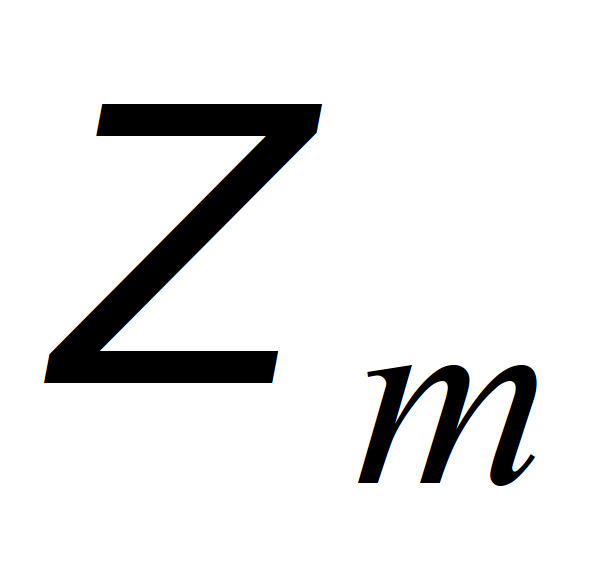
\includegraphics[width=0.3228in,height=0.3098in]{crypt-img/crypt-img55.png} .

Відкритий текст 
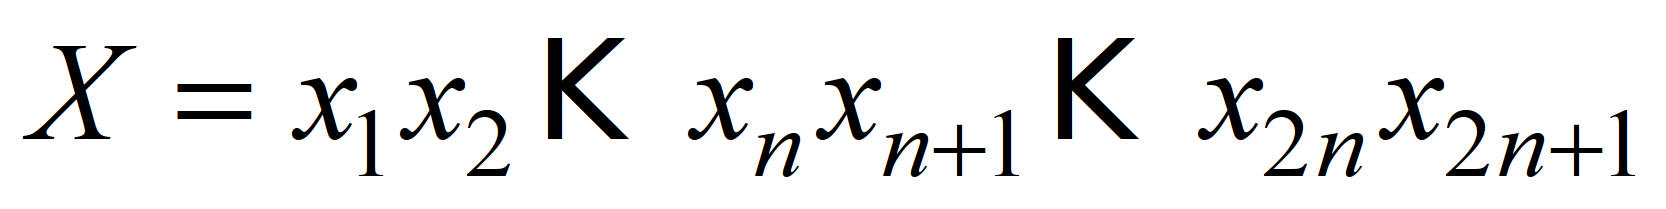
\includegraphics[width=2.5638in,height=0.3228in]{crypt-img/crypt-img56.png} …
розбивається на блоки по \textit{n }символів, кожний з блоків шифрується
секретним ключем, який задається підстановкою:

$$

де  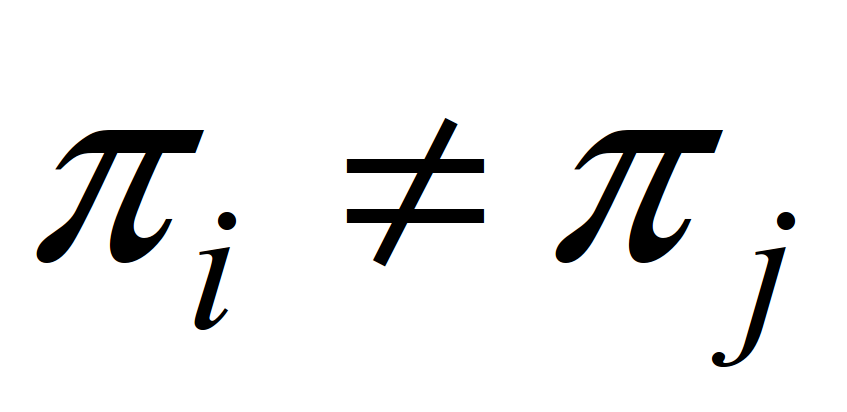
\includegraphics[width=0.6811in,height=0.3339in]{crypt-img/crypt-img58.png} 
при  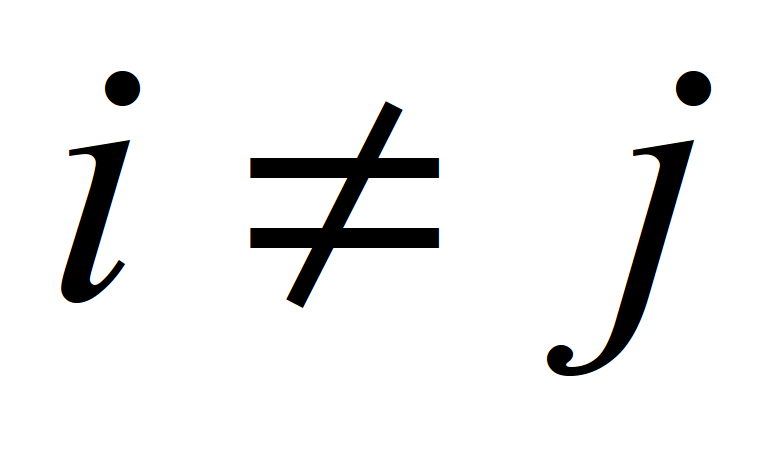
\includegraphics[width=0.4402in,height=0.252in]{crypt-img/crypt-img59.png}
,  $\pi _i}\in \left\{\;1,2,\dots,n\;\right\$. Букви в
кожному блоці переставляються згідно цієї підстановки за правилом 
$y_i}=x_{k^{{-1}(imod}n)+\left(\lceil i/n\rceil -1\right)\;\;n$,
 де   $\lceil t\rceil $ - верхня ціла частина дійсного числа
$t$\textit{,  } $i$mod\textit{n }
$?\left\{\;1,2,\dots,n\left.\right\}\right.$, зокрема 
$mn$mod$n$\textit{=$n$\textit{, } $y_i$  {}- це 
$i$\textit{{}-}а  буква шифрованого тексту $Y$=
$y_1y_2\dotsy_ny_{n+1}\dotsy_{2n}y_{2n+1}.}\text{.\text{.$
Відкритий текст законним користувачем отримується з шифрованого аналогічним
чином за допомогою підстановки $k$:  
$x_i}=y_{k(imodn)+\left(\lceil i/n\rceil -1\right)\;\;n$, 
$i$=1,2,3,...

\textit{Приклад}. 

Нехай  
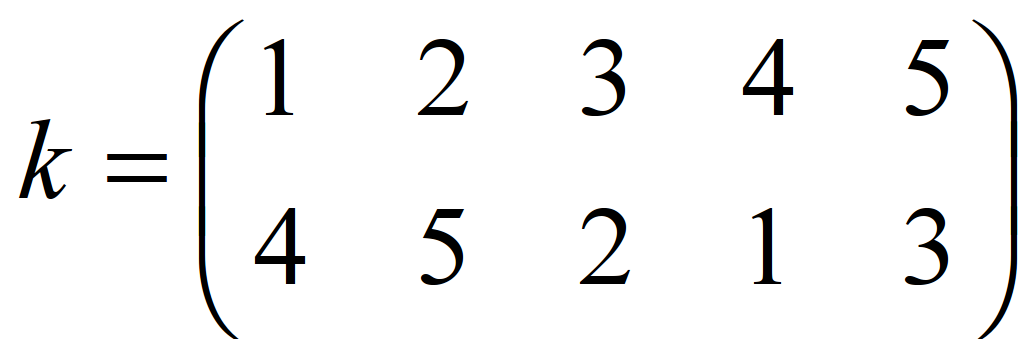
\includegraphics[width=1.8071in,height=0.598in]{crypt-img/crypt-img60.png} , 
тоді  
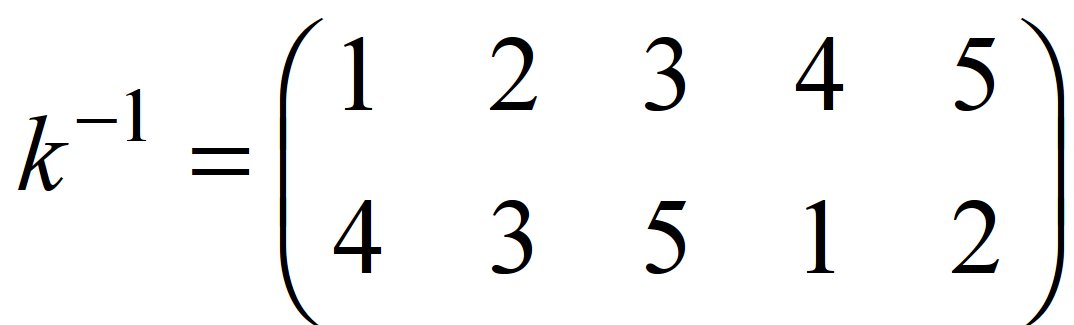
\includegraphics[width=1.9835in,height=0.5992in]{crypt-img/crypt-img61.png} .

Відкритий текст: \textit{шифрування}. Зашифрований текст: \textit{рфушиннява}. 

\textit{Потужність ключового простору загального шифру перестановки} (включаючи
тотожний ключ) з розміром блоку $n$дорівнює  $|K|=n$!  Ця
величина дуже швидко (експоненційно)  зростає з ростом величини блока. Так для 
$n$= 10, 20, 30  потужність буде відповідно 3,6
$?10}^{6}$,  2,4 $?\text{10}^{\text{18$,   $2,7\times
10}^{\text{32}$.

 Проте, при ,,ручному'' шифруванні  вибирати,  зберігати,
запам'ятовувати довільні  секретні  ключі з множини великої
потужності було украй незручно.  Тому на практиці використовувалися більш
прості, але зручніші шифри перестановки.


\bigskip


\bigskip

\section{Історичні шифри перестановки}


\bigskip


\bigskip

1) \textit{Шифр Скитала} (запис ВТ на стрічці, що намотана на барабан (скитал),
ключ --- діаметр барабану, див. лекцію 1);

\liststyleWWviiiNumxli
\begin{enumerate}
\item \textit{Шифр частоколу} висоти $h$\textit{(}\textit{h
}\textit{{}- }секретнийключ\textit{)}. Приклади:
\end{enumerate}
Відкритий текст: \textit{частокол}. 

ВТ записується в «частокoл», ШТ зчитується по рядках:

$$h$\textit{=}2
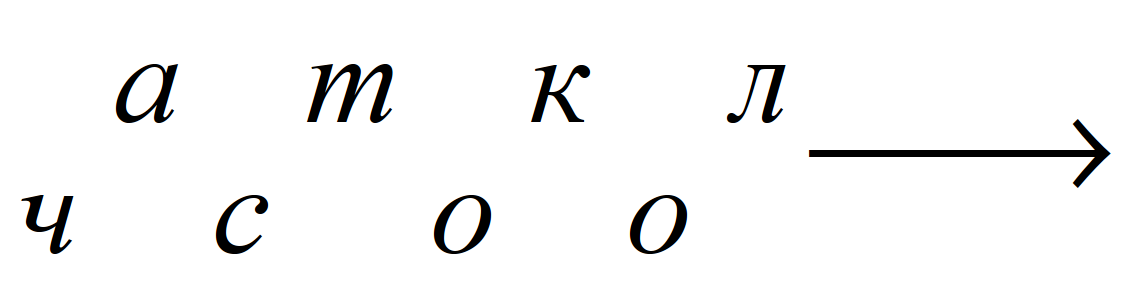
\includegraphics[width=1.7598in,height=0.4681in]{crypt-img/crypt-img62.png} 
шифрований текст: \textit{атклчсоо}.
\par}

$$h$\textit{=}3 
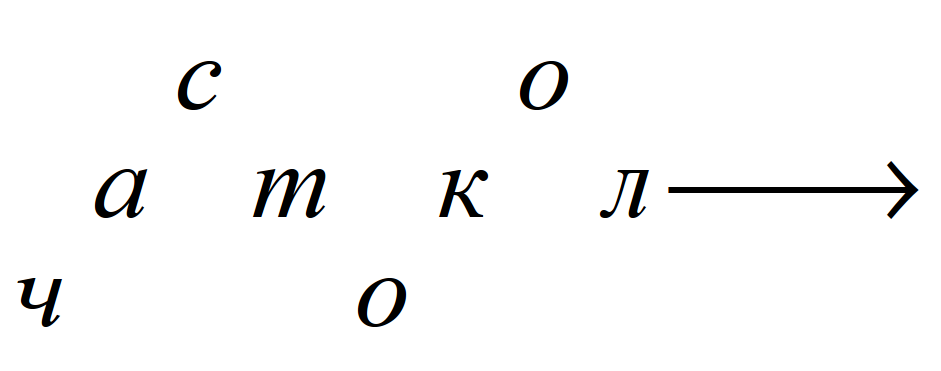
\includegraphics[width=1.7193in,height=0.6799in]{crypt-img/crypt-img63.png} 
шифрований текст: \textit{соатклчо}.
\par}

\liststyleWWviiiNumxli
\setcounter{saveenum}{\value{enumi}}
\begin{enumerate}
\setcounter{enumi}{\value{saveenum}}
\item \textit{Шифри обходу} (маршрутні шифри): блок відкритого тексту
записується за певним маршрутом (обходом) в яку-небудь геометричну фігуру, в її
вузли, або у вершини графа, або в клітини таблиці тощо заносяться букви, блок
шифрованого тексту виходить шляхом зчитування літер іншим маршрутом (обходом)
вузлів, вершин, клітинок. Геометрична фігура, шляхи запису ВТ і зчитування ШТ є
секретними ключами.
\end{enumerate}
 Розглянемо найвідоміші шифри обходу.

\liststyleWWviiiNumxli
\setcounter{saveenum}{\value{enumi}}
\begin{enumerate}
\setcounter{enumi}{\value{saveenum}}
\item  \textit{Таблична перестановка}. 
\end{enumerate}
\textit{Проста таблична перестановка}: відкритий текст записується по рядках,  а
шифрований - прочитується по стовпцях таблиці. \textit{Ускладнена таблична
перестановка}: обхід таблиці як при записі відкритого тексту, так і при
списуванні шифрованого  може бути ускладнений (див. рис. 7.1).

  

\begin{figure}
\centering
\begin{minipage}{5.8634in}
{\centering\bfseries
 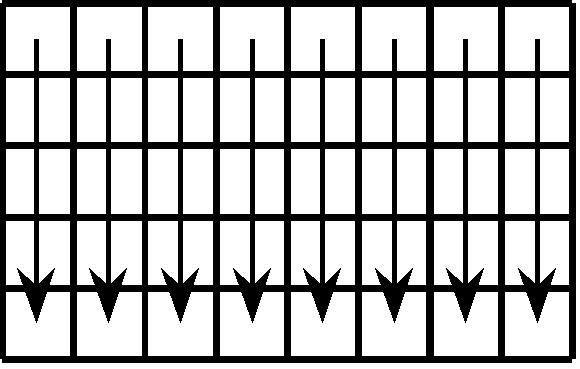
\includegraphics[width=1.6201in,height=1.0209in]{crypt-img/crypt-img64.png}
\ \  
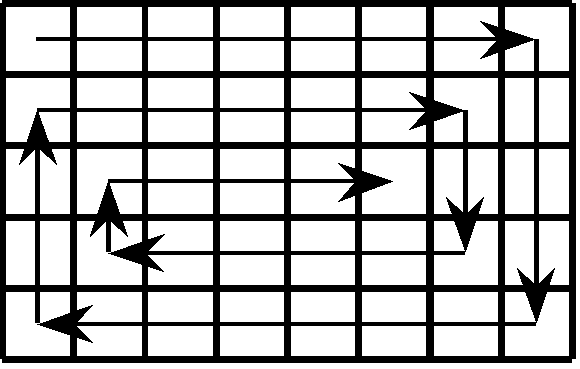
\includegraphics[width=1.6201in,height=1.0102in]{crypt-img/crypt-img65.png} 
\ \ 
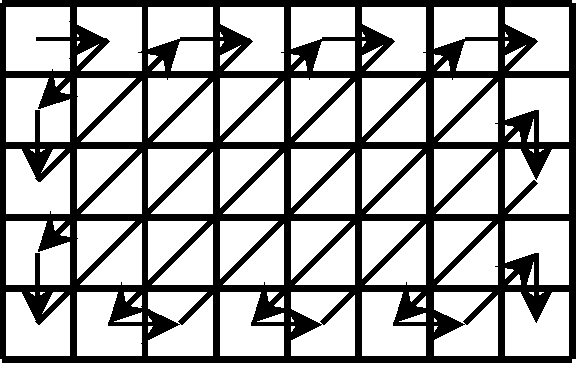
\includegraphics[width=1.6201in,height=1.0209in]{crypt-img/crypt-img66.png} 
\par}
\end{minipage}
\end{figure}
\begin{figure}
\centering
\begin{minipage}{5.4543in}
$$


\bigskip
\end{minipage}
\end{figure}

\bigskip


\bigskip

Можливе також використання додаткового ключа: деякі клітинки пропускаються при
запису (див. рис. 7.2). Тоді потужність ключового простору при відомих
маршрутах та розмірі таблиці складає 
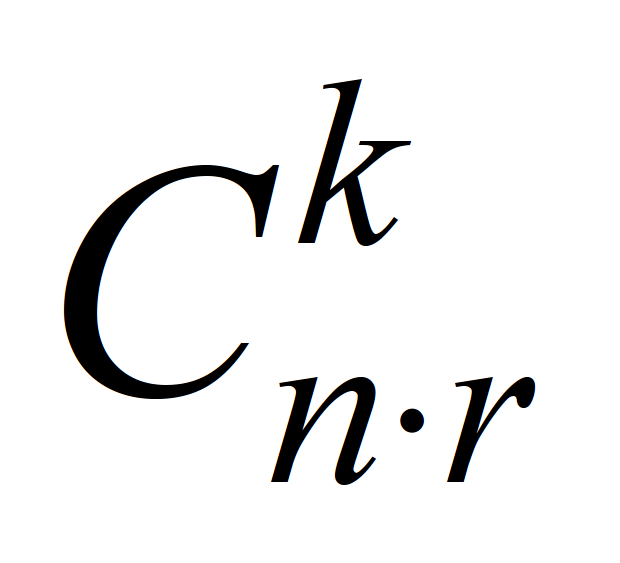
\includegraphics[width=0.4016in,height=0.3681in]{crypt-img/crypt-img67.png} ,
де $n$, \textit{r }--- розміри таблиці, а $k$--- кількість
невживаних клітинок, тобто тих, в які не записуються букви тексту. Треба
сказати, що невдалий  вибір маршрутів та порожніх клітинок суттєво впливає на
надійність шифру. Інші ускладнення шифрів перестановки --- використання не
прямокутної таблиці, а, наприклад, у вигляді ромбу, більш складної фігури.


\bigskip


\bigskip

{\centering 
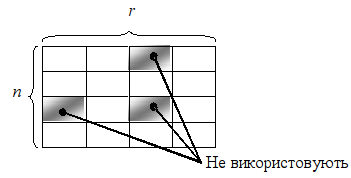
\includegraphics[width=2.8854in,height=1.3854in]{crypt-img/crypt-img68.png}
\par}



\begin{figure}
\centering
\begin{minipage}{6.1283in}
$$\textbf{Рис. 7.2. }\textit{Таблична перестановка з використанням порожніх
}\textit{\textcolor[rgb]{0.0,0.5019608,0.0}{клітинок}}
\par}


\bigskip


\bigskip


\bigskip


\bigskip
\end{minipage}
\end{figure}
Широке поширення набули шифри з вертикальною 


\bigskip

\textbf{ }Широке \textcolor[rgb]{0.0,0.5019608,0.0}{поширення} набули
\textit{шифри з вертикальною і горизонтальною перестановкою}: блок ВТ
записується  в прямокутну таблицю відповідного розміру по рядках в деякому
заданому порядку рядків, а прочитується по стовпцях відповідно до заданого
порядку стовпців. Розмір таблиці, а також порядки рядків і стовпців є
секретними ключами. Для кращого запам'ятовування в якості
секретних ключів бралися  два слова з різними буквами кожне, число букв в яких
рівне числу рядків і стовпців відповідно. Порядок рядків і стовпців визначався
порядком слідування букв ключового слова в алфавіті.  При відомому розмірі
таблиці  $n$ $?$ \textit{r }\textit{ потужність ключового простору
}буде $n!\times r!$.

\liststyleWWviiiNumxli
\setcounter{saveenum}{\value{enumi}}
\begin{enumerate}
\setcounter{enumi}{\value{saveenum}}
\item \textit{Шифри перестановки за допомогою маршрутів Гамільтона} в графі
(див. рис. 7.3). Граф і маршрути є секретними ключами.
\end{enumerate}

\bigskip

{\centering\bfseries
[Warning: Draw object ignored]
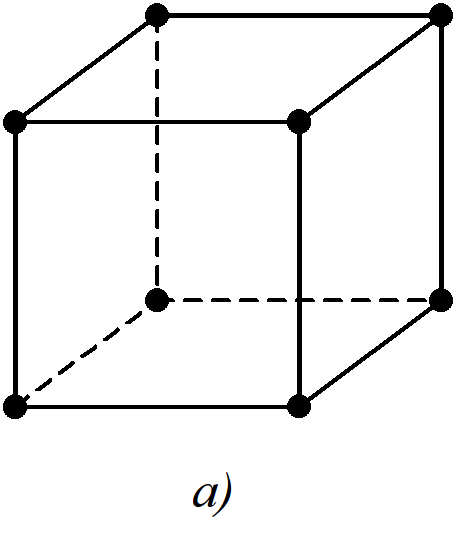
\includegraphics[width=1.2811in,height=1.5209in]{crypt-img/crypt-img69.png}
\ \ \ \ 
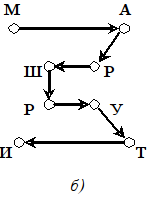
\includegraphics[width=1.2189in,height=1.7335in]{crypt-img/crypt-img70.png} 
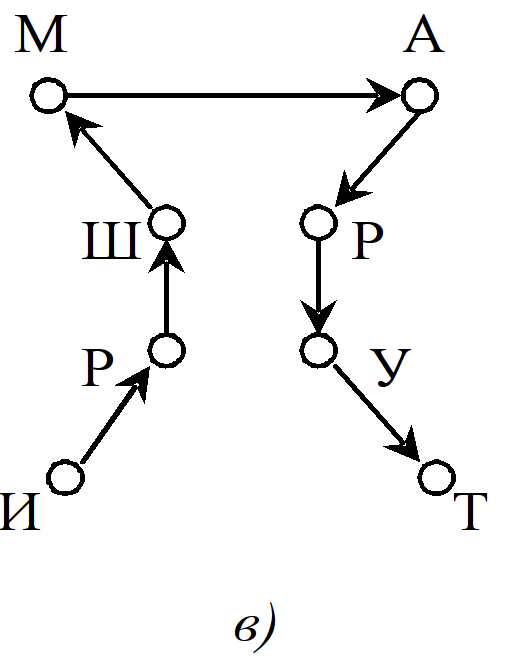
\includegraphics[width=1.2189in,height=1.6665in]{crypt-img/crypt-img71.png} 
\par}


\bigskip

$$\textbf{Рис. 7.3. }\textit{Приклад реалізації шифру, побудованого на
Гамільтонових маршрутах}
\par}

$$а) --- \textit{заданий граф(куб)}, б) --- \textit{обхід при записі відкритого
тексту}, 
\par}

$$

$$


\bigskip

\liststyleWWviiiNumxli
\setcounter{saveenum}{\value{enumi}}
\begin{enumerate}
\setcounter{enumi}{\value{saveenum}}
\item \textit{Грати Кардано} --- це шифр перестановки, секретним ключем якого є
сітка (таблиця) розміром  $2n\times 2n$,  в якій вирізується  $n^{2$
віконець (клітинок). У віконця грат записується четверта частина блоку
відкритого тексту і грати повертається на 
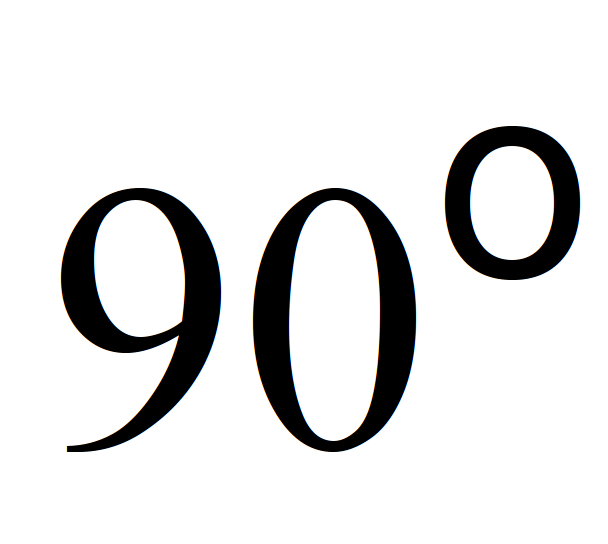
\includegraphics[width=0.3063in,height=0.2819in]{crypt-img/crypt-img72.png} ,
знов у віконця, які всі виявляться вільними, записується продовження  ВТ, грати
знову повертаються на 
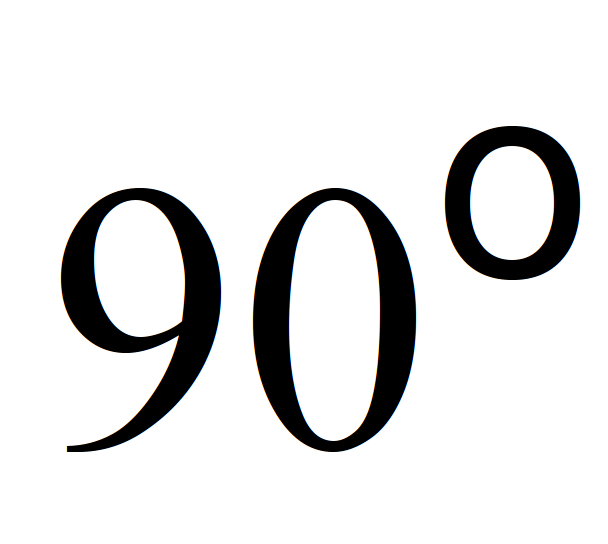
\includegraphics[width=0.3063in,height=0.2819in]{crypt-img/crypt-img73.png}  і
всі віконця  знову будуть порожніми. Після запису продовження ВТ грати
повертаються останній 4 раз на 
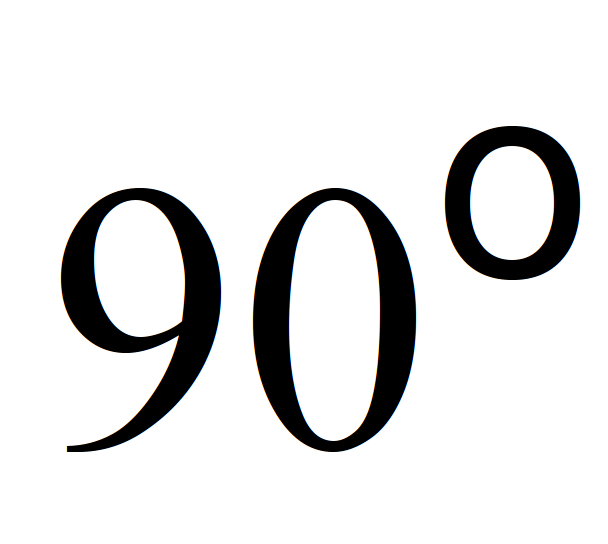
\includegraphics[width=0.3063in,height=0.2819in]{crypt-img/crypt-img74.png}  і
в клітини, що звільнилися, записується частина ВТ, що залишилася. 
\end{enumerate}
Порожні клітини в кінці, якщо текст коротший за розмір блоку (грати),
доповнюються, наприклад, буквами з алфавіту. Вирізані грати --- секретний ключ.
Як вибрати довільний секретний ключ, тобто вирізати віконця з необхідними
властивостями, демонструє рис. 7.4. Нумерація в клітинках --- для правильного
вибору ключа. Вибирається довільним чином  $n^{2$ різних чисел для
вирізування віконець під ключ. \textit{Потужність} \textit{ключового простору}:

\begin{figure}
\centering
\begin{minipage}{}
 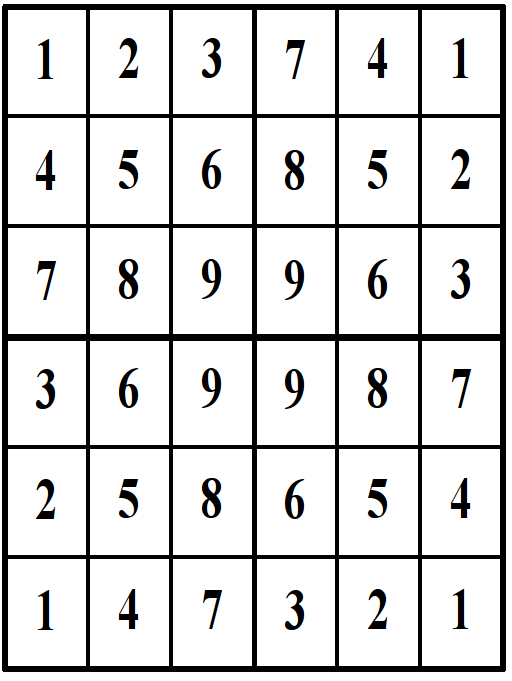
\includegraphics[width=1.9374in,height=1.9374in]{crypt-img/crypt-img75.png} 
\end{minipage}
\end{figure}
\begin{figure}
\centering
\begin{minipage}{2.3575in}
$$
\end{minipage}
\end{figure}
$$

Модифікація --- перестановка запису в клітинах, тоді  
$|K|=2^{2n^{{2}}}((n^{2}{)!)}$,  і вже при  $n=4$   $|K|\approx
10}^{\text{23}$.

\liststyleWWviiiNumxli
\setcounter{saveenum}{\value{enumi}}
\begin{enumerate}
\setcounter{enumi}{\value{saveenum}}
\item \textit{Магічні квадрати} --- матриці розміром  $n\times n$, в яких
розташовані числа від 1 до  $n^{2$ таким чином, що сума чисел в кожному
рядку, у кожному стовпці та у двох головних діагоналях однакова. Наприклад: 
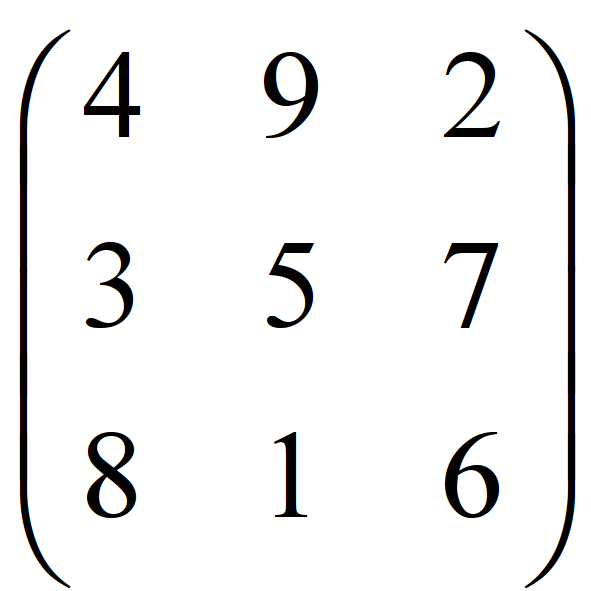
\includegraphics[width=0.778in,height=0.778in]{crypt-img/crypt-img76.png} .
Відкритий текст записується по рядках, а прочитується у порядку, що
визначається числами. При $n$=3 наведений магічний квадрат єдиний з
точністю до повороту, для $n$=4  їх  880, для $n$=5 --- їх вже
близько 250 тисяч і далі число магічних квадратів швидко зростає. Побудова
магічних квадратів і підрахунок їх числа - складна математична задача. 
\item Ще одна з модифікацій шифру перестановки --- \textit{шифри подвійної
(потрійної) перестановки}, що задаються, наприклад,  двома (трьома) різними
таблицями.
\end{enumerate}
 Описані шифри перестановки за сучасними поняттями  не є стійкими, особливо при
нападі на основі відкритого тексту і вибраного тексту.


\bigskip

\section{Загальна класифікація основних класичних  шифрів}


\bigskip

Шифри заміни (підстановки)

Моноалфавітна заміна:

Цезаря;

афінна;

загальна моноалфавітна;

Поліалфавітна заміна:

біграмна;

шифри Хілла (шифри $l$-грамної афінної заміни);

шифр Віженера;

шифр з автоключем;

шифр з рядка, що біжить;

шифр Вернама;

Шифри перестановки (див. вище)

Шифри гаммування:

модульне гаммування;

табличне гаммування;


\bigskip

Аналітичні шифри.

Кодування:

символьне;

змістовне;

Комбіновані (композиційні).

Відзначимо,  що класичні  шифри, взагалі кажучи, не є стійкими при сучасних
методах і техніці криптоаналізу з використанням ЕОМ.


\bigskip

\section{Принципи Шеннона побудови стійких  шифрів}


\bigskip


\bigskip

$\blacklozenge$ \textit{Розсіювання} (\textit{розповсюдження помилок}) --- це
властивість криптографічного перетворення, при якому зміна одного будь-якого 
символу (біту) на вході спричиняє за собою зміну певної (великої)  кількості
символів (бітів) на виході. Це принцип розповсюдження впливу кожного знаку 
відкритого тексту або ключа на багато знаків шифртексту. Однією з формалізацій
цієї властивості  в сучасних теоріях є так званий лавинний ефект.

$\blacklozenge$ \textit{Перемішування }--- це властивість криптографічного
перетворення, яка суттєво ускладнює взаємозв'язок статистичних
 і аналітичних характеристик елементів зашифрованого тексту порівняно з
подібними взаємозв'язками відкритого тексту . 

 Шеннон запропонував будувати стійкі шифри відповідно до цих принципів за
допомогою чергування різних криптографічних перетворень, кожне з яких саме по
собі не стійке, наприклад, за допомогою класичних перетворень підстановки,
перестановки, гамування тощо.


\bigskip


\bigskip

\section{Контрольні питання}


\bigskip


\bigskip

\liststyleWWviiiNumxvii
\begin{enumerate}
\item Чим відрізняються шифри заміни (підстановки) від шифру перестановки?
\item Чому дорівнює потужність ключового простору в загальному шифрі
перестановки з розміром блоку $n$?
\item Скільки ключів має шифр табличної перестановки з перестановкою рядків і
стовпчиків? 
\item Які ви знаєте шифри обходу? Що є таємним ключем у таких шифрах?
\item Поясніть правило шифрування в так званих гратах Кардано. Яким чином
вибирається таємний ключ?
\item Дайте означення магічного квадрату.
\item Що таке комбіновані шифри?
\item Сформулюйте принципи Шеннона розсіювання  та перемішування. 
\end{enumerate}

\bigskip


\bigskip


\bigskip


\bigskip


\bigskip

{\bfseries
ЛЕКЦІЯ  8}


\bigskip

{\centering\bfseries
РОТОРНІ  ШИФРАТОРИ
\par}


\bigskip


\bigskip

Роторні шифратори  ---  це механічні або електромеханічні пристрої, в яких
основною деталлю є ротори  ---  диски, що обертаються, ---  звідси і назва. Роторні
шифратори були дуже широко поширені під час Другої світової війни. Німецька
Enigma --- головна шифрувальна машина Вермахту --- була роторним шифратором. Були
шифратори такого типу у всіх арміях, що воювали. Застосовувалися вони і після
війни, деякі --- аж до 70-х років минулого століття.

Всі роторні шифратори реалізують шифр Віженера з дуже великим періодом.
Щоправда, існує одна, не дуже істотна, відмінність: у шифрі Віженера ВТ
посимвольно складається з ключовою послідовністю, в роторному шифраторі ---
віднімається:


\bigskip

$$\begin{matrix}{c_i}=k_i}-p_i}}\hfill\null
\\p_i}=k_i}-c_i}\hfill\null \end{matrix}\hfill $$


\bigskip

де  $p_i}-$  $i$-та буква ВТ,   $c_i}-i$-та буква ШТ, 
$k_i}-i$-та буква ключа. Таким чином, шифрування і розшифрування
здійснюються за допомогою тієї ж самої процедури: одна й та ж машина шифрує й
розшифровує. Так як періоди шифрів Віженера, що реалізуються роторними
шифраторами, величезні, то метод криптоаналізу шифру Віженера, вивчений нами
раніше, до них безпосередньо не придатний.

Роторні шифратори можна підрозділити на колесні (чисто механічні) і власне
роторні --- електромеханічні пристрої.

Розглянемо будову і криптоаналіз колесного шифратора на прикладі машини Хагеліна
(застосовувалася під час війни в американській армії під назвою М-209). Головна
його деталь --- диск (колесо), по ободу якого нанесені букви. Таких дисків 6.
Диски пов’язані з системою зубчатих коліс. Кожному диску відповідає зубчате
колесо, кількість зубців на якому така сама, як і кількість букв на диску. 

Зубчаті колеса насаджені на загальну вісь. Кількість зубців у них різна: 26, 25,
23, 21, 19 і 17 відповідно. Так само на першому диску нанесені всі букви
латинського алфавіту, на другому --- всі, окрім останньої, на третьому --- перші 23
букви алфавіту і т.д., на шостому --- перші 17 букв. На кожному такті роботи
зубчаті колеса повертаються на один зубець, відповідно і диски --- на одну букву.
Так влаштовано, що після кожного повороту  (на кожному такті)  букви у
визначеному  місці  шикуються  в рядок. Якщо на першому  такті роботи рядок має
вигляд АА…А, то далі так:

\begin{figure}
\centering
\begin{minipage}{0.0161in}

\bigskip
\end{minipage}
\end{figure}
$$

$$

$$

 17-й такт  \textbf{Q Q Q Q Q Q}

 18-й такт  \textbf{R R R R R А}


\bigskip

За 17 тактів останнє колесо зробило повний оберт. Оскільки числа зубців взаємно
прості, то період послідовності 6-буквених рядків дорівнює 


\bigskip

\begin{equation*}
{26}\times \text{25}\times \text{23}\times \text{21}\times \text{19\times
17}\approx \text{101}\;млн}\text{.
\end{equation*}

\bigskip

Це більше кількості букв у будь-якій енциклопедії. Проте самі ці букви
використовуються лише для встановлення на початку роботи всіх коліс шифратора у
певну позицію: наприклад, коли рядок у віконці складається з усіх букв А . Річ
у тому, що біля кожної букви на кожному диску є штифт, який може бути висунутий
(1) або втиснений (0). Тоді кожному рядку букв відповідає 6-бітовий рядок.
Всього 6-бітових рядків  2\textsuperscript{6}= 64, тому вони на періоді багато
разів повторюватимуться, але в різному порядку. Період послідовності 6-бітових
рядків такий самий (\~{} 101 млн.). Над дисками розташована клітка --- циліндр із
спиць. На кожній спиці --- по два повзунки, які можна встановлювати навпроти
будь-якого колеса або в нейтральну позицію. Збоку є друкуюче колесо, по ободу
якого нанесений весь алфавіт. Є також покажчик, на якому виставляється буква
ВТ, що підлягає шифруванню. У кожен момент одна буква на друкуючому колесі
знаходиться у робочій позиції (віддруковується на паперовій стрічці).
Шифрування відбувається таким чином: коли на покажчику виставляють букву ВТ,
вона стає в робочу позицію на друкуючому колесі. Але одночасно повертаються всі
диски на один зубець і клітка робить повний оберт. При обертанні  клітки
висунуті штифти і повзуни, що стоять навпроти них, взаємодіють через систему
важелів, при цьому  вискакують спиці і повертають друкуюче колесо на число
позицій, відповідне букві ключової послідовності. А додати або відняти букву
ключа --- це якраз і означає повернути друкуюче колесо на відповідне число
позицій в ту або іншу сторону. Ключем є розташування штифтів на всіх колесах і
повзунів на спицях.


\bigskip


\bigskip


\bigskip

 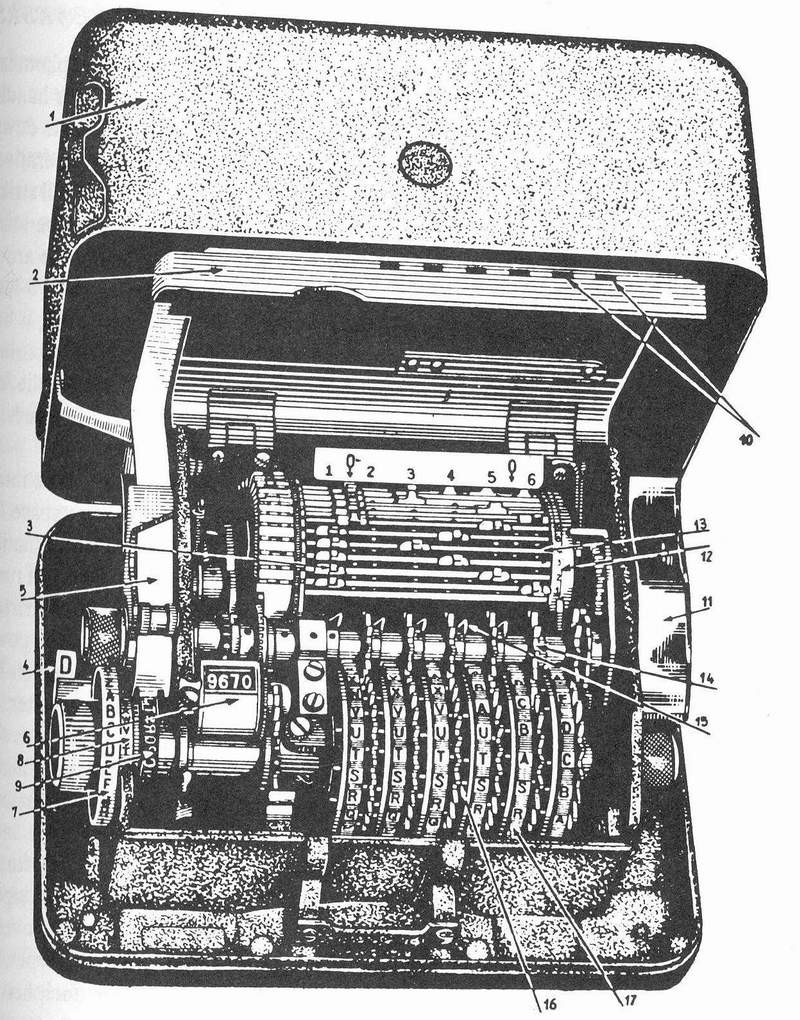
\includegraphics[width=5.6252in,height=6.5555in]{crypt-img/crypt-img77.jpg}
[Warning: Draw object ignored][Warning: Draw object ignored]Математично процес
шифрування можна зобразити таким чином: нехай є таблиця з 64 комірок
(наприклад, квадратна 8 $?$ 8). Її комірки занумеруємо числами від 0 до 63
(тобто 6-бітними векторами). У таблиці якимось чином записані букви алфавіту,
по одній у комірці --- певно, деякі з них повторюються.  Заповнення таблиці
відповідає розташуванню повзунів на спицях клітки. Значення 6-бітового рядка 
(з висунутих і втиснутих штифтів, що стикаються з повзунами) на i-му такті
визначає номер комірки в таблиці . Буква, записана в цій комірці, якраз і буде 
$i-$ ю буквою ключової послідовності. 

\begin{figure}
\centering
\begin{minipage}{5.8043in}
$$


\bigskip

{\centering\itshape
1--- футляр, 2 --- зубчате колесо, 3 --- важіль, 4 --- диск з алфавітом,  5 --- висунутий
штифт, 6 ---  спиця, 7 --- повзун у нейтральній позиції, 8 --- паперова стрічка, 9 ---
покажчик букви, що шифрується, 10 --- покажчик кількості зашифрованих знаків, 11
---  колесо, що друкує
\par}


\bigskip
\end{minipage}
\end{figure}
\begin{figure}
\centering
\begin{minipage}{0.4043in}
11
\end{minipage}
\end{figure}
\begin{figure}
\centering
\begin{minipage}{0.4126in}
 7


\bigskip

 8


\bigskip


\bigskip

 9


\bigskip

 10


\bigskip


\bigskip
\end{minipage}
\end{figure}
\begin{figure}
\centering
\begin{minipage}{0.2835in}
3  1
\end{minipage}
\end{figure}
\begin{figure}
\centering
\begin{minipage}{0.2209in}
6
\end{minipage}
\end{figure}
\begin{figure}
\centering
\begin{minipage}{0.3335in}
1  1
\end{minipage}
\end{figure}
\begin{figure}
\centering
\begin{minipage}{0.1252in}
2
\end{minipage}
\end{figure}
\begin{figure}
\centering
\begin{minipage}{1in}
 5
\end{minipage}
\end{figure}
\begin{figure}
\centering
\begin{minipage}{0.1252in}
4
\end{minipage}
\end{figure}
\begin{figure}
\centering
\begin{minipage}{0.2209in}

\bigskip
\end{minipage}
\end{figure}
\begin{figure}
\centering
\begin{minipage}{0.3252in}

\bigskip
\end{minipage}
\end{figure}
\begin{figure}
\centering
\begin{minipage}{0.1957in}

\bigskip
\end{minipage}
\end{figure}
\begin{figure}
\centering
\begin{minipage}{0.4374in}

\bigskip
\end{minipage}
\end{figure}
\ \ Отже, ключ складається з 2-х частин: заповнення таблиці (тобто розташування
повзунів) і положення всіх штифтів на дисках. Можливість визначення ключа
частотним аналізом грунтується на тому, що букви ключової послідовності
нерівноймовірні. Дійсно, оскільки комірок 64, а букв в алфавіті (латинському)
26, то в кращому разі 12 букв зустрінуться в таблиці тричі (матимуть
імовірність 3/64), а 14 букв --- двічі (їх імовірність 2/64). Складаючи
нерівноймовірну ключову послідовність з нерівноймовірним ВТ, одержуємо
нерівноймовірні букви ШТ. Як це використати при криптоаналізі? Запишемо ШТ у
вигляді таблиці з рядками довжини 17:

$$y$\textsubscript{1},  $y$\textit{\textsubscript{2}}, … ,\textit{ 
y}\textit{\textsubscript{17}}
\par}

$$y$\textit{\textsubscript{18}},  \textsubscript{
$y$\textit{\textsubscript{19}}, …,
$$

$$

Кожен стовпець таблиці зашифрований при одному і тому ж положенні останнього
колеса, тобто при певному значенні останнього біта в 6-бітовому рядку --- 0 або
1. Розділимо таблицю з 64 кліток на дві частини: ті комірки, яким відповідає
номер з нулем на останньому місці, і ті комірки, номери яких закінчуються на 1,
тобто з парними та непарними номерами. Якщо вибирати букви випадково з якоїсь
частини таблиці (першої або другої), то розподіли букв для 1-ї та 2-ї частини
таблиці будуть різні. Отже, частоти букв у стовпцях ШТ в нашій таблиці
належатимуть одному з двох типів розподілу (що відповідають 0 або1 на даному
місці 6-го колеса). Методи математичної статистики дозволяють розділити ці два
розподіли. Отже, деяким стовпцям ШТ ми можемо приписати значення 0, а іншим --- 1
і таким чином визначити положення штифтів на 6-му колесі (можна 0 і 1 поміняти
місцями --- це неістотно). Так само, виписуючи ШТ в таблицю з рядками довжини 19,
відновлюємо положення штифтів на 5-му колесі і т.д.

Коли всі штифти розставлені, можна змоделювати роботу роторів і одержати
послідовність 6-бітових рядків --- ту, яка і з'являлася при
шифруванні. Запишемо поряд з нею послідовність букв ШТ. Кожна буква ШТ
зашифрована при відповідному значенні 6-бітового рядка. Випишемо 64 стовпці: у
стовпець з номером 000…0 випишемо букви ШТ, зашифровані при нульовому
6-бітовому рядку, в стовпець з номером 000…1 випишемо букви ШТ, зашифровані,
коли серед штифтів, що стикалися з повзунами, був висунутий лише останній, і
т.д. У кожному стовпці букви зашифровані шифром Цезаря із зсувом, що відповідає
букві, яка стоїть в таблиці  в комірці з номером, рівним номеру стовпця. Тобто
частоти букв в стовпці такі ж, як у мові, але зсунуті на номер букви алфавіту,
що стоїть у відповідній комірці. Таким чином визначаємо заповнення таблиці ---
другу частину ключа.

При знаходженні ключа можливі помилки. Їх можна виправити. Розшифруємо текст за
допомогою знайденого ключа. На деяких місцях в дешифрованому тексті будуть
помилки. Якщо, наприклад, помилки зустрічаються на місцях з номерами виду 
17\textit{к+}2, це означає, що другий штифт на останньому колесі встановлений
невірно, змінюємо його на протилежний і т.д.

Для визначення ключа в машині Хагеліна достатньо близько 2000 знаків (методом
дещо хитрішим, ніж описаний), а при відомому ВТ --- близько 500. (Складаємо ВТ з
ШТ, одержуємо ключову послідовність. Аналізуємо її так само. Тепер в стовпці з
номером, наприклад, 000…0 повинна стояти одна й та сама буква. Якщо десь
з’явилась інша --- значить помилка в установці штифта.)

Машина Хагеліна --- чисто механічний пристрій, тому застосовувалася в польових
умовах. У штабах використовувались електромеханічні роторні шифратори (до їх
числа належить і Enigma). У них теж основна частина --- ротори, по ободу яких
нанесений алфавіт. Біля кожної букви на лівій і правій стороні ротора контакти.
Ліві, наприклад, вважатимемо вхідними, а праві --- вихідними. Вхідний контакт
кожної букви сполучений усередині ротора провідником з вихідним контактом
деякої іншої букви. Якщо, наприклад, вхідний контакт букви В сполучений з
вихідним контактом букви М, то при подачі струму на вхідну букву В (буква ВТ)
на виході одержимо струм на контакті букви М (буква ШТ). Таким чином, ротор
здійснює деяку підстановку на алфавіті.

{\centering 
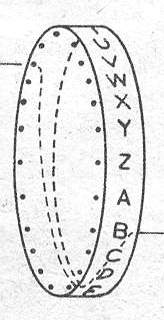
\includegraphics[width=1.7083in,height=3.3335in]{crypt-img/crypt-img78.jpg}
\par}

\begin{figure}
\centering
\begin{minipage}{0.9374in}
Буква ШТ
\end{minipage}
\end{figure}
\begin{figure}
\centering
\begin{minipage}{0.9665in}
Буква ВТ
\end{minipage}
\end{figure}
$$


\bigskip

Роторів декілька (3 --- 5), насаджені на загальну вісь. У всіх однакове число
контактів (26 або більше, наприклад, 128 --- код ASCII). Ротори можуть обертатися
один відносно одного. Після повороту контакти сусідніх роторів
з'єднуються. Результуюче перетворення залежить на кожному
кроці від підстановок, реалізованих перемичками усередині кожного ротора і від
положення роторів один щодо одного. Можна вибрати різні закони руху роторів. У
Enigma --- за принципом лічильника: коли останнє колесо робить повний оберт,
передостаннє зміщується на одну букву і т.д.



\begin{figure}
\centering
\begin{minipage}{1in}
Контакти
\end{minipage}
\end{figure}

\bigskip

{\centering 
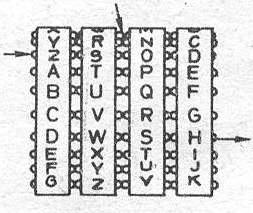
\includegraphics[width=2.6354in,height=2.2189in]{crypt-img/crypt-img79.jpg}
\par}

\begin{figure}
\centering
\begin{minipage}{0.6583in}
Вихід
\end{minipage}
\end{figure}
\begin{figure}
\centering
\begin{minipage}{0.5417in}
Вхід
\end{minipage}
\end{figure}
$$


\bigskip

\ \ Криптоаналіз роторних шифраторів досить складний. Полегшується за наявності
комплекту роторів. Тоді задача полягає в знаходженні короткочасного ключа ---
початкового положення роторів, роторів, вибраних з комплекту, і деяких
перестановок, що виконувалися над ВТ і ШТ до і після шифрування. У Enigma
спочатку було просто 3 ротори, потім --- комплект з 5-ти роторів, з яких 3
кожного разу вибиралися і ставилися в машину. (Під час війни англійці здобули
комплекти роторів і тому змогли розколоти Enigma).

Довгостроковий ключ --- перемички усередині роторів (підстановки, здійснювані
кожним ротором).

\ \ Методи знаходження довгострокового ключа були запропоновані лише в  70-х
роках. Розглянемо ідею такого криптоаналізу роторного шифратора при відомому
ВТ. Нехай ротори рухаються за принципом лічильника. Для простоти вважатимемо,
що в початковий момент всі ротори знаходяться в початковому положенні (нульовий
зсув один щодо одного). Вхідні контакти першого ротора на кожному такті
стикаються з нерухомими контактами, кожен з яких відповідає певній букві
алфавіту; саме на них і подається чергова буква ВТ для шифрування.

\ \ Мета криптоаналізу --- знайти підстановки, здійснювані роторами.

\ \ Нехай $m$ --- число букв алфавіту, \textgreek{p --- }підстановка,
здійснювана першим ротором.

\ \ Неважко бачити, що буква на вході другого ротора у момент $t$
дорівнює
\textit{\textgreek{p}}($x$\textit{\textsubscript{t}}\textit{+$t$)
-$t$, де   $x_t$ --- $t$\textit{{}-}абуква ВТ,
1$\leq$$t$\textit{\textless$m$. Дійсно, оскільки ротор за
$t$тактів зсунувся на $t$позицій, то вхідний
сигнал, поданий на букву $x_t$, потрапить вже на букву 
$x_t$\textit{+t }на вході 1-го ротора. Далі в роторі сигнал по перемичці
проходить на букву \textit{\textgreek{p}}( $x_t$\textit{+$t$), що
на нерухомому вхідному контакті 2-го ротора відповідає букві
\textit{\textgreek{p}}( $x_t$\textit{+$t$) -$t$. 

При шифруванні відрізка тексту
$x$\textit{\textsubscript{km}}\textsubscript{+1},…,$x$\textit{\textsubscript{(}}\textit{\textsubscript{k}}\textit{\textsubscript{+1)}}\textit{\textsubscript{m}}
ротори з номерами  2, 3, … стоять, рухається лише перший ротор. Тому
перетворення, здійснюване всіма роторами, окрім першого, залежить лише від
номера відрізка  $k$. Позначимо його $S$\textit{\textsubscript{k}}.

Нехай на відрізку трапилася ситуація, коли, 
$x_{km}+i+i\neq
x_{km}+j+j,$ 
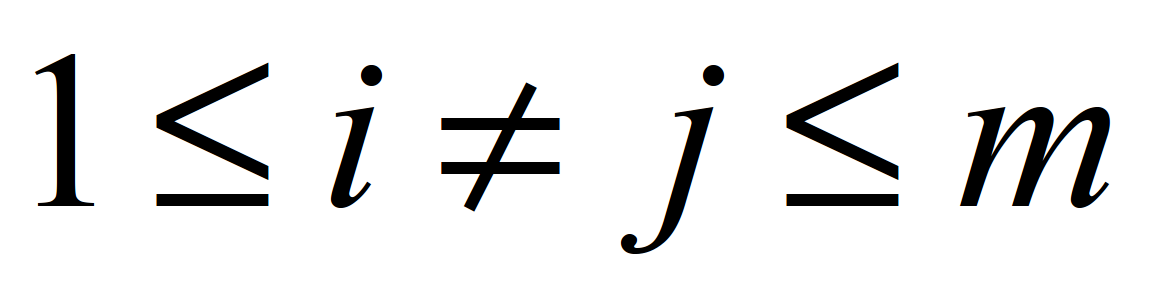
\includegraphics[width=0.861in,height=0.222in]{crypt-img/crypt-img80.png} , а 
$y_{km}+i}}=y_{\normalsubformula{km+j$,
тобто

$$S_k(\pi (x_{km}+i+i)-i)=S_k(\pi
(x_{km}+i+j)-j)$$

Але оскільки $S$\textit{\textsubscript{k}} --- взаємно{}-однозначна
відповідність, то

{\centering  $ $ $\pi (x_{km}+i+i)=\pi
(x_{km}+j+j)+i-j,$\par}

і ми одержуємо рівняння, що зв'язує значення  \textgreek{p }на
двох різних буквах. Маючи достатньо довгий текст, можемо набрати систему
лінійних рівнянь для визначення значень \textgreek{p }на всіх буквах. Знаючи
\textgreek{p }на першому роторі, можна так само визначити підстановку і для
другого, але він рухається у  $m$ разів повільніше --- потрібно набагато більше
матеріалу. Сучасні обчислювальні засоби дозволяють проводити криптоаналіз для
системи з декількох роторів, питання лише в наявності досить довгої пари
відрізків ВТ і ШТ . Для одного ротора можна знайти \textgreek{p, }маючи лише
ШТ.

Роторні шифратори були для свого часу вельми стійкими і довго використовувалися.
Зараз інформація передається і зберігається в електронному виді, так що
електромеханічні пристрої втратили своє значення, хоча принципи їх роботи
знаходять застосування і в сучасній криптографії.


\bigskip

\section{Контрольні питання}


\bigskip


\bigskip

\liststyleWWviiiNumxxxiv
\begin{enumerate}
\item Коли застосовувались роторні шифратори? Чому вони отримали таку назву?
\item Чим відрізняються колісні шифратори від власне роторних?
\item Опишіть основні риси будови машини Хагеліна. Який метод застосовується при
криптоаналізі шифру, що вона реалізує?
\item Який роторний шифратор використовувався німцями підчас Другої світової
війни? 
\item Що таке ротор? Яке перетворення на алфавіті він реалізує?
\item Чи піддаються роторні шифратори частотному криптоаналізу?
\end{enumerate}

\bigskip


\bigskip


\bigskip

{\bfseries
 ЛЕКЦІЯ  9}


\bigskip

{\centering\bfseries
БУЛЕВІ  ФУНКЦІЇ  ТА  СПОСОБИ  ЇХ  ЗОБРАЖЕННЯ 
\par}


\bigskip


\bigskip

Сучасні перетворювачі інформації засновані на  її двійковому зображенні. Теорія
булевих функцій --- важливий математичний апарат для побудови та аналізу
криптографічних систем на сучасній елементній базі. З логічної точки зору
компоненти, певні вузли криптографічних систем, криптографічні перетворення
можна розглядати як булеві функції або як векторнозначні булеві функції. Для
забезпечення необхідної якості криптографічних перетворень булеві функції
повинні мати певні криптографічні властивості, відсутність яких може призвести
до успішного застосування сучасних методів криптоаналізу, ефективним атакам на
інформаційну систему. Розглянемо визначення та основні способи завдання булевих
функцій.


\bigskip


\bigskip

\section{Означення булевої функції.  Кількість булевих функцій. }


\bigskip


\bigskip

 \textit{Означення 9.1.}\textit{Багатовимірною} (\textit{векторною})
\textit{булевою функцією} 
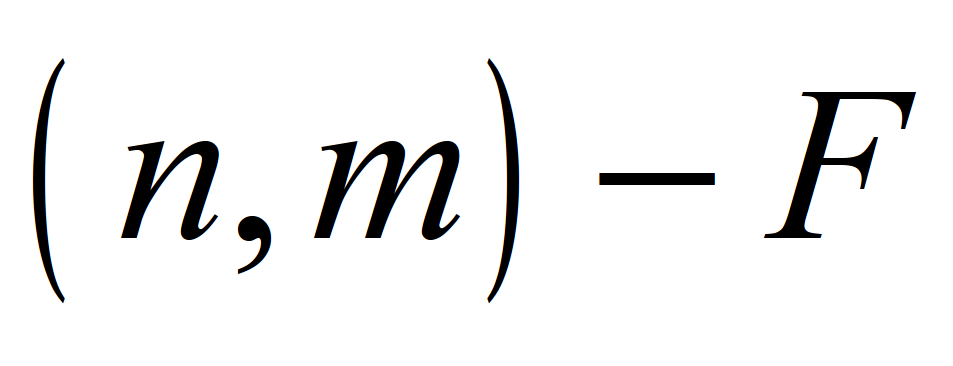
\includegraphics[width=0.8417in,height=0.3346in]{crypt-img/crypt-img81.png} 
називається відображення, яке можна зобразити наступними способами:

а) $(n,m)-F:Z_2^n \to Z_2^{m};$

б)  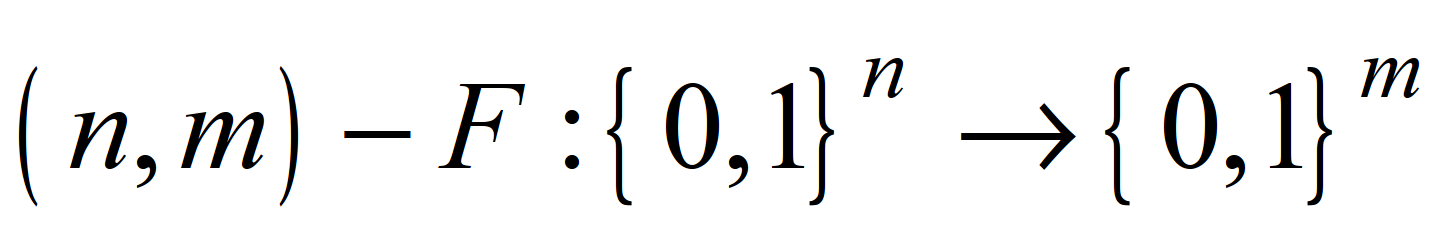
\includegraphics[width=2.2756in,height=0.3854in]{crypt-img/crypt-img82.png}
;

в)  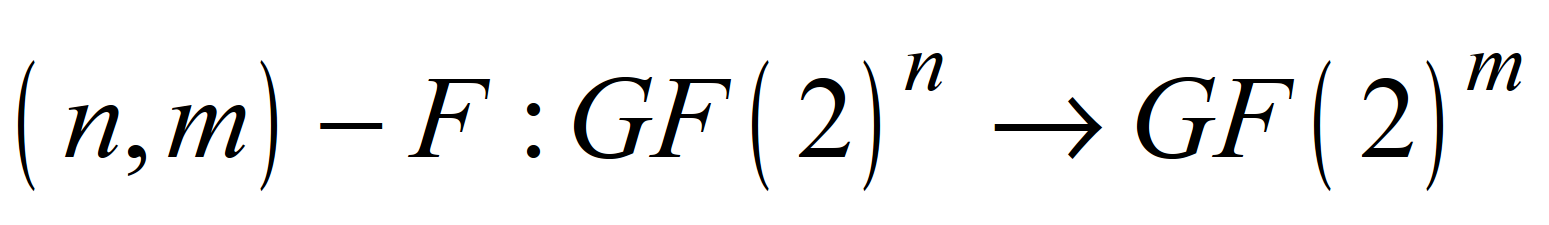
\includegraphics[width=2.6339in,height=0.3862in]{crypt-img/crypt-img83.png}
; $ $

г)  ($n$$,$$m$)\textit{{}-$F$\textit{:}
$V_n \to V_m;$

де $n$, \textit{m }--- розмірності вхідного і вихідного векторів
відповідно. 

Тобто аргументом функції є булевий $n$-вектор, координати якого ,,0'' та
,,1'',  а значенням функції є булевий $m$-вектор. 
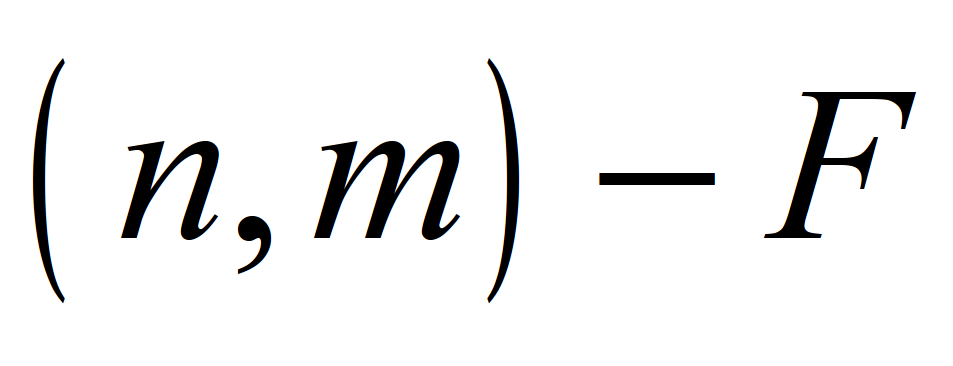
\includegraphics[width=0.8417in,height=0.3346in]{crypt-img/crypt-img84.png} 
розглядають також як функцію від $n$ булевих змінних. Представимо 
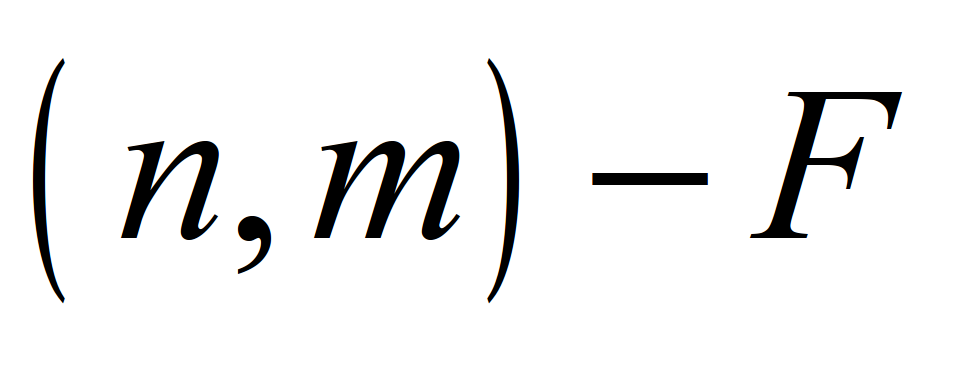
\includegraphics[width=0.8618in,height=0.3354in]{crypt-img/crypt-img85.png}  у
вигляді   $(n,m)-F=(f_1,\dots,f_m)$ ,  де функції
$f$ $_i$\textit{=}
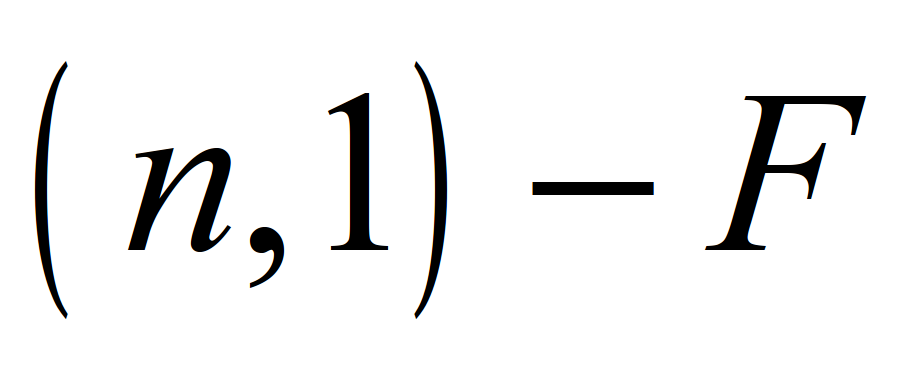
\includegraphics[width=0.7709in,height=0.3335in]{crypt-img/crypt-img86.png} , 
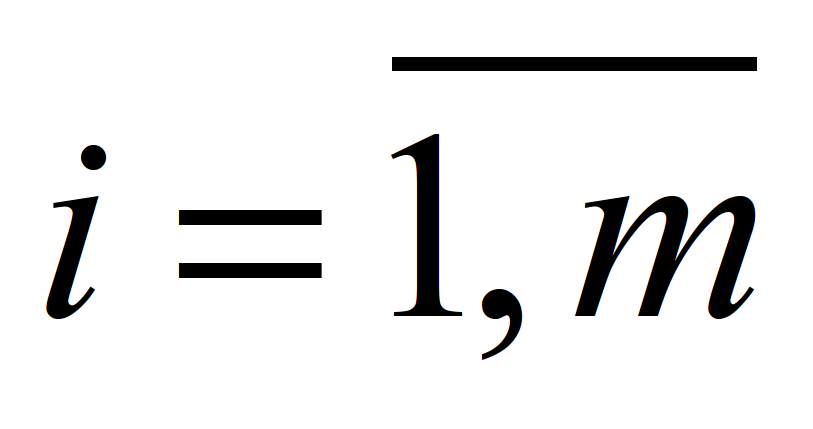
\includegraphics[width=0.6457in,height=0.3327in]{crypt-img/crypt-img87.png} , ---
одновимірні  булеві функції, які називаються координатними функціями. Будемо
позначати 
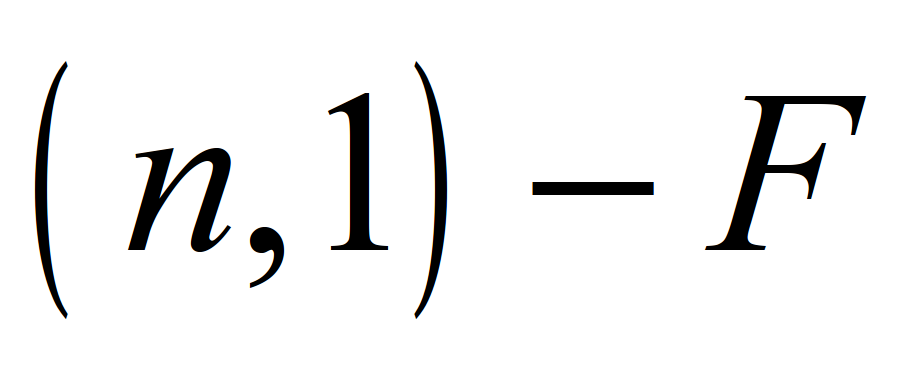
\includegraphics[width=0.7752in,height=0.3354in]{crypt-img/crypt-img88.png} 
через  
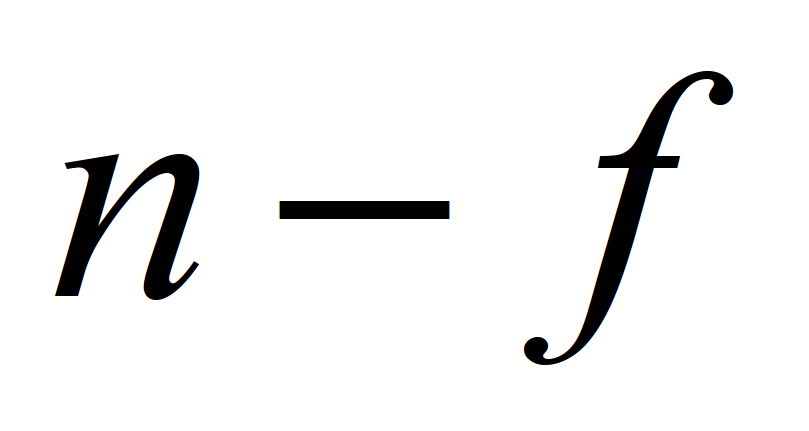
\includegraphics[width=0.5102in,height=0.2709in]{crypt-img/crypt-img89.png}  ,
або просто $f$, якщо з контексту ясно, що це булева функція від
$n$ змінних. 

Нехай 
\includegraphics[width=0.3118in,height=0.3335in]{crypt-img/crypt-img90.png}  ---
множина всіх 
\includegraphics[width=0.8811in,height=0.3339in]{crypt-img/crypt-img91.png} 
функцій; 
\includegraphics[width=0.2984in,height=0.2984in]{crypt-img/crypt-img92.png}  ---
множина всіх булевих функцій вигляду  
\includegraphics[width=0.7866in,height=0.3346in]{crypt-img/crypt-img93.png} ,
тобто булевих функцій від \textit{n }змінних, що приймають значення 0 або 1.
Дуже важлива оцінка кількості  булевих функцій, а також числа функцій зі
спеціальними властивостями. Наведемо деякі необхідні комбінаторні твердження.

$\blacklozenge$ \textit{Декартовим добутком}  $A\times B$, де
\textit{А}і $B$ --- довільні скінченні
множини, називається множина всіх впорядкованих пар 
$\left(a_i},b_j\right)$, де  $a_i}\in A,\ b_j\in B$. 
Декартовий добуток  $n$ множин визначається як множина всіх різних
впорядкованих наборів з $n$елементів, в кожному з яких 
$j$-ий елемент належить $j$-ій  множині.

$\blacklozenge$ \textit{Кардинальним степенем }
$А}^{\text{В}=\left\{\;\varphi :\;B\rightarrow A\;\right\$, де
\textit{А }і \textit{B } --- довільні скінченні множини, називається
множина всіх відображень з множини \textit{В} у множину  \textit{А. } 

\textit{Твердження 9.1} (без доведення). Для потужності декартового добутку
множин маємо співвідношення 

 $|A_1\times A_2\times \dots\times
A_n|=|A_1|\times |A_2|\times \dots\times
|A_n|$,   $|A^n|=|A|^n$


\bigskip

\textit{Твердження 9.2} (без доведення).Потужність множини всіх
відображень з   $B$в $A$  через потужності  множин 
\textit{А  }і  \textit{В}  можна знайти за формулою  
\includegraphics[width=0.9354in,height=0.4055in]{crypt-img/crypt-img94.png} . 

\textit{Твердження 9.3. }Кількість всіх функцій 
\includegraphics[width=0.8508in,height=0.3346in]{crypt-img/crypt-img95.png} 
дорівнює 

$$

\textlatin{[F034?]}\textit{Доведення} 

Розглянемо множину всіх відображень виду 
\includegraphics[width=2.1925in,height=0.3583in]{crypt-img/crypt-img97.png} 
(кардинальний степінь), тоді згідно з твердженнями 9.1 та 9.2

$$ \includegraphics[width=4.7756in,height=0.7402in]{crypt-img/crypt-img98.png}
.\textlatin{[F033?]}
\par}


\bigskip


\bigskip


\bigskip

\textit{Твердження 9.4}  Кількість  всіх одновимірних булевих функцій від
\textit{n }змінних дорівнює  
\includegraphics[width=0.8339in,height=0.4016in]{crypt-img/crypt-img99.png} .

\textlatin{[F034?]}Прямий наслідок з твердження 9.3 при  $m$\textit{ =
}1.\textlatin{[F033?]}


\bigskip


\bigskip

\section{Способи завдання булевих функцій}


\bigskip

Опишемо найбільш поширені і важливі в криптографії способи завдання булевих
функцій.


\bigskip

\liststyleWWviiiNumlii
\begin{enumerate}
\item \textbf{\textit{Таблиця істинності}} \textbf{\textit{для 
(}}\textbf{$n$}\textbf{$,$}\textbf{$m$}\textbf{\textit{)-}}\textbf{$F$}\textbf{\textit{
 функції}}
\end{enumerate}
 (див. рис. 9.1, 
\includegraphics[width=0.8189in,height=0.3189in]{crypt-img/crypt-img100.png} ).


\bigskip



\begin{figure}
\centering
\includegraphics[width=5.0043in,height=2.5457in]{crypt-img/crypt-img101.png}
\end{figure}

\bigskip


\bigskip


\bigskip


\bigskip


\bigskip


\bigskip


\bigskip


\bigskip


\bigskip


\bigskip


\bigskip


\bigskip

У лівій колонці таблиці істинності записані усі можливі набори змінних, проти
кожного набору в правій --- значення функції ( булевий   $m$-вектор). Дві
функції будуть різними, якщо в правій колонці хоча б два біти  
\includegraphics[width=0.9335in,height=0.3618in]{crypt-img/crypt-img102.png}  в
одній і тій самій позиції не однакові. Таким чином, кількість різних функцій
дорівнює числу різних наборів з ,,0'' та ,,1''  на   $\mathit{m2}^n$ місцях у
правій колонці, тобто   $2^{\mathit{m2}^{n}$, що співпадає з твердженням
 9.3.


\bigskip

\liststyleWWviiiNumlii
\setcounter{saveenum}{\value{enumi}}
\begin{enumerate}
\setcounter{enumi}{\value{saveenum}}
\item {\bfseries\itshape
Булеві формули (набір формул)}
\end{enumerate}
Нехай 
\includegraphics[width=1.3854in,height=0.3465in]{crypt-img/crypt-img103.png} 
деяка множина булевих функцій, яку будемо називати  базисом. Формулами в базисі
 \textit{G  }називаються наступні вирази:

\liststyleWWviiiNumv
\begin{enumerate}
\item Будь-яка змінна  $x_i$ є формула;
\item Якщо 
\includegraphics[width=0.7717in,height=0.2984in]{crypt-img/crypt-img104.png}  ---
формули,  $g_i}\in G$, то 
\includegraphics[width=1.1811in,height=0.3465in]{crypt-img/crypt-img105.png}  ---
теж формула;
\item Інших формул, окрім заданих виразами 1) і 2), в заданому базисі немає.
\end{enumerate}
Наприклад, формулами  можуть бути формули алгебри логіки  у базисі  
$G=\left\{x\vee y,\;x\wedge y,\;\;\overset{?}{x}\;\right\$. 

\textit{Твердження 9.5 }Будь-яка функція 
\includegraphics[width=0.6244in,height=0.3016in]{crypt-img/crypt-img106.png} 
зображається у вигляді

$$

де  \includegraphics[width=1.0583in,height=0.3307in]{crypt-img/crypt-img108.png}
,  \includegraphics[width=1.4165in,height=0.6354in]{crypt-img/crypt-img109.png}
. Такий запис називається  розкладом за першими $k$змінними.

\textlatin{[F034?]}\textit{Доведення} 

Згідно з означенням   $1^{0}=0,\;1^{1}=1,\;0^{0}=1,\;0^{1}=0$, тобто 
$x^{x}=1,\;x^{\overset{{?}{x}}}=0$. Звідси випливає, що 
\includegraphics[width=1.339in,height=0.35in]{crypt-img/crypt-img110.png}  тоді
і тільки тоді, коли  $\sigma _i}=x_i\ }\forall i$ та в диз’юнкції
залишиться тільки один відповідний доданок, що спричиняє  за собою  рівність в
твердженні.

Очевидно, можливо записати розклад за будь-якими змінними.

\textit{Твердження 9.6}\textbf{  }Будь-яка функція 
\includegraphics[width=0.6354in,height=0.3016in]{crypt-img/crypt-img111.png} 
може бути зображена у досконалій диз'юнктивній нормальній
формі (ДДНФ) і притому єдиним чином:

$$

 Це твердження  {}- безпосередній наслідок твердження  9.5при 
$k$=\textit{ $n$\textit{.}

$\blacklozenge$ Для фіксованих 
\includegraphics[width=0.6571in,height=0.248in]{crypt-img/crypt-img113.png} 
для запису 
\includegraphics[width=2.0201in,height=0.3346in]{crypt-img/crypt-img114.png} 
вводять позначення 
\includegraphics[width=1.7398in,height=0.3535in]{crypt-img/crypt-img115.png} , 
яке називається підфункцією від  
\includegraphics[width=0.4681in,height=0.2409in]{crypt-img/crypt-img116.png} 
змінних. Аналогічні позначення і для підфункції будь-яких (не обов’язково
перших) 
\includegraphics[width=0.4681in,height=0.2409in]{crypt-img/crypt-img117.png}
змінних. 


\bigskip

\liststyleWWviiiNumlii
\begin{enumerate}
\item {\bfseries\itshape
Поліном Жегалкіна (алгебраїчна  нормальна форма)}
\end{enumerate}
 \begin{definition}
\textit{9.}\textit{2.}Поліномом Жегалкіна від
$n$ змінних називається канонічний многочлен над полем \textit{GF(2)
}виду

$$

де коефіцієнти   $a_0,a_i_{{1}\dotsi_k}}\in
\left\{0,1\right\}$, обидві суми --- булеві ( в полі \textit{GF(2)}), друге
сумування --- по всіх невпорядкованих наборах  індексів 
$i_1,\dots,i_k$

\textit{Твердження 9.7}  Будь-яка функція 
$f(x_1,\dots,x_n)$ може бути зображена у вигляді
полінома Жегалкіна, причому єдиним чином.

\textlatin{[F034?]}Доведення. Зауважимо, що 

$$ \includegraphics[width=0.728in,height=0.2161in]{crypt-img/crypt-img119.png}
\textbf{, }
\includegraphics[width=3.4709in,height=0.3228in]{crypt-img/crypt-img120.png}
\textbf{,  } $$

Тут відповідні функції в лівій частині рівностей записані за допомогою логічних
операцій, а в правій --- операціями в полі  \textit{GF(2).} Згідно твердженню
9.6запишемобулеву функцію як ДДНФ. Перетворивши таке
зображення за допомогою співвідношень із зауваження, розкривши дужки, звівши
подібні доданки, спростивши вираз  в полі \textit{GF(2)}\textit{, }одержимо
поліном Жегалкіна. Таким чином, немає булевих функцій, які неможливо було б
представити у вигляді полінома Жегалкіна.

Доведемо єдиність такого зображення. Кількість можливих поліномів Жегалкіна не
більше числа всіх можливих наборів значень коефіцієнтів 
\includegraphics[width=0.8154in,height=0.3307in]{crypt-img/crypt-img121.png} .
У кожному розкладі виду

{\centering 
\includegraphics[width=3.8752in,height=0.6661in]{crypt-img/crypt-img122.png}
\par}

присутні 
\includegraphics[width=2.5201in,height=0.3646in]{crypt-img/crypt-img123.png} 
коефіцієнтів, які можуть приймати значення або 0, або 1, отже, число можливих
наборів значень коефіцієнтів 
\includegraphics[width=0.7472in,height=0.3071in]{crypt-img/crypt-img124.png} 
дорівнює 
\includegraphics[width=0.3264in,height=0.3264in]{crypt-img/crypt-img125.png} .
Це число співпадає з потужністю множини 
\includegraphics[width=0.8339in,height=0.4016in]{crypt-img/crypt-img126.png} ,
що і доводить єдність зображення, оскільки якщо  хоча б одна функція мала два
різні поліноми Жегалкіна, то існувала б функція, що не має такого полінома, що
суперечить вище доведеному.\textlatin{[F033?]}

\textit{Означення 9.3.} Алгебраїчним степенем 
\includegraphics[width=0.5425in,height=0.2665in]{crypt-img/crypt-img127.png} 
булевої функції 
\includegraphics[width=0.9098in,height=0.3354in]{crypt-img/crypt-img128.png} 
називається максимальний степінь доданків з ненульовими коефіцієнтами в
зображенні функції поліномом Жегалкіна. Під степенем доданка розуміється число
невідомих, що в нього входять. Наприклад, лінійні булеві функції мають степінь,
що дорівнює 1, або є константами; степінь функції 
\includegraphics[width=2.248in,height=0.3583in]{crypt-img/crypt-img129.png}  
дорівнює  2. Максимальний степінь булевої функції від $n$ змінних
дорівнює $n$.


\bigskip

\liststyleWWviiiNumlii
\setcounter{saveenum}{\value{enumi}}
\begin{enumerate}
\setcounter{enumi}{\value{saveenum}}
\item {\bfseries\itshape
Розклад (ряд) Фур’є }
\end{enumerate}
\textit{Твердження 9.8 }Сімейство функцій 
\includegraphics[width=0.8181in,height=0.3661in]{crypt-img/crypt-img130.png} , 
$a\in \left\{0,1\right\}^n$, кожна з яких є  булевою функцією від
$n$ булевих змінних, ортогональне:

{\centering 
\includegraphics[width=3in,height=0.75in]{crypt-img/crypt-img131.png} \par}

де  \includegraphics[width=1.0071in,height=0.3827in]{crypt-img/crypt-img132.png}
 --- довільні булеві $n$-вектори, 
\includegraphics[width=0.5071in,height=0.3354in]{crypt-img/crypt-img133.png}  ---
скалярний добуток $n$-векторів над полем \textit{GF(2)}, 
\includegraphics[width=0.8508in,height=0.3866in]{crypt-img/crypt-img134.png} ,
а підсумовування відбувається в дійсній області.

\textlatin{[F034?]}\textit{Доведення}

 Будь-яка лінійна, не рівна тотожно  нулю  або одиниці функція ,,рівноімовірно''
приймає значення 0 і 1, тобто в правій частині таблиці істинності міститься
однакова кількість нулів і одиниць. Дійсно, розглянемо деяку істотну змінну 
\includegraphics[width=0.228in,height=0.2744in]{crypt-img/crypt-img135.png}  (а
така існує, бо функція не є константою):

$$

При 
\includegraphics[width=0.2319in,height=0.2709in]{crypt-img/crypt-img137.png} 
рівному 0 або 1 значення функції буде відповідно  0 або 1, чи навпаки   1 або 0
 залежно від значення решти змінних, тобто при будь-якому наборі решти змінних
функція приймає як  значення  0 так і значення 1. Це й означає, що в правій
частині таблиці істинності міститься рівна кількість нулів і одиниць.

Далі маємо: скалярний добуток 
\includegraphics[width=0.4681in,height=0.3055in]{crypt-img/crypt-img138.png} ,
де 
\includegraphics[width=1.1535in,height=0.3075in]{crypt-img/crypt-img139.png} ,
--- лінійна булева функція,  
\includegraphics[width=0.4953in,height=0.2862in]{crypt-img/crypt-img140.png} 
та 
\includegraphics[width=0.6811in,height=0.2917in]{crypt-img/crypt-img141.png} ,

$$

де  \includegraphics[width=0.5043in,height=0.2634in]{crypt-img/crypt-img143.png}
 --- порозрядна булева сума векторів. Якщо 
\includegraphics[width=0.4898in,height=0.25in]{crypt-img/crypt-img144.png} , то
 \includegraphics[width=0.8126in,height=0.3335in]{crypt-img/crypt-img145.png} 
--- не рівна тотожно нулю рівноймовірна функція, значить серед доданків суми
присутня однакова кількість як 1, так і -1, тобто сума тотожно рівна нулю. Якщо
ж  \includegraphics[width=0.472in,height=0.2508in]{crypt-img/crypt-img146.png}
, то 
\includegraphics[width=1.0866in,height=0.3307in]{crypt-img/crypt-img147.png} , 
отже всі 
\includegraphics[width=0.2516in,height=0.2917in]{crypt-img/crypt-img148.png}
доданків  суми ,,1''  і сума дорівнюють 
\includegraphics[width=0.2516in,height=0.2957in]{crypt-img/crypt-img149.png}
.\textlatin{[F033?]}

\textit{Твердження 9.9  }Будь-яка функція 
\includegraphics[width=0.6252in,height=0.3016in]{crypt-img/crypt-img150.png} 
може бути зображена у вигляді

$$ \includegraphics[width=2.5626in,height=0.6335in]{crypt-img/crypt-img151.png} , 
 \includegraphics[width=2.3154in,height=0.6689in]{crypt-img/crypt-img152.png} ,
\par}

причому єдиним чином. Підсумовування тут відбувається в дійсній області.
Коефіцієнти  $с_{\alpha $ називаються коефіцієнтами Фур’є, а дане
зображення ---\textcolor{red}{ }рядом  або розкладом Фур’є.

\textlatin{[F034?]}\textit{Доведення.} 

Якщо коефіцієнти  $с_{\alpha $ мають наведений у твердженні вигляд,
то для будь-якого фіксованого 
\includegraphics[width=0.6055in,height=0.3382in]{crypt-img/crypt-img153.png}  
і довільної функції 
\includegraphics[width=0.4689in,height=0.3228in]{crypt-img/crypt-img154.png}
\textbf{ }від\textbf{ $n$змінних отримаємо:

{\centering 
\includegraphics[width=6.3654in,height=0.7362in]{crypt-img/crypt-img155.png}
\par}

 \includegraphics[width=2.0634in,height=0.5854in]{crypt-img/crypt-img156.png} . 
Тобто результат перетворення Фур’є --- значення функції від аргументу 
\includegraphics[width=0.6102in,height=0.339in]{crypt-img/crypt-img157.png} .

Доведемо єдиність розкладу. Нехай функція 
\includegraphics[width=0.4453in,height=0.3102in]{crypt-img/crypt-img158.png} 
має два розклади з наборами коефіцієнтів 
\includegraphics[width=0.2709in,height=0.2709in]{crypt-img/crypt-img159.png}  і
 \includegraphics[width=0.2709in,height=0.2709in]{crypt-img/crypt-img160.png} .
Віднімемо ці два розклади:

$$

Помноживши  обидві частини на 
\includegraphics[width=0.6528in,height=0.3193in]{crypt-img/crypt-img162.png}  і
 підсумувавши  по $x$, одержуємо 

{\centering 
\includegraphics[width=5.5811in,height=0.6563in]{crypt-img/crypt-img163.png}
\par}

За твердженням 9.8 друга сума дорівнює нулю, коли  $\alpha \neq \beta $,  та  
\includegraphics[width=0.2516in,height=0.2957in]{crypt-img/crypt-img164.png} ,
коли  $\alpha =\beta $. Таким чином, у перший сумі буде тільки один
ненульовий доданок при  $\alpha =\beta $. Звідки випливає, що

 \includegraphics[width=1.8071in,height=0.3661in]{crypt-img/crypt-img165.png} ,
тобто  
\includegraphics[width=1.1366in,height=0.2866in]{crypt-img/crypt-img166.png}
.\textlatin{[F033?]}


\bigskip

\liststyleWWviiiNumlii
\setcounter{saveenum}{\value{enumi}}
\begin{enumerate}
\setcounter{enumi}{\value{saveenum}}
\item \textbf{\textit{Перетворення  Уолша}}\textbf{$$-}
\textbf{\textit{Адамара}}\textbf{\textit{.}}
\end{enumerate}
 \begin{definition}
\textit{9.}\textit{4}Перетворенням Уолша-Адамара
називається функція 

$$H_f(\alpha )=\underset{x\in Z_{{2}^n}}{\sum
}{(-1)^{f(x){\oplus}(x,\alpha )}}$$

де підсумовування відбувається в дійсній області. Для будь-якого  $\alpha $
значення  $H_f(\alpha )$ називається коефіцієнтом Уолша-Адамара, 
$\underset{\alpha }{max}|H_f(\alpha )|\le 2^{n/2$

Будь-яка функція 
\includegraphics[width=0.6102in,height=0.2819in]{crypt-img/crypt-img167.png} 
може бути зображена через перетворення Уолша-Адамара за формулою обертання


\bigskip

$$(-1)^{f(x)}=2^{-n}\underset{\alpha \in Z_{{2}^n}}{\sum
}{H_f(\alpha )(-1)^{(x,\alpha )}}$$

причому єдиним чином.

Коефіцієнти Фур’є та Уолша-Адамара зв’язані співвідношенням


\bigskip

$$

де дельта-функція   $\delta (\alpha
)=?\begin{matrix}\left\{1,\;\;якщо\;\alpha
=0?\right\}\left\{0,\;якщо\;\alpha \neq
0?\right.\mathit{rbra}\end{matrix}\{\}$


\bigskip

\liststyleWWviiiNumlii
\setcounter{saveenum}{\value{enumi}}
\begin{enumerate}
\setcounter{enumi}{\value{saveenum}}
\item {\bfseries\itshape
Про інші способи завдання булевих функцій.}
\end{enumerate}
 Окрім наведених способів завдання булевих функцій, існують інші: алгоритмічне,
завдання контактними (рис. 9.2), функціональними схемами, завдання за допомогою
вершин одиничного \textit{n-}вимірногокуба, набором відстаней до усіх
лінійних функцій ( див. лекцію 10)  тощо.


\bigskip



\begin{figure}
\centering
\begin{minipage}{2.4217in}
{\centering 
\includegraphics[width=1.802in,height=0.9374in]{crypt-img/crypt-img168.png}
\par}
\end{minipage}
\end{figure}

\bigskip


\bigskip


\bigskip


\bigskip

[Warning: Draw object ignored]

$$


\bigskip


\bigskip

\section{Контрольні питання }


\bigskip


\bigskip

\liststyleWWviiiNumlvii
\begin{enumerate}
\item Яку роль\textbf{ }відіграють булеві функції в криптографії?
\item Дайте визначення булевої функції та багатовимірної булевої функції.
\item Що таке таблиця істиності булевої функції?
\item Запишіть ДДНФ для булевої функції від $n$ змінних.
\item Наведіть означення полінома Жегалкіна і алгебраїчного
с\textcolor[rgb]{0.0,0.5019608,0.0}{тепеня}  булевої функції.
\item Скільки доданків у поліномі Жегалкіна, якщо усі його коефіцієнти не
дорівнюють нулю?
\item Чим відрізняються розклад Фур’є і перетворення Уолша?
\item Які Ви знаєте інші способи завдання булевих функцій?
\end{enumerate}

\bigskip


\bigskip


\bigskip


\bigskip


\bigskip


\bigskip


\bigskip


\bigskip

{\bfseries
ЛЕКЦІЯ  10}


\bigskip

{\centering\bfseries
СКЛАДНІСТЬ БУЛЕВИХ ФУНКЦІЙ.
\par}

{\centering\bfseries
КЛАСИ  І  КРИПТОГРАФІЧНІ ВЛАСТИВОСТІ БУЛЕВИХ ФУНКЦІЙ
\par}


\bigskip


\bigskip

Визначення криптографічних характеристик булевих функцій, критеріїв, яким вони
повинні задовольняти, складності їх реалізації,  підрахунок  числа функцій, що
мають певні властивості, методи синтеза, генерації булевих функцій з необхідним
набором криптографічних характеристик --- все це має першорядне значення для
побудови надійних, стійких криптосистем.


\bigskip


\bigskip

\section{Складність булевих функцій}


\bigskip


\bigskip

Будемо говорити, що властивість Р виконується майже для всіх булевих функцій 
\includegraphics[width=0.6311in,height=0.2972in]{crypt-img/crypt-img169.png} ,
якщо  $\lim_{n \to \infty}\frac{|\Omega
_n^{p}|}{|\Omega _n|}=1$, де  $ $ $|\Omega _n^{p}|$ -
потужність множини  $\Omega _n^{p$ булевих функцій від $n$
змінних, для яких виконується властивість Р.

Позначимо wt\textit{($f$\textit{)} (або  wt $f$\textit{ 
})вагу булевої  функції 
\includegraphics[width=0.528in,height=0.25in]{crypt-img/crypt-img170.png}  -
число одиниць в правій колонці таблиці істинності. Вагою wt $\alpha $
булевого вектора  $\alpha =(\alpha _1,\dots,\alpha
_n)$ , будемо називати  $\oversetn{\sum_{1}}{\alpha
_i}}$, тобто число одиниць у векторі.

Для майже всіх булевих функцій 
\includegraphics[width=0.611in,height=0.2874in]{crypt-img/crypt-img171.png} 
(тобто асимптотично у наведеному вище розумінні) виконуються співвідношення:

\liststyleWWviiiNumvi
\begin{enumerate}
\item 
\includegraphics[width=2.7366in,height=0.5008in]{crypt-img/crypt-img172.png} ;
\item Число 
\includegraphics[width=0.3819in,height=0.2945in]{crypt-img/crypt-img173.png} 
доданків в диз'юнктивній нормальній формі (довжина ДНФ)
задовольняє нерівності:
\end{enumerate}
$$ \includegraphics[width=1.8701in,height=0.6311in]{crypt-img/crypt-img174.png} , 
\includegraphics[width=0.8083in,height=0.2071in]{crypt-img/crypt-img175.png} .
\par}

\liststyleWWviiiNumvi
\setcounter{saveenum}{\value{enumi}}
\begin{enumerate}
\setcounter{enumi}{\value{saveenum}}
\item Число контактів в реалізації булевої функції \textit{f }контактною схемою
визначається асимптотичним співвідношенням
\end{enumerate}
$$

Наведені приклади мір складності булевих функцій дають уявлення про складність
реалізації для ,,майже всіх'' булевих функцій апаратними або програмними
способами, автоматичними пристроями (в тому числі електронними). Час роботи
такого пристрою або число елементів у ньому  оцінюється вказаними
співвідношеннями з деякими множниками, що поліноміально залежать від числа
змінних $n$\textit{.} Тобто ,,майже для всіх'' булевих функцій складність
їх реалізації зростає експоненційно з ростом кількості змінних. Наприклад, для 
$n\ge \text{40$ переважна більшість функцій не може бути реалізована
доступними на сьогодні засобами. Блокові шифратори DES, ГОСТ 28147-89 (див.
лекції 12,13) при шифруванні одного блоку ВТ реалізують функції вигляду (64,
64)-$F$\textit{, }переважна більшість яких занадто складна для
практичної реалізації. Очевидно, якщо вибирати функцію випадково, то для
генерування майже всіх булевих функцій потрібно випадково вибрати експоненційно
велику кількість параметрів. Тому для побудови та вибору булевих функцій, що
використовуються у криптографії, необхідно ставитися вкрай ретельно.


\bigskip


\bigskip

\section{Класифікація булевих функцій}


\bigskip


\bigskip

\begin{flushleft}
\tablehead{}
\begin{supertabular}{|m{5.23726in}|m{1.1122599in}|}
\hline
\centering Визначення класу булевої функції &
Позначення класу\\\hline
$\blacklozenge$ Булева функція 
\includegraphics[width=1.25in,height=0.278in]{crypt-img/crypt-img177.png} 
називається\textcolor{red}{ } зберігаючою  нуль, якщо 
\includegraphics[width=1in,height=0.278in]{crypt-img/crypt-img178.png} . &
\centering\arraybslash 
\includegraphics[width=0.1937in,height=0.25in]{crypt-img/crypt-img179.png}
\\\hline
$\blacklozenge$ Булева функція 
\includegraphics[width=1.25in,height=0.278in]{crypt-img/crypt-img180.png} 
називається зберігаючою  одиницю, якщо 
\includegraphics[width=0.9028in,height=0.278in]{crypt-img/crypt-img181.png} . &
\centering\arraybslash 
\includegraphics[width=0.1665in,height=0.25in]{crypt-img/crypt-img182.png}
\\\hline
$\blacklozenge$ Булева функція 
\includegraphics[width=1.25in,height=0.278in]{crypt-img/crypt-img183.png} 
називається самодвоїстою, якщо 
\includegraphics[width=1.889in,height=0.278in]{crypt-img/crypt-img184.png} . &
\centering\arraybslash \itshape S\\\hline
$\blacklozenge$ Булева функція 
\includegraphics[width=1.25in,height=0.278in]{crypt-img/crypt-img185.png} 
називається монотонною, якщо 
\includegraphics[width=1.972in,height=0.278in]{crypt-img/crypt-img186.png}  при
 \includegraphics[width=0.5138in,height=0.25in]{crypt-img/crypt-img187.png} , 
\includegraphics[width=0.4583in,height=0.2638in]{crypt-img/crypt-img188.png} .
&
\centering\arraybslash \itshape М\\\hline
$\blacklozenge$ Булева функція 
\includegraphics[width=1.25in,height=0.278in]{crypt-img/crypt-img189.png} 
називається лінійною, якщо вона  може бути зображена у вигляді 
\includegraphics[width=2.5in,height=0.278in]{crypt-img/crypt-img190.png} , 
$\alpha _i}\in \left\{0,\;1\right\},\;\;i=0,1,\dots,n$
&
\centering\arraybslash 
\includegraphics[width=0.2083in,height=0.25in]{crypt-img/crypt-img191.png}
\\\hline
\end{supertabular}
\end{flushleft}

\bigskip

\textit{Означення 10.1} Система функцій  
\includegraphics[width=1.3854in,height=0.3465in]{crypt-img/crypt-img192.png}
називається \textit{функціонально повною},  якщо будь-яка булева функція може
бути записана у вигляді формули через функції цієї системи (базис).

\textit{Твердження10.1.} Система функцій повна тоді і тільки тоді, коли вона не
є підсистемою жодного з перелічених п’яти класів.

Наприклад, будь-яка булева функція може бути записана за допомогою логічних
функцій доповнення, диз’юнкції та кон’юнкції (див. лекцію 9). Властивості
функцій цих класів, особливо лінійних і монотонних, активно використовуються
при синтезі та аналізі криптографічних перетворень. 

Існують також інші класифікації булевих функцій, що враховують різні властивості
булевих функцій. Наприклад: розбиття усіх булевих функцій на класи ,,однаково
мінімізуємих `` функцій, класифікація за геометричною схожістю, виділення
інваріантних класів, що тісно пов’язані зі схемною реалізацією тощо. У даній та
наступній лекціях ми розглянемо найбільш важливі класи булевих функцій, що
мають криптографічні властивості, необхідні для побудови надійних
криптографічних перетворень.


\bigskip

\section{Криптографічні властивості булевих функцій}


\bigskip


\bigskip

\liststyleWWviiiNumxxix
\begin{enumerate}
\item {\bfseries\itshape
Невиродженість}
\end{enumerate}
 \textit{Означення10.2.}Змінна  
\includegraphics[width=0.2083in,height=0.25in]{crypt-img/crypt-img193.png} 
називається  істотною для булевої функції 
\textit{($n$$,$$m$\textit{)-$F$, якщо існує набір
 \includegraphics[width=1.7362in,height=0.278in]{crypt-img/crypt-img194.png} , 
\includegraphics[width=0.6937in,height=0.278in]{crypt-img/crypt-img195.png} 
такий, що 

\begin{equation*}
{F(\alpha _1,\dots,\alpha _{k-1},0,\alpha
_{k+1},\dots,\alpha _n)\neq F(\alpha
_1,\dots,\alpha _{k-1},1,\alpha
_{k+1},\dots,\alpha _n)}
\end{equation*}
 \textit{Означення10.3.}Булева функція
\textit{($n$$,$$m$\textit{)-$F$  називається
невиродженою, якщо всі її змінні істотні.

Якщо функція вироджена, то вона має фіктивні змінні, що не впливають ніколи на
значення функції та можуть дати нагоду для криптоаналізу, складність функції
буде відповідно менше. Більш сильною вимогою для функції є наступне означення.

 \textit{Означення10.4.}Булева функція
\textit{($n$$,$$m$\textit{)-$F$  називається
невиродженою, якщо всі її змінні істотні для кожної з $n$ координатних
\textit{($n$$,$1\textit{)-$F$  функцій.

Ця властивість стверджує, що кожен біт входу булевої функції має вплив на кожний
біт виходу.


\bigskip

\liststyleWWviiiNumxxix
\setcounter{saveenum}{\value{enumi}}
\begin{enumerate}
\setcounter{enumi}{\value{saveenum}}
\item {\bfseries\itshape
Рівноймовірність (збалансованість)}
\end{enumerate}
 \textit{Означення10.5.}Булева функція 
\includegraphics[width=0.8744in,height=0.3425in]{crypt-img/crypt-img196.png} 
називається рівноймовірною (збалансованою), якщо 

$$

де   $|F^{-1}(y)|$ - кількість прообразів вектора  $y$.

Зокрема, функція $n$\textit{{}-$f$ рівноймовірна тоді і тільки
тоді, коли 
\includegraphics[width=0.8193in,height=0.278in]{crypt-img/crypt-img198.png} .

\textit{Означення10.6.}Булева функція
\textit{($n$$,$$m$\textit{)-$F$  називається
$k$\textit{{}-}рівноймовірною або $k$\textit{{}-}збалансованою,
якщо 
\includegraphics[width=0.611in,height=0.278in]{crypt-img/crypt-img199.png}  
\includegraphics[width=0.75in,height=0.278in]{crypt-img/crypt-img200.png}  
$(\forall (\alpha _i_{{1}}},\dots,\alpha _i_t}{)\in
\left\{0,\;1\right\}^{t}}{\;)}$  підфункція від 
\includegraphics[width=0.3465in,height=0.1665in]{crypt-img/crypt-img201.png} 
змінних, одержана фіксацією змінних 
\includegraphics[width=1.389in,height=0.278in]{crypt-img/crypt-img202.png} ,
буде рівноймовірною.  

\textit{Твердження 10.2}\textit{. }Булева функція 
\includegraphics[width=0.528in,height=0.25in]{crypt-img/crypt-img203.png}  є
$k$-рівноймовірноютоді і тільки тоді, коли коефіцієнти в
розкладі її в ряд Фур’є такі:

$$ \includegraphics[width=0.5138in,height=0.4307in]{crypt-img/crypt-img204.png} , 
 \includegraphics[width=0.5138in,height=0.25in]{crypt-img/crypt-img205.png} 
для всіх  $\alpha $таких, що 
\includegraphics[width=0.611in,height=0.1937in]{crypt-img/crypt-img206.png} .
\par}

Приклад $k$-рівноймовірної булевої\textit{
$n$\textit{{}-$f$  функції від $n$змінних: 
$f(x_1,\dots,x_{n-k-1}){\oplus}x_{n-k}{\oplus}\dots{\oplus}x_n$
.

Рівноймовірність надзвичайно важлива криптографічна характеристика. Якщо функція
рівноймовірна, то знання значення функції  (виходу) не дає ніякої додаткової
інформації про значення вхідних змінних.  


\bigskip

\liststyleWWviiiNumxxix
\setcounter{saveenum}{\value{enumi}}
\begin{enumerate}
\setcounter{enumi}{\value{saveenum}}
\item {\bfseries\itshape
Кореляційний імунітет.}
\end{enumerate}
Розглянемо булеву функцію
\textit{($n$$,$$m$\textit{)-$F$  . Задамо на
множині  $2^n$ вхідних векторів $x$ $?$
\includegraphics[width=0.4437in,height=0.3193in]{crypt-img/crypt-img207.png} 
рівноймовірний розподіл. Він індукує деякий імовірнісний розподіл на множині
всіх вихідних векторів $y$ $?$ $\left\{0,\;1\right\}^{m$ для
даної 
\includegraphics[width=0.8744in,height=0.3425in]{crypt-img/crypt-img208.png} 
функції.

 \textit{Означення10.7.}Булева функція
\textit{($n$$,$$m$\textit{)-$F$  має кореляційний
імунітет  \textit{к-го }порядку  $(1\le k\le n)$, якщо 
\includegraphics[width=1.8598in,height=0.3634in]{crypt-img/crypt-img209.png} 
таких, що 
\includegraphics[width=0.5689in,height=0.3272in]{crypt-img/crypt-img210.png} 
\textbf{при }
\includegraphics[width=0.528in,height=0.2701in]{crypt-img/crypt-img211.png} ,
для будь-якої  координати 
\includegraphics[width=0.2898in,height=0.348in]{crypt-img/crypt-img212.png}
\textbf{, }
\includegraphics[width=0.5583in,height=0.2736in]{crypt-img/crypt-img213.png} 
вихідного $m$-вектора  взаємна інформація між випадковим булевим 
вектором  $(x_i_{{1}}},\dots,x_i_k}{)$ і
випадковою булевою величиною  $y_r$ дорівнює нулю:

$$

Підкреслимо, що розглядати відповідні ентропії та взаємну інформацію стало
можливо після того, як на множині  вхідних векторів $x$ $?$
\includegraphics[width=0.4437in,height=0.3193in]{crypt-img/crypt-img214.png} 
було задано ймовірнісний розподіл. Нагадаємо, що взаємна інформація  між
довільними імовірнісними  ансамблями \textit{X }і \textit{У}, тобто між
множинами з імовірнісними мірами можна знайти з формулою

{\centering\itshape
 \includegraphics[width=3.402in,height=0.3744in]{crypt-img/crypt-img215.png} , 
\par}

$$

Існує також комбінаторне визначення кореляційного імунітету.

\textit{Означення10.8.}Булева функція
\textit{($n$$,$$m$\textit{)-$F$  має кореляційний
імунітет (кореляційно імунна) \textit{к-го }порядку, якщо для будь-якого
фіксованого набору індексів 
\includegraphics[width=0.528in,height=0.25in]{crypt-img/crypt-img216.png}  та
будь-якого фіксованого вихідного вектора 
\includegraphics[width=1.0693in,height=0.278in]{crypt-img/crypt-img217.png} 
кожне з можливих  $2^{k$ значень підвектора 
\includegraphics[width=0.8193in,height=0.3335in]{crypt-img/crypt-img218.png}  у
векторах  $x=(x_1,\dots,x_n)$, що належать множині
прообразів вектора 
\includegraphics[width=1.0693in,height=0.278in]{crypt-img/crypt-img219.png}  
(у лівій колонці таблиці істинності функції 
\includegraphics[width=0.8744in,height=0.3425in]{crypt-img/crypt-img220.png} ),
зустрічається однакове число раз.

\textit{Твердження 10.3}Булева функція
\textit{($n$$,$$m$\textit{)-$F$  має кореляційний
імунітет \textit{к-го }порядку, якщо перетворення Адамара-Уолша 
$H_f(\alpha )=\underset{x\in Z_{{2}^n}}{\sum
}{(-1)^{f(x){\oplus}(x,\alpha )}}=0$ для всіх 
\includegraphics[width=0.2083in,height=0.278in]{crypt-img/crypt-img221.png} ,
$j$=1,…,$m$, та   $\alpha $таких, що wt
$\alpha \;\le k$, де 
\includegraphics[width=0.2083in,height=0.278in]{crypt-img/crypt-img222.png}  ---
\textit{j-}а координатна функція.

\textit{Твердження 10.4}Якщо булева $n$\textit{{}-$f$ 
функція  має кореляційний імунітет \textit{к-го }порядку, то 
\includegraphics[width=1.1535in,height=0.272in]{crypt-img/crypt-img223.png} .
Якщо при цьому вона ще й  є рівноімовірною (збалансованою), то 
\includegraphics[width=1.4134in,height=0.272in]{crypt-img/crypt-img224.png} .

Кореляційний імунітет дозволяє уникнути так званої кореляційної атаки, коли
криптоаналітик має можливість знаходити невідомі параметри (наприклад, біти
ключа) по частинах.


\bigskip

\liststyleWWviiiNumxxix
\setcounter{saveenum}{\value{enumi}}
\begin{enumerate}
\setcounter{enumi}{\value{saveenum}}
\item {\bfseries\itshape
Лавинний ефект (розповсюдження помилок)}
\end{enumerate}
Нехай на множині  вхідних векторів  $x\in ?$
\includegraphics[width=0.4437in,height=0.3193in]{crypt-img/crypt-img225.png} 
функції \textit{($n$$,$$m$\textit{)-$F$ , задано
рівномірний розподіл імовірностей:

$$

Тоді імовірнісний розподіл буде задано також на множині всіх вихідних векторів
$y$ $?$ $\left\{0,\;1\right\}^{m$ для цієї 
\textit{($n$$,$$m$\textit{)-$F$  функції.

Введемо позначення: 
\includegraphics[width=0.1528in,height=0.25in]{crypt-img/crypt-img227.png} 
---булевий $n$\textit{{}-} вектор, в якому \textiti-а }компонента рівна
1, а інші рівні 0; 
\includegraphics[width=0.278in,height=0.3193in]{crypt-img/crypt-img228.png}  ---
\textit{j-}акоординатна функція
\textit{($n$$,$$m$\textit{)-$F$  функції,

 \includegraphics[width=2.6528in,height=0.498in]{crypt-img/crypt-img229.png}
---ймовірність того, що $j$-а координатна функція булевої
функції 
\includegraphics[width=1.3555in,height=0.3028in]{crypt-img/crypt-img230.png} 
дорівнює  1.

\textit{ Означення10.9.} Булева 
\textit{($n$$,$$m$\textit{)-$F$  функція має
строгий лавинний ефект нульового порядку, якщо 
\includegraphics[width=2.2874in,height=0.4882in]{crypt-img/crypt-img231.png} .

Еквівалентне визначення:

 \textit{Означення10.10}. Булева
\textit{($n$$,$$m$\textit{)-$F$ функція має
строгий лавинний ефект нульового порядку, якщо 
\includegraphics[width=4.9409in,height=0.7929in]{crypt-img/crypt-img232.png} .

\textit{ Означення10.11.} Булева
\textit{($n$$,$$m$\textit{)-$F$  функція має
строгий лавинний ефект \textit{к-го }порядку, якщо для будь-якого набору
індексів 
\includegraphics[width=0.528in,height=0.25in]{crypt-img/crypt-img233.png} 
кожна підфункція від 
\includegraphics[width=0.4638in,height=0.2374in]{crypt-img/crypt-img234.png} 
змінних, одержана шляхом фіксації змінних  $x_i_{{1}}}=\alpha
_i_1}{,\dots,x_i_k}}{=\alpha _i_k}}$ 
$\forall (\alpha _i_{{1}}},\dots,\alpha _i_k}{)\in
\left\{0,\;1\right\}^{k}}{\;}$, має строгий лавинний ефект нульового порядку. 

Таким чином, строгий лавинний ефект нульового порядку означає, що при зміні
одного біта на вході функції кожний вихідний біт зміниться з ймовірністю рівно
½. Тобто, по будь-яким (навіть мінімальним) змінам на виході функції неможливо
з’ясувати, які зміни відбулися на вході функції, або знайти хоч яку-небудь
характеристику змін.  Більш слабка вимога на властивість розповсюдження помилок
наступна: при зміні одного вхідного біта середня кількість вихідних бітів, що
змінилися, дорівнює $m$\textit{/}2. Для
($n$$,$1)\textit{{}-$F$  функції остання властивість
співпадає зі строгим лавинним ефектом. Лавинний ефект є однією з формальних
характеристик принципу  розповсюдження помилок (розсіювання) Шеннона ( див.
лекцію 7). 


\bigskip

\liststyleWWviiiNumxxix
\setcounter{saveenum}{\value{enumi}}
\begin{enumerate}
\setcounter{enumi}{\value{saveenum}}
\item {\bfseries\itshape
Відсутність заборон на виході}
\end{enumerate}
\textit{ Означення10.12.} Говорять, що булева
\textit{($n$$,$$m$\textit{)-$F$  функція має
відсутність заборон на виході, якщо вона сюр'ективна, тобто
для кожного вихідного вектора 
\includegraphics[width=1.1953in,height=0.3134in]{crypt-img/crypt-img235.png} 
існує хоча б один вхідний вектор 
\includegraphics[width=1.1465in,height=0.3228in]{crypt-img/crypt-img236.png} 
такий, що 
\includegraphics[width=0.8571in,height=0.3563in]{crypt-img/crypt-img237.png} .

Наявность заборон на виході функції дає певну інформацію для криптоаналізу.
Зокрема, функція не буде рівноймовірною.  


\bigskip

\liststyleWWviiiNumxxix
\setcounter{saveenum}{\value{enumi}}
\begin{enumerate}
\setcounter{enumi}{\value{saveenum}}
\item {\bfseries\itshape
Згладжування}
\end{enumerate}
Нехай на множині  вхідних векторів  $x\in ?$
\includegraphics[width=0.5047in,height=0.3638in]{crypt-img/crypt-img238.png} 
функції 
\includegraphics[width=0.528in,height=0.25in]{crypt-img/crypt-img239.png} 
задано розподіл імовірностей таким чином: 
\includegraphics[width=2.389in,height=0.522in]{crypt-img/crypt-img240.png} , 
$|\delta |\le \frac{1}{2$,

і припустимо, що випадкові величини 
\includegraphics[width=0.2083in,height=0.3134in]{crypt-img/crypt-img241.png} 
незалежні в сукупності. Тоді очевидно, що

$$

де  \includegraphics[width=0.4492in,height=0.311in]{crypt-img/crypt-img243.png} 
--- деякий поліном степеня не вище $n$.

 \textit{Означення 10.12.}Говорять, що булева функція 
\includegraphics[width=0.5319in,height=0.2791in]{crypt-img/crypt-img244.png} 
згладжує (вирівнює) розподіл входу, якщо 
\includegraphics[width=0.6937in,height=0.278in]{crypt-img/crypt-img245.png} .

\textit{Означення 10.13.} Якщо в поліномі 
\includegraphics[width=0.4945in,height=0.3429in]{crypt-img/crypt-img246.png} 
відсутні степені менші $s$\textit{, }
\includegraphics[width=0.4701in,height=0.248in]{crypt-img/crypt-img247.png} ,
то при 
\includegraphics[width=0.472in,height=0.1937in]{crypt-img/crypt-img248.png} 

$$ \includegraphics[width=3.2417in,height=0.5193in]{crypt-img/crypt-img249.png} , 
$$

і тоді говорять, що функція 
\includegraphics[width=0.6173in,height=0.2909in]{crypt-img/crypt-img250.png} 
має порядок згладжування  $s$\textit{{}-}1.

\textit{Приклад}. Розглянемо функцію
\includegraphics[width=1.3193in,height=0.278in]{crypt-img/crypt-img251.png} , 
\includegraphics[width=1.1937in,height=0.4307in]{crypt-img/crypt-img252.png} .
Тоді ймовірність отримання 1 на виході:

{\centering 
\includegraphics[width=5.1161in,height=0.3429in]{crypt-img/crypt-img253.png}
\par}

$$

тобто функція 
\includegraphics[width=0.6665in,height=0.278in]{crypt-img/crypt-img255.png} 
має властивість згладжування 1-го порядку.

Функції з властивістю згладжування часто використовуються при синтезі
криптографічних перетворень, для покращення статистичних властивостей
випадкових та псевдовипадкових послідовностей, у датчиках випадкових чисел
тощо. Зазначимо, що рівноймовірні функції необов’язково мають  властивість
зглажування. 

\textit{Зауваження}. Перелічені властивості булевих функцій загалом не є
несумісними, тобто можна синтезувати функції з різними наборами властивостей.
Дуже важливо вміти знаходити потужність відповідних множин функцій. 

У наступній лекції будемо розглядати не менш важливі криптографічні
характеристики булевих функцій такі, як різні міри нелінійності.  


\bigskip

\section{Контрольні питання }


\bigskip


\bigskip

\liststyleWWviiiNumxxv
\begin{enumerate}
\item Яка функція називається рівноімовірною?
\item Чому застосування  виродженої функції дуже небажано у криптографії? 
\item Дайте визначення кореляційного імунітету функції.
\item Що характеризує лавинний ефект?
\item Наведіть приклад зглажуючої функції першого порядку.
\item Які криптографічні властивості булевих функцій ви знаєте? 
\end{enumerate}

\bigskip


\bigskip


\bigskip


\bigskip

{\bfseries
ЛЕКЦІЯ  11}


\bigskip

{\centering\bfseries
НЕЛІНІЙНІСТЬ.
\par}

{\centering\bfseries
 НАБЛИЖЕННЯ  БУЛЕВИХ  ФУНКЦІЙ 
\par}


\bigskip


\bigskip

Лінійність математичного об’єкта, що вивчається, дає можливість отримати у
більшості випадків досить повний опис його властивостей, параметрів або
поведінки. Лінійність з успіхом використовується алгеброю, теорією систем,
математичною кібернетикою та іншими розділами математики. Більш того,
близькість (у деякому сенсі)  об’єктів та процесів, що вивчаються, до лінійних
також дозволяє вивчати їх параметри та властивості. З точки зору побудови
надійних криптографічних систем важлива саме нелінійність, а наявність у деякої
криптографічної функції властивостей, близьких до лінійних, безумовно
вважається слабкістю. Наявність таких властивостей протирічить фундаментальним
принципам побудови криптографічних функцій. Практичний досвід проведення
аналізу різних криптографічних систем дозволив виділити цілу низку властивостей
та параметрів криптографічних функцій, у яких знайшло своє втілення загальне
поняття --- нелінійність. А лінійність призводить до можливості опису об’єкта
системою лінійних рівнянь та застосування швидких методів знаходження
розв’язку. Наведемо відомості про деякі методи розв’язання ситем лінійних
рівнянь.


\bigskip

{\bfseries
1\textit{. Систем лінійних рівнянь над скінченними полями}}

 В останні роки з’явилися нові алгоритми, асимптотично більш швидкі, аніж
алгоритм Гаусса. Серед них можна виділити дві великі групи:

\liststyleWWviiiNumxxiii
\begin{enumerate}
\item Алгоритми, які основані на приведенні розширеної матриці коефіцієнтів до
трикутного або трапецеїдального вигляду з допомогою елементарних перетворень
рядків і стовпців;
\item алгоритми, які основані на асимптотично швидких алгоритмах перемноження
матриць.
\end{enumerate}
До першої групи відноситься найвідоміший і найрозповсюдженіший метод розв’язку
систем лінійних рівнянь --- алгоритм Гаусса. Існує велика кількість різних
модифікацій цього методу. Алгоритм Гаусса можна застосовувати і в тих випадках,
коли  $(m\times n)$ --- матриця коефіцієнтів системи являється виродженою або
прямокутною. В загальному випадку алгоритм має складність 
$O(max}(m,n)[\text{min}(m,n)]^{2)$. В булевому випадку для
квадратних  $(n\times n)$-матриць коефіцієнтів складність розв’язання
лінійної системи методом Гаусса оцінюється величиною  $\frac{n^{3}}{6$
булевих операцій. До першої групи відносяться також декілька модифікацій
алгоритму Коновальцева, запропонованого в 1967р., який для розв’язання системи
лінійних рівнянь над випадковим скінченним полем з  $q$ елементів має
складність  $O\left(\frac{n^{3}}{\log_qn}\right)$.

\ \ До другої групи відносяться алгоритми Штрассена, Миклюшко, LUP-розклади. В
1969р. Штрассен запропонував алгоритм множення пари  $(n\times n)$-матриць
над будь-яким кільцем зі складністю не більше, ніж  $4,7\cdot
n^{\log_{{2}7}}=4,7\cdot n^{2,807}$ (пізніше значення константи
було знижено до 3,912, а при перемноженні матриць над полем
GF(2)\textbf{ --- }до  2.284). Верхня оцінка складності множення матриць
декілька разів знижувалася за порядком і  знизилася, принаймні, до 
$O(n^{2.}\text{376})$. Але можливості практичної реалізації  різних
алгоритмів швидкого множення матриць дуже відрізняються. 

Опишемо далі деякі характеристики нелінійності булевих функцій.


\bigskip

\ \ \textbf{2. }\textbf{\textit{Відсутність}}\textbf{  }\textbf{\textit{лінійних
координатних функцій}}

 \textit{Означення 11.1.} Функція ($n,m$)\textit{{}-$F$
 називається покоординатно нелінійною або сильно нелінійною, якщо $\forall$
$j$=1,2,…,\textit{m }не існує вектора $\alpha$ $_{{j}$ $\in$
$V$ $_n$ і скаляра $a$ $_{{j}$$\in$\{0,1\} таких,
що ($n,m$)\textit{ -F{\textbar}}\textit{\textsubscript{j}}\textit{ =}
(\textit{$\alpha$} $_{{j}$\textit{, x})$\oplus$\textit{а}
$_j$\textit{, }де ($n,m$)\textit{
-F{\textbar}}\textit{\textsubscript{j}} \textit{ $j$-та координатна
функція. Тобто усі координатні сильно нелінійної функції є нелінійними.

Зауважимо, що у векторних функціях, які використовуються для побудови шифрів, як
правило, жодна координатна функція не повинна бути лінійною. Сильно нелінійна
функція має строгий лавинний ефект нульового порядку (див. означення 10.9).
Означення 11.1 не характеризує якості нелінійності, не відповідає на важливе
питання:  наскільки функція відрізняється від лінійних? Стійкість
криптоалгоритмів залежить від властивостей нелінійності  криптографічних
перетворень.  Існують різні ,,міри'' нелінійності, які визначають різні
характеристики цієї конче важливої властивості. 


\bigskip


\bigskip

{\bfseries
3.\textit{ Алгебраїчний степінь}}

 \textit{Означення 11.2.}Алгебраїчним степенем 
\includegraphics[width=0.5425in,height=0.2665in]{crypt-img/crypt-img256.png} 
булевої функції 
\includegraphics[width=0.9098in,height=0.3354in]{crypt-img/crypt-img257.png} 
називається максимальний степінь доданків з ненульовими коефіцієнтами в
розкладі функції в поліном Жегалкіна. Під степенем доданка розуміється число
невідомих, що в нього входять. 

Наприклад, лінійні булеві функції  
$f(x)=a_0{\oplus}a_1x_1{\oplus}a_2x_2{\oplus}\dots{\oplus}a_nx_n$
мають степінь, що дорівнює 1; степінь функції 
\includegraphics[width=2.248in,height=0.3583in]{crypt-img/crypt-img258.png}  
дорівнює  2. Максимальний степінь булевої функції від $n$ змінних
дорівнює $n$. (див. лекцію 9). Високий алгебраїчний степінь запобігає
атакам на криптоалгоритми, що, наприклад, зводяться до розв’язання систем
нелінійних рівнянь відносно невідомих параметрів (зазвичай, бітів таємного
ключа) методами лінеаризації. 

 \textit{Означення 11.3.} Алгебраїчним степенем deg$F$
векторної булевої функції 
\textit{($n$$,$$m$\textit{)-$F$\textit{ 
}називається найбільший степінь її координатних функцій

\begin{equation*}
{degF=\underset{i\in
\left\{1,2,\dots,m\right\}}}{max}}\left\{\text{deg}f_i}(x_1,x_2,\dots,x_n\right\}
\end{equation*}
Зауважимо, що функція
\textit{($n$$,$$m$\textit{)-$F$ з 
$degF\ge 2$ не обов’язково є сильно нелінійною.


\bigskip

\textbf{4.} \textbf{\textit{Нелінійність як відстань до класу лінійних функцій}}

Нехай 
\includegraphics[width=0.2362in,height=0.25in]{crypt-img/crypt-img259.png} 
---множина всіх лінійних булевих функцій від $n$змінних 

$$

 Вагою wt($f$)функції 
\includegraphics[width=0.6217in,height=0.2874in]{crypt-img/crypt-img261.png} 
називається число одиниць у правій колонці таблиці істинності функції.

 \textit{Означення 11.3.}Відстанню
dist($f$$,$$g$) або d($f$$,$$g$)  між
функціями 
\includegraphics[width=0.7563in,height=0.2701in]{crypt-img/crypt-img262.png} 
називається  величина 
\includegraphics[width=0.8917in,height=0.3173in]{crypt-img/crypt-img263.png} .

 \textit{Означення 11.4.}Нелінійністю булевої функції 
\includegraphics[width=0.9098in,height=0.3354in]{crypt-img/crypt-img264.png} 
називається відстань функції до класу лінійних булевих функцій від
$n$змінних, яка дорівнює

$$

Мають місце нерівності:  

 $0\le N_f=2^{n-1}-\frac{1}{2}\underset{{\alpha \in
V_n}{max}}|H_f{(\alpha )|$,   $0\le N_f\le
2^{n-1}-2^{\fracn{2}-1}$,

де  $H_f(\alpha )$-  коефіцієнти Уолша-Адамара (див.означення 9.4).

 \textit{Означення 11.4.}Відносною нелінійністю булевої функції 
\includegraphics[width=0.9098in,height=0.3354in]{crypt-img/crypt-img266.png} 
називається величина   $ $ $\kappa _f=2^{-n}N_f$.

Відносна нелінійність функції $f$  показує, яка доля значень функції
співпадає з відповідними значеннями ,,найближчої'' лінійної функції, тобто долю
співпадаючих  значень в правих колонках таблиць істинності даної і лінійної
функції (або функцій), що є найкращим наближенням у означеному сенсі до функції
$f$ .

\textit{Твердження 11.1.}Набір  $2^n$  чисел 
$\left\{\;d_{\alpha }=d(f(x),\;(\alpha ,x)),\;\alpha \in V_n\right\$,

де  
\includegraphics[width=2.2783in,height=0.3709in]{crypt-img/crypt-img267.png}  -
скалярний добуток, однозначно визначає булеву функцію \textit{f  }від\textit{
$n$змінних. 

Доведення  твердження 11.1 далі в пункті 5.

Таким чином, маємо ще один спосіб завдання булевої функції  $f(x)$-  числами
  $\left\{\;d_{\alpha }=d(f(x),\;(\alpha ,x)),\;\alpha \in V_n\right\$
(див. лекцію 9).

\textit{Означення 11.5.} Нелінійністю функції 
\textit{($n$$,$$m$\textit{)-$F$\textit{ 
}називається ціле число

$$N_F=\underset{\alpha \in V_{{m},\;\alpha \neq
0}}{min}}\left\{N_{(\alpha ,F)}\right\$$

де  $N_{(\alpha ,F)$-  нелінійність булевої функції  $(\alpha ,F)=\alpha
_1f_1{\oplus}\dots{\oplus}\alpha
\multiscripts{_n{}{}{}}{f_n$.


\bigskip

{\bfseries
5\textit{. Наближення булевих функцій лінійними булевими функціями}}

\textit{Означення 11.6.} Булева функція  $g(x)\in \Omega _n$
називається\textcolor{red}{ } наближенням до функції 
\includegraphics[width=0.9098in,height=0.3354in]{crypt-img/crypt-img268.png} 
або її статистичним аналогом , якщо ймовірність їх збігу більше 
\includegraphics[width=0.25in,height=0.2362in]{crypt-img/crypt-img269.png} :

$$

\textit{Означення 11.7.} Лінійним статистичним аналогом функції 
\includegraphics[width=0.9098in,height=0.3354in]{crypt-img/crypt-img271.png} 
називається лінійна функція 
\includegraphics[width=2.2984in,height=0.3764in]{crypt-img/crypt-img272.png} ,
для якої виконується умова 

 $\probability{f(x)=(\alpha ,x)\;}=\frac{1}{2}+\frac{\delta _{{\alpha
}}}{2^n}\;,\ |\delta _{\alpha }|\le 2^{n-1}$,   $\delta _{{\alpha
}}\neq 0.$

\textit{Твердження 11.2.} Між коефіцієнтами  Фур’є  
$С}_{\alpha }$ та  $\delta _{\alpha $  і   $d_{\alpha $
існують співвідношення: 

 \includegraphics[width=1.2154in,height=0.3346in]{crypt-img/crypt-img273.png} ; 
при 
\includegraphics[width=0.4862in,height=0.2311in]{crypt-img/crypt-img274.png} 
\includegraphics[width=1.0791in,height=0.3646in]{crypt-img/crypt-img275.png} ,
а при 
\includegraphics[width=0.4965in,height=0.2409in]{crypt-img/crypt-img276.png}  
\includegraphics[width=0.9543in,height=0.5in]{crypt-img/crypt-img277.png} .

{\itshape
Доведення}

 Оскільки 
\includegraphics[width=1.7874in,height=0.3547in]{crypt-img/crypt-img278.png}  ---
відстань між функціями 
\includegraphics[width=0.4862in,height=0.3366in]{crypt-img/crypt-img279.png}  і
 \includegraphics[width=2.2984in,height=0.3764in]{crypt-img/crypt-img280.png} ,
то безпосередньо з означення отримаємо співвідношення 
\includegraphics[width=1.2154in,height=0.3346in]{crypt-img/crypt-img281.png} . 

\textcolor[rgb]{0.0,0.5019608,0.0}{Розглянемо} розклад функції 
\includegraphics[width=0.5165in,height=0.3583in]{crypt-img/crypt-img282.png}  у
ряд Фур’є. Коефіцієнти Фур’є запишемо у вигляді:

{\centering 
\includegraphics[width=6.3945in,height=0.6598in]{crypt-img/crypt-img283.png}
\par}

 \includegraphics[width=3.0472in,height=0.6417in]{crypt-img/crypt-img284.png} .

\textcolor[rgb]{0.0,0.5019608,0.0}{Розглянемо} тепер 
\includegraphics[width=0.3091in,height=0.3382in]{crypt-img/crypt-img285.png} 
при  $\alpha \neq 0$:

{\centering 
\includegraphics[width=6.8465in,height=0.5835in]{crypt-img/crypt-img286.png}
\par}

 \includegraphics[width=6.3in,height=0.5965in]{crypt-img/crypt-img287.png} 

\textcolor[rgb]{0.0,0.5019608,0.0}{Звідки}
\textcolor[rgb]{0.0,0.5019608,0.0}{одержуємо}, що при 
\includegraphics[width=0.5484in,height=0.261in]{crypt-img/crypt-img288.png} 
\includegraphics[width=0.9957in,height=0.339in]{crypt-img/crypt-img289.png} . 

Для 
\includegraphics[width=0.4646in,height=0.2256in]{crypt-img/crypt-img290.png}  
$C_0=wt(f)/2^n\;,\ \delta
_0=2^{n-1}-wt}}(f)=2^{n-1}-2^nC_{0$,
звідки 
\includegraphics[width=1.028in,height=0.5374in]{crypt-img/crypt-img291.png} .

Таким чином, коефіцієнти  Фур’є   $С_{\alpha $ та  $\delta
_{\alpha }$  і   $d_{\alpha $ однозначно виражаються кожен через
будь-який інший. Тим самим доведено твердження 11.2 і з урахуванням твердження
9.9також доведено твердження 11.1. 

Твердження 11.2 дає можливість зобразити функцію однозначним чином також через
коефіцієнти   $\delta _{\alpha }$  і   $d_{\alpha $ аналогічно до
зображення через коефіцієнти  Фур’є   $С_{\alpha $. Пошук лінійних
функцій, які найкраще наближають задані булеві функції, є важливою задачею
криптографії та криптоаналізу. У більш загальних випадках позитивні результати
може дати наближення функціями з інших класів, наприклад, квадратичними.


\bigskip


\bigskip

\section{Контрольні питання}


\bigskip

\liststyleWWviiiNumi
\begin{enumerate}
\item Яке значення має нелінійність криптографічних перетворень у криптології?
\item Що таке сильно нелінійна функція?
\item Які існують підходи до визначення міри нелінійності?
\item Як визначається алгебраїчний степінь булевої функції та векторної булевої
функції?
\item Наведіть визначення нелінійності булевої функції та  векторної булевої
функції.
\item Що таке статистичний аналог і яке застосування він має у криптографії?
\end{enumerate}
{\bfseries
ЛЕКЦІЯ № 12}


\bigskip

{\centering\bfseries
ПРИНЦИПИ ПОБУДОВИ СУЧАСНИХ БЛОКОВИХ ШИФРІВ
\par}


\bigskip


\bigskip

Всі системи шифрування поділяються на симетричні (із закритим ключем) і
асиметричні (з відкритим ключем). Системи шифрування із закритим ключем в свою
чергу підрозділяються на блокові й потокові. І ті, й інші мають свої переваги й
недоліки і  приблизно однаково розповсюджені. Далі ми розглянемо принципи
побудови сучасних блокових шифрів.

У сучасних шифрах ВТ і ШТ записуються у двійковому алфавіті. При блоковому
шифруванні ВТ поділяється на блоки завдовжки $n$, тобто кожен блок можна
розглядати як двійковий вектор довжини \textit{n }(якщо число знаків у ВТ не
кратне довжині блоку, то останній блок доповнюється заздалегідь обумовленими
символами, наприклад, нулями). Таким чином, блоковий шифр являє собою
взаємно-однозначне перетворення множини двійкових векторів довжини  $n$ у
себе, тобто не що інше, як підстановку на алфавіті з  $2^n$ символів.
Кількість  можливих підстановок на такому алфавіті (кількість можливих
варіантів зашифрування)  дорівнює 
\includegraphics[width=0.4374in,height=0.2909in]{crypt-img/crypt-img292.png} .
У сучасних блокових шифрах довжина блоку  $n$ досить велика (частіше за все
64,  128 або 256 бітів), тому алфавіт виходить величезним, а кількість
підстановок на ньому --- тим більше. Довжина ключа, який задавав би довільну
підстановку  цієї множини (шифр простої заміни), дорівнює  $\log$
\includegraphics[width=0.4646in,height=0.3134in]{crypt-img/crypt-img293.png} 
біт і є надто великою, щоб таким шифром можна було користуватися на практиці.
Наприклад, вже при  $n=\text{16$   $\log_2(2^n!)\approx
10}^{6$. Тому практично шифри реалізують більш вузькі множини
підстановок, що мають, однак, ряд необхідних криптогорафічних властивостей.
Нижче ми дамо перелік деяких (найбільш важливих) з цих властивостей.


\bigskip

\liststyleWWviiiNumix
\begin{enumerate}
\item {\bfseries\itshape
Взаємооднозначність перетворення}
\end{enumerate}
 Взаємна однозначність потрібна для однозначного розшифрування: при кожному
фіксованому ключі будь-який блок ВТ може бути зашифрований і будь-який блок ШТ
може бути однозначно розшифрований.


\bigskip

\liststyleWWviiiNumix
\setcounter{saveenum}{\value{enumi}}
\begin{enumerate}
\setcounter{enumi}{\value{saveenum}}
\item {\bfseries\itshape
Компроміс між стійкістю шифру та розумною довжиною  ключа}
\end{enumerate}
 Ключ шифрування виступає в якості параметра, що задає конкретну підстановку з
заданої множини. Ключ має бути досить довгим, щоб його неможливо було знайти
перебором і в той же час достатньо коротким, щоб ним зручно було користуватися.

\liststyleWWviiiNumlv
\begin{enumerate}
\item {\bfseries\itshape
Розсіювання}
\item {\bfseries\itshape
Перемішування}
\end{enumerate}
Ці необхідні властивості стійкого блокового шифру були сформульовані ще К.
Шенноном  у середині ХХ-го століття (див. лекцію 7). 

\textit{Розсіювання} означає розповсюдження впливу одного знаку ВТ на значну
кількість знаків ШТ. (Наприклад, інвертування одного біта на вході повинно
призводити до інвертування великої кількості бітів на виході, в ідеалі --- в
середньому половини). Ця властивість допомагає згладжувати нерівномірність та
статиститчну залежність знаків ВТ.

\textit{Перемішування} покликане зробити залежність ШТ від ВТ та ключа якомога
складнішою (у якісному шифрі кожен біт ШТ залежить від усіх бітів ВТ та ключа).
Ця властивість ускладнює встановлення взаємозв’язку статиститчних та
аналітичних властивостей ВТ і ШТ, а також ключа та ШТ. Зазвичай блокові шифри
будуються як\textbf{ }композиція  розсіюючих та\textbf{ }перемішуючих
перетворень, що чергуються. Такі алгоритми болокового шифрування часто
називають SP{}-мережами: S --- substitution (підстановка, нелінійне
перетворення), P --- permutation (перестановка, лінійне перетворення). Поняття
лінійності булевої функції розглядалось у лекціях 9 - 11.

Розглянемо приклади лінійних та нелінійних перетворень, що найчастіше
використовуються у сучасних алгоритмах блокового шифрування.

Позначимо  $X=(x_1,.}\text{.,x_n)$ двійковий вектор (блок) на
вході перетворення, а   $Y=(y_1,\dots,y_n)$--- на
його виході.


\bigskip

{\centering\itshape
Лінійні перетворення в блокових шифрах
\par}


\bigskip

\liststyleWWviiiNumiii
\begin{enumerate}
\item Покомпонентне додавання векторів за  $mod2$ (тобто XOR).
\item Перестановка:
\end{enumerate}
$$(x_1,\dots,x_n)\rightarrow
(y_1,\dots,y_n)$$

де  $y_i}=f_i}(x_1,\dots,x_n)=x_j$ ---
лінійна функція.

\liststyleWWviiiNumiii
\setcounter{saveenum}{\value{enumi}}
\begin{enumerate}
\setcounter{enumi}{\value{saveenum}}
\item Циклічний зсув  ---  окремий випадок перестановки:
\end{enumerate}
{\centering\itshape
 $$

\liststyleWWviiiNumiii
\setcounter{saveenum}{\value{enumi}}
\begin{enumerate}
\setcounter{enumi}{\value{saveenum}}
\item Множення двійкового вектора на невироджену матрицю.
\end{enumerate}

\bigskip


\bigskip


\bigskip


\bigskip

{\centering\itshape
Нелінійні перетворення в блокових шифрах
\par}


\bigskip

\liststyleWWviiiNumxxxii
\begin{enumerate}
\item Довільна підстановка
\end{enumerate}
$$(x_1,\dots,x_n)\rightarrow
(y_1,\dots,y_n)$$

де  $y_i}=f(x_1,\dots,x_n)$ --- взагалі кажучи,
нелінійна функція (як правило, задається таблицею).

\liststyleWWviiiNumxxxii
\setcounter{saveenum}{\value{enumi}}
\begin{enumerate}
\setcounter{enumi}{\value{saveenum}}
\item Додавання $n$-вимірних векторів за  $mod2^n$, тобто
додавання двійкових блоків як цілих чисел у двійковому записі з відкиданням
старшого знаку, якщо результат перевищує 
\includegraphics[width=0.2083in,height=0.2362in]{crypt-img/crypt-img294.png}
{}-1. 
\item Множення за  $mod(2^n+1)$.
\item Керований циклічний зсув: \textbf{ } $Z=X$‹‹‹ $Y$ (компоненти вектора 
$X$ зсуваються циклічно на кількість позицій, що визначається значенням
вектора $Y$).
\item Обчислення оберненого  елемента  в скінченному полі (двійковий блок
довжини  $n$ трактується як елемент скінченного поля 
$GF(2^n)$):   $Y=X^{-1},X,Y\in
GF(2^n)$.
\end{enumerate}

\bigskip

\liststyleWWviiiNumxxxv
\begin{enumerate}
\item {\bfseries\itshape
Високий степінь нелінійності.}
\end{enumerate}
Під степенем нелінійності розуміється степінь поліному Жегалкіна булевої
функції. Якщо шифруюче перетворення лінійне, то можна скласти систему лінійних
рівнянь для визначення, наприклад, бітів ключа за відомим відрізком ВТ та
відповідним відрізком ШТ (атака з відомим ВТ) або для визначення як ВТ, так і
ключа за відомим ШТ. Системи лінійних рівнянь ефективно розв’язуються навіть
при великій кількості невідомих. Якщо ж шифруюче перетворення має невисокий
степінь нелінійності, наприклад, є квадратичним, то можна зробити заміну
змінних:

$$
$$

тобто замінити члени другого степеня новими змінними. Тоді відносно нових
змінних шифруюче перетворення буде лінійним.  Така процедура називається
лінеаризацією відповідної системи рівнянь. Отже, степінь нелінійності
шифруючого перетворення повинен бути достатньо високим, щоб кількість змінних
лінеаризованої системи була такою\textbf{ }великою, що її не можна розв’язати
за прийнятний час, а ще краще ---\textbf{ }щоб систему\textbf{ }навіть не можна
було скласти: кількість невідомих більша за довжину будь-якого реального ВТ.

Нелінійність можна тлумачити і як відстань до класу лінійних функцій (див.
лекцію 9\textcolor{black}{). Тоді невелика відстань якоїсь координатної функції
шифруючого перетворення до класу лінійних функцій дозволяє побудувати її
лінійний статистичний аналог. Це означає, що дану координатну функцію можна
замінити на лінійну, яка співпадає з нею з достатньо великою ймовірністю.}

\textbf{6.}\textbf{\textit{ Кореляційний імунітет.}}

Кореляційний імунітет порядку  $k$ означає статистичну незалежність бітів
виходу від будь-яких  $k$ бітів входу і запобігає перебору ключа по частинах
(ключ можна розглядати як частину входу шифруючого перетворення). Поняття
кореляційного імунітету детально розглядалося у лекції 10. Нагадаємо, що між
порядком  $k$ кореляційного імунітету булевої функції  $f$ від  $n$
змінних та степенем її нелінійності  $m$ існує залежність:  $k+m\le n$.
Отже,  необхідний компроміс між степенем нелінійності та порядком кореляційного
імунітету шифруючого перетворення.


\bigskip

\textbf{7.}\textbf{\textit{Відсутність особливостей функції
шифрування.}}

Будь-яка особливість шифруючого перетворення (монотонність, наявність
екстремумів тощо) дає «зачіпку» криптоаналітику і може стати основою для
успішного криптоаналізу.


\bigskip

\textbf{8.}\textbf{\textit{ Ітеративність.}}

З точки зору ефективності реалізації та теоретичної прозорості зручно будувати
алгоритми блокового шифрування як багаторазове повторення того ж самого,
порівняно нескладного, перетворення. Тобто блок ВТ зазнає багаторазової
циклічної обробки одним й тим самим алгоритмом, який використовує на кожному
\textit{циклі} (\textit{раунді}) свій \textit{цикловий }(\textit{раундовий})
\textit{ключ.} Циклові ключі отримуються з загального секретного ключа за
певним алгоритмом, який називається ключовим розкладом або алгоритмом
розгортання ключа. Ітереативне перетворення можна представити як   $Y=\Phi
_{K_{{r}}}(\Phi _{K_{r-1}}{(\dots\Phi
_{K_1}}{(X))}$, де  $r$--- кількість циклів, 
$K_1,\dots,K_r$ --- циклові ключі,  $\Phi
_{K_i}}$ $ $--- перетворення на  $i$-му циклі,  що залежить від 
$K_i}$ як від параметра,  $i=1,\dots,r$.


\bigskip

{\bfseries
9\textit{.  Інволютивність }}

Перетворення  $\Phi :$
\textbf{$X$}\textbf{\textit{→}}\textbf{$X$}\textbf{\textit{
}}називається \textit{інволюцією}, якщо  $\forall $($x$ $?$
\textbf{$X$})\textbf{} $\Phi ^{2}(x)=\Phi (\Phi (x))=x$,
тобто  $\Phi ^{2}=I$, де  $I$--- тотожне перетворення. Якщо в ітеративному
шифрі циклове перетворення при будь-якому ключі --- інволюція, то 

 $\Phi _{K_{{1}}}(\dots\Phi
_{Kr}}-1}{(\Phi _{K_r}}{($ $Y$
$))\dots)=\Phi _{K_{{1}}}(\dots\Phi
_{Kr}}-1}{(\Phi _{K_r}}{($  $\Phi
_{K_{{r}}}(\Phi _{K_{r-1}}{(\dots\Phi _{K_1}}{(}$
$X$)...)))...)=$X$. Таким чином, розшифровувати можна за
допомогою того ж самого алгоритму, змінивши лише порядок циклових ключів на
зворотний.

Якщо ітеративність притаманна усім сучасним блоковим шифрам, то інволютивність ---
більшості. Існують, однак, (як ми побачимо далі) сучасні блокові шифри, у яких
процедури шифрування  і розшифрування  відрізняються.


\bigskip

\section{Контрольні питання}


\bigskip


\bigskip

\liststyleWWviiiNumxlviii
\begin{enumerate}
\item Які основні принципи побудови сучасних блокових шифрів ви знаєте?
\item В чому сутність розсіювання та перемішування?
\item Наведіть приклади лінійних та нелінійних перетворень, що використовуються
при побудові сучасних блокових шифрів.
\item Яким криптоатакам протистоять такі властивості шифруючого перетворення, як
високий степінь нелінійності та кореляційний імунітет?
\item У чому полягає принцип ітеративності при побудові шифрів?
\item Що таке інволютивний шифр? У чому його перевага? Чи всі сучасні алгоритми
блокового шифрування мають цю властивість?
\end{enumerate}

\bigskip


\bigskip

{\bfseries
ЛЕКЦІЯ  13}


\bigskip

{\centering\bfseries
СХЕМА  ФЕЙСТЕЛА. 
\par}

{\centering\bfseries
СТАНДАРТ  БЛОКОВОГО  ШИФРУВАННЯ  DES
\par}


\bigskip


\bigskip

На початку 70-х років у США назріла необхідність створення єдиного стандартного
криптографічного алгоритму для захисту ліній зв’язку та комп’ютерних даних. До
того часу криптографічні засоби використовувались практично лише у
дипломатичній та військовій сферах, алгоритми шифрування не були відомі
широкому загалу і не стикувалися один з одним. У фірмі IBM працювала група
талановитих криптографів, яка на той час вже мала розроблений алгоритм
блокового шифрування під назвою Lucifer. При підтримці ряду урядових структур
цей алгоритм був вдосконалений і у 1976 р.  затверджений як  національний
стандарт шифрування США, отримавши назву DES (Data Encryption
Standard)\textsuperscript{*)}. 

DES -  це ітеративна схема блокового шифрування, яка має параметри:

 {}- довжина блоку ВТ та ШТ --- 64 біти;

 {}- довжина ключа --- 56 бітів;

 {}- кількість ітерацій --- 16. 


\bigskip

\_\_\_\_\_\_\_\_\_\_\_\_\_\_\_\_\_\_\_\_\_\_\_\_\_\_\_\_\_\_\_

\textsuperscript{ *)}DES був дозволений для використання на всіх несекретних
урядових комунікаціях. У 1981р. ANSI (American National Standards Institute)
ухвалив цей алгоритм як стандарт для приватного сектора під назвою DEA (Data
Encryption Algorithm).   

Загальна схема DES зображена на рис.13.1 (цифри у дужках означають довжину
відповідного двійкового вектора). Така схема блокового шифрування  в подальшому
отримала назву фейстелівської за прізвищем одного з  авторів DES співробітника
фірми IBM Х. Фейстела (Н. Feistel).

\begin{figure}
\centering
\begin{minipage}{}
 \includegraphics[width=3.6764in,height=6.7484in]{crypt-img/crypt-img295.png} 
\begin{minipage}{3.25in}
\textbf{Рис. 13.1.} \textit{Схема криптоалгоритму $DES$
\end{minipage}\end{minipage}
\end{figure}
На початку алгоритму блок відкритого тексту зазнає деякої фіксованої
перестановки  IP (Initial Permutation), а в кінці --- оберненої до неї
IP\textsuperscript{{}-1}. Ця перестановка призначена для розбиття типових
відрізків ВТ і не є обов’язковою для шифрів фейстелівської схеми.

 Власне \textit{фейстелівська схема} --- це схема ітеративного типу, в якій блок
ВТ поділяється на дві частини однакової довжини --- ліву $L$ та праву
$R$. На кожному циклі до правої частини застосовується деяке нелінійне
перетворення $F$, що залежить від циклового ключа  $K_i$,
результат додається побітово за модулем 2 до лівої частини. Одержаний вектор є
правою частиною на вході наступної ітерації, а права частина $R$  без
змін подається на лівий вхід наступної ітерації (див. рис.12.1). Тобто процес
шифрування на одному циклі схеми Фейстела можна записати наступним чином: нехай
 $L_i}$ та   $R_i}$ --- ліва та права частини на вході  $i$-го
циклу,  $K_i}$ --- цикловий ключ на   $i$-му циклі. Тоді

{\centering\bfseries
 $$

\begin{equation*}
{R_i+1}=L_i}{\oplus}F(R_i},K_i}).}
\end{equation*}
На останньому циклі зміна місцями лівої та правої частини не відбувається.

Циклові ключі  $K_i}$,  $i$= 0, 1,..., 15 у DES мають по 48 бітів і
формуються з загального ключа  $K$ (56 бітів) за допомогою алгоритму, що буде
розглянутий далі. Алгоритми формування циклових ключів у різних шифрах
фейстелівської схеми відрізняються.

DES (як i всi шифри фейстелiвської схеми) є шифром  інволютивного типу. Хоча
перетворення, що здійснюється на кожному циклі, не є інволюцією, воно є
композицією  двох інволюцій:

$$\Phi
_{K_i}}(L_i}{,R_i}}{)=(L_i}}{\oplus}F(R_i}{,K_i}}{),R_i}}{)=({L}_i}^{'}}{,{R}_i}^{'}}{)}$\textbf{
 }та
\par}

$$\theta
({L}_i}^{'},{R}_i}^{'})=({R}_i}^{'},{L}_i}^{'})=(L_i+1},R_i+1})$$

Дійсно,

 $\Phi _K^{2}(L,R)=\Phi
_K(L{\oplus}F(R,K),R)=(L{\oplus}F(R,K){\oplus}F(R,K),R)=(L,R).$

\begin{figure}
\centering
\begin{minipage}{2.6445in}
$$

{\centering\itshape
у алгоритмі DES
\par}
\end{minipage}
\end{figure}
Те, що перестановка  $\theta $ є інволюцією, очевидно.

Таким чином, для розшифрування ШТ  $Y$ потрібно подати його на вхід алгоритму,
змінивши лише порядок циклових ключів на зворотний:

\begin{equation*}
{IP}}^{-1}\Phi _{K_{{0}\theta
\dots\mathit{\theta \Phi
}_{K_{15}}}{IP}}(Y)=\normalsubformula{\text{IP}^{-1{\Phi
_{K_0}}{\theta \dots\mathit{\theta \Phi
}_{K_{15}}}{IP\cdot
IP}}^{-1}}{\Phi _{K_{15}{\theta
\dots\mathit{\theta \Phi
}_{K_0}}{IP}}(X)=X,
\end{equation*}
де  $X$- блок ВТ.

 Розглянемо функцію $F$ (див. рис. 13.2). На її вхід подається права
частина $R$  з 32 бітів. Вона розширюється до 48 бітів за допомогою
перестановки з розширенням, схема якої показана на рис. 13.3 (повторюються біти
з номерами 4 $n$ та  $4n+1$, причому їх порядок змінюється). Результат
перестановки складається побітово за  $mod2$ з цикловим ключем 
$K_i$. 

\begin{figure}
\centering
\includegraphics[width=3.2772in,height=3.3307in]{crypt-img/crypt-img296.png}
\end{figure}
Далі одержані 48 бітів розбиваються на 8 частин по 6 бітів. Кожні 6 бітів
подаються на вхід S-блоку. На виході S-блоку маємо 4 біти. Вони визначаються
таким чином. S-блок задається таблицею з чотирма рядками та 16 стовпцями. Кожен
рядок таблиці являє собою деяку перестановку чиесл від 0 до 15. Перший і шостий
з бітів, що подаються на вхід S-блоку, визначають номер рядка, а чотири
середніх --- номер стовпця таблиці. Число, що записане на перетині цих рядка і
стовпця у двійковому записі має 4 біти; вони і подаються на вихід  S-блоку.

\begin{figure}
\centering
\begin{minipage}{2.1043in}
\textbf{Рис.13.2.}\textit{ Схема функції $F$
\end{minipage}
\end{figure}
[Warning: Draw object ignored] Кожен S-блок має свою таблицю.  S-блоки є єдиним
нелінійним перетворенням у DES\textit{.} Одержані з виходів S-блоків 32 біти
підлягають перестановці $P$, яка задається таблицею. Ця перестановка
переміщує кожен біт в іншу позицію, причому жоден біт не використовується двічі
і жоден біт не ігнорується. Результат цієї перестановки є значенням функції
F\textit{.}

\begin{figure}
\centering
\begin{minipage}{2.6437in}
$$

{\centering\itshape
у алгоритмі DES
\par}
\end{minipage}
\end{figure}

\bigskip

[Warning: Draw object ignored]


\bigskip


\bigskip


\bigskip


\bigskip


\bigskip


\bigskip


\bigskip


\bigskip


\bigskip


\bigskip


\bigskip

Таблиці усіх перестановок, а також S-блоків $DES$ фіксовані і
опубліковані.


\bigskip

\section{Схема ключового розкладу DES}


\bigskip

  Ключ алгоритму DES звичайно представляють 64-бітовим числом, але  кожний 8-й
біт не використовується і є просто перевіркою на парність. На кожній ітерації з
56-бітового ключа  $K$обчислюється 48-бітовий цикловий ключ. Схема
обчислення показана на рис.13.4. Спочатку ключ певним чином розбивається на 2
блоки по 28 біт, до кожного з яких застосовується циклічний зсув на  $C$
позицій, а потім - перестановка із стисканням, тобто  з 28 бітів у певному
порядку вибираються 24. Два одержаних 24-бітових вектори шляхом конкатенації
утворюють черговий цикловий ключ  $K_i$. 28-бітові вектори, що утворились
після циклічного зсуву, йдуть на вхід наступного циклу формування ключів.
Величини циклічних зсувів на кожній ітерації 
$C_i},i=0,\dots,\text{15$ задані і дорівнюють 1, якщо 
$i\in \left\{0,1,8,15\right\$, і 2 для решти циклів.

\begin{figure}
\centering
\includegraphics[width=2.6492in,height=4.5236in]{crypt-img/crypt-img297.png}
\end{figure}
Після опублікування DES  криптологи усього світу багато зусиль доклали  до
вивчення та аналізу цієї схеми. В результаті були знайдені деякі слабкості
алгоритму, більшість з яких, однак, не мають суттєвого значення для його
стійкості. Наведемо основні з них:

\liststyleWWviiiNumxlix
\beginitemize}
\item Малий ключовий простір: 2\textsuperscript{56} ключів --- найістотніша вада
DES. 
\enditemize}
Автори змушені були дотримуватися компромісу між довжиною ключа та стійкістю
алгоритму: довший ключ неодмінно уповільнив би роботу програмної реалізації
шифратора, яка і так не дуже швидко працює внаслідок великої кількості
побітових операцій. До того ж на момент створення DES такий ключовий простір
був цілком достатнім.

\liststyleWWviiiNumxlix
\beginitemize}
\item Симетрія:
\enditemize}
 $E_K(X)=\overline{E_{{\overline{{K}}}(\overline{X})}$, де 
$E_K(X)-$ результат шифрування блоку ВТ  $X$ з ключем  $K$; 
$\overline{X}$--- інвертований блок  $X$. Ця властивість зменшує стійкість
у два рази: при безпосередньому підборі ключа треба випробувати
2\textsuperscript{55} замість 2\textsuperscript{56} варіантів. Зрозуміло, що
таке пониження стійкості неістотне.

\liststyleWWviiiNumxlix
\beginitemize}
\item Наявність слабких ключів:
\enditemize}
 у DES існують 4 слабких і 6 пар напівслабких ключів.\textsuperscript{*)}

Ясно, що така мізерна кількість слабких та напівслабких ключів порівняно з
загальною їх кількістю --- 2\textsuperscript{56} --- практично не впливає на
стійкість. 

\liststyleWWviiiNumxlix
\beginitemize}
\item Кількість циклів --- 16 --- є граничною для забезпечення достатньої стійкості
алгоритму: при меншій кількості циклів DES виявився вразливим до деяких видів
криптоатак, що були винайдені пізніше.  
\item У S-блоках були знайдені так звані «квазилінійні структури», що викликали
підозру на можливість існування ефективних методів криптоаналізу, відомих
авторам алгоритму. Автори, до того ж, недостатньо обгрунтували вибір саме таких
таблиць S-блоків.
\enditemize}

\bigskip

У 1997 році була здійснена успішна силова атака на DES за допомогою інтернету.
Силова атака означає знаходження ключа простим перебором, саме тут і далася
взнаки основна слабкість DES --- малий ключовий простір! Алгоритмом DES\textit{
}була зашифрована фраза «Strong cryptography makes the world a safer place».
Спеціальні сервери розсилали порції ключів учасникам акції. В експерименті
брали участь 

\_\_\_\_\_\_\_\_\_\_\_\_\_\_\_\_\_\_\_\_\_\_\_

\textsuperscript{*) }Ключ  $K$ називається слабким, якщо 
$E_K(E_K(X))=X$ для будь-якого блоку ВТ  $X$, а пара ключів 
$K_1,K_2$ називаються напівслабкими, якщо 
$E_K_{{2}}(E_K_{{1}}(X))=X$ для будь-якого  $X$. У DES для слабких
ключів існує 2\textsuperscript{32}  блоків ВТ  $X$ таких, що 
$E_K(X)=X$, а серед напівслабких є 4 ключі, для яких 
$E_K(X)=\overline{X}$ для будь-якого  $X$. 

78000 комп’ютерів у США та Канаді. Акція тривала 4,5 місяці; було перебрано 1/4
всіх ключів, коли американець Майкл Сандерс знайшов вірний ключ і розшифрував
наведений текст. Грошова премія за відшукання ключа становила 10 тис. доларів.

DES є найвідомішим і свого часу був найпоширенішим алгоритмом шифрування. На
протязі багатьох років він був не тільки національним стандартом шифрування
США, але й фактично світовим стандартом. Зараз він майже витіснений новими,
більш стійкими і зручними криптоалгоритмами.


\bigskip

\section{Контрольні питання}


\bigskip


\bigskip

\liststyleWWviiiNumxviii
\begin{enumerate}
\item Що таке фейстелівська схема блокового шифрування? 
\item Чи мають шифри фейстелівської схеми властивість інволютивності?
\item Назвіть параметри стандарта DES (довжину блоків ВТ та ШТ, 
\end{enumerate}
розмір ключа та кількість циклів).

\liststyleWWviiiNumxviii
\setcounter{saveenum}{\value{enumi}}
\begin{enumerate}
\setcounter{enumi}{\value{saveenum}}
\item У якій частині алгоритму DES зосереджена нелінійність?
\item Як влаштована функція $F$в алгоритмі DES? Що таке
S{}-блок?
\item Які слабкості DES були виявлені при його дослідженні?
\item Що таке силова атака? Коли вона була застосована до DES і з яким
результатом?
\end{enumerate}

\bigskip


\bigskip

{\bfseries
ЛЕКЦІЯ  14}


\bigskip

{\centering\bfseries
ГОСТ28147-89  ТА ІНШІ ШИФРИ  ФЕЙСТЕЛІВСЬКОЇ 
\par}

{\centering\bfseries
І  МОДИФІКОВАНОЇ  ФЕЙСТЕЛІВСЬКОЇ  СХЕМИ
\par}


\bigskip


\bigskip

\section{FEAL}


\bigskip

У 1987 році в Японії співробітники корпорації NTT Japan А. Шиміцу (Shimizu) і Ш.
Міягучі (Miyaguchi) створили DES-подібний шифр FEAL (Fast Encryption
Algorithm). При його створенні основний наголос робився на швидкості роботи,
тому всі операції у схемі дуже прості й орієнтовані на 8-розрядний процесор.
FEAL  --- це алгоритм шифрування фейстелівської схеми з параметрами:

{}- довжина блоку ВТ та ШТ --- 64-біти; 

{}- довжина ключа --- 64 біти;

{}- кількість ітерацій початково була покладена рівною 4.

У шифрі FEAL немає S-блоків, а у функції  $F$ використані такі нелінійні
операції:


$S\multiscripts{_0}{}{}{}}{}(a,b)=a+b(\text{mod}\text{256)$\textit{
 }та   $S_1(a,b)=a+b+1(mod}\text{256)$,

де  $a,b$ --- 8-розрядні двійкові числа (байти).

4-цикловий FEAL виявився нестійким і був швидко «розколотий». Автори збільшили
кількість циклів до 8. На цей час (початок 90-х років) були створені нові
методи криптоаналізу: лінійний криптоаналіз (автор М.Мацуї (Matsui), Японія) та
диференціальний криптоаналіз (автори Е. Біхам (Biham) та А. Шамір (Shamir),
Ізраїль). Лінійний криптоаналіз --- це метод криптоаналізу при відомому ВТ, а
диференційний криптоаналіз --- це метод криптоаналізу при вибраному ВТ.
Вдосконалюючи свої методи, їх автори зробили можливим злам  8-циклового  FEAL
за 2 хвилини на РС при 128 відомих парах ВТ-ШТ. У подальшому були запропоновані
схеми FEAL з 24 та 32 циклами, а також з довільною кількістю циклів. Вони
зрівнялися за стійкістю з DES, але втратили  перевагу у швидкості.

Відточивши свої методи на FEAL, автори  лінійного та диференціального
криптоаналізу взялися за DES та інші шифри фейстелівської схеми. В результаті
стійкість DES вдалося зменшити з 2\textsuperscript{55} (з урахуванням симетрії)
до 2\textsuperscript{43}{}-2\textsuperscript{47}, що є хоча і не фатальним, але
відчутним пониженням стійкості. Зауважимо,  що практично реалізувати такі атаки
на DES неможливо через величезну кількість пар блоків ВТ-ШТ, які мають бути у
розпорядженні криптоаналітика.


\bigskip


\bigskip

\section{TripleDES }


\bigskip

З метою підвищення стійкості DES використовується схема потрійного шифрування
цим алгоритмом на двох або на трьох різних ключах. Такі схеми шифрування
одержали загальну назву EDE (Encrypt{}-Decrypt{}-Encrypt). У випадку двох
ключів блок ВТ шифрується алгоритмом DES за допомогою ключа  $K_1$, потім
розшифровується  з ключем $K_2$ і  знову зашифровується з ключем 
$K_1$.  У випадку трьох ключів те саме робиться з ключами 
$K_1,K_2,K_3$. Такий спосіб шифрування дає змогу істотно
підвищити стійкість алгоритму.


\bigskip


\bigskip

{\centering\bfseries
\textit{ГОСТ }28147-89
\par}


\bigskip

У 1989 році в СРСР був розроблений блоковий шифр, відомий як стандарт ГОСТ
28147-89. Це теж шифр фейстелівської схеми з параметрами:

 {}- довжина блоку ВТ та ШТ --- 64-біти; 

 {}-  довжина ключа --- 256 бітів;

 {}-  кількість ітерацій --- 32.

 Схема одного циклуГОСТ28147-89 показана на рис. 14.5. 

Функція  $F$ на цій схемі зображена  у розгорнутому вигляді. У ній ключ
складається з правою частиною як цілі числа за модулем 2\textsuperscript{32}.
Наявність одиниці переносу при такому додаванні ускладнює застосування
лінійного та диференціального методів криптоаналізу. S-блоки мають 4 біти на
вході і 4 біти на  виході. Таблиці S-блоків не фіксовані, їх задає користувач.
Таким чином, ГОСТ 28147-89 має два ключі: короткостроковий (сеансовий) ключ К і
довгостроковий --- таблиці S-блоків. З урахуванням довгострокового ключа
стійкість ГОСТ 28147-89 сягає  2\textsuperscript{610 } можливостей  для 
перебору.  Однак вибір S-блоків є серйозною проблемою для користувачів:
непрофесійний їх вибір може призвести до критичного зниження стійкості шифру.

\begin{figure}
\centering
\includegraphics[width=3.2319in,height=5.3154in]{crypt-img/crypt-img298.png}
\end{figure}
32-бітовий вектор, що утворюється після виходу з S-блоків, підлягає циклічному
зсуву на 11 позицій вліво. Ця операція виконується набагато швидше, ніж
перестановка загального виду \textit{Р} у DES, що компенсує втрату швидкості
внаслідок збільшення вдвічі кількості циклів.

\begin{figure}
\centering
\begin{minipage}{3.2929in}
$$

$$
\end{minipage}
\end{figure}
Ключ записується 8 рядками по 32 біти: 
$K\multiscripts{_0}{}{}{}}{,K_1,\dots,K_7$.
На кожному циклі використовується один рядок. Таким чином, весь ключ
проганяється 4 рази у такому порядку:  
$K_0,\dots,K_7,K_0,\dots,K_7,K_0,.}\text{.}\text{.},K_7,K_7\text{.}\text{.}\text{.,K_0$
Зміна порядку циклових ключів в останніх 8 циклах зроблена для протистояння
певному типу криптоатак.

У ГОСТ 28147-89, на відміну від DES,  відсутні початкова та заключна
перестановки, що внаслідок великої кількості циклів не позначається на
стійкості.  


\bigskip

Підсумуємо основні відмінності між ГОСТ28147-89 та
$DES$ у нижченаведеній таблиці:  


\bigskip

\begin{flushleft}
\tablehead{}
\begin{supertabular}{|m{2.05876in}|m{2.1087599in}|m{2.0518599in}|}
\hline
~

\centering Параметр або операція\par

~
 &
~

\centering DES &
~

\centering\arraybslash ГОСТ 28147-89\\\hline
Довжина ключа &
\centering 56 &
\centering\arraybslash 256\\\hline
Кількість ітерацій &
\centering 16 &
\centering\arraybslash 32\\\hline
Введення ключа &
\centering За допомогою операції XOR &
За допомогою операції

додавання за mod 2\textsuperscript{32}\\\hline
S-блоки &
\centering Розміру 6 $?$ 4, фіксовані &
\centering\arraybslash Розміру 4 $?$ 4, не фіксовані\\\hline
Перестановка у функції  $F$ &
\centering Перестановка $P$\par

\centering загального виду &
Циклічний зсув\\\hline
Наявність початкової та кінцевої перестанов- ки &
~

\centering Є (IP, IP\textsuperscript{{}-1}) &
~

\centering\arraybslash Немає\\\hline
\end{supertabular}
\end{flushleft}

\bigskip


\bigskip

ГОСТ 28147-89 є російським національним стандартом; він також офіційно
рекомендований для використання в Україні і є фактично українським національним
стандартом шифрування конфіденційної інформації.


\bigskip

У 90-х роках минулого століття було створено ряд шифрів фейстелівської (LOKI’91,
Khufu, Khafre, Blowfish, його наступник Twofish та інші) та модифікованої
фейстелівської схеми.  Наведемо опис двох з них як приклад різновидів
модифікації схеми Фейстела.\textbf{}


\bigskip


\bigskip

\section{IDEA (International Data Encryption Algorithm)}


\bigskip

Запропонований в 1990 році К. Лаєм (Lai) і Дж. Мессі (Massey), був модифікований
в 1992 році. Один з найкращих і безпечніших блокових алгоритмів, опублікованих
на сьогодні.

Основні характеристики:

\liststyleWWviiiNumxlvi
\beginitemize}
\item 64-бітові блоки відкритого тексту;
\item довжина ключа --- 128 біт;
\item кількість ітерацій --- 8.
\enditemize}
Для шифрування і дешифрування в $IDEA$ використовується той самий
алгоритм, тобто шифр інволютивний.

Стійкість алгоритму забезпечується за рахунок трьох операцій над 16-бітовими
словами у різних алгебраїчних структурах: побітове додавання за mod2, додавання
за mod2\textsuperscript{16}, множення за mod (2\textsuperscript{16}+1), при
якому нуль ототожнюється з числом 2\textsuperscript{16}.

Схема роботи шифру IDEA зображена на рис.14.6. На схемі прийняті позначення:

$X$\textit{\textsubscript{j}} --- 16- бітовий підблок ВТ\textit{.}

 $Y_j$ --- 16-бітовий підблок ШТ\textit{.}

 $Z_i}^{(j)$ --- 16-бітовий підблок ключа.

 \includegraphics[width=0.1807in,height=0.1937in]{crypt-img/crypt-img299.png}
 --- побітове додавання за\textit{ $mod$2\textit{
($XOR$\textit{).}

 \includegraphics[width=0.1874in,height=0.1874in]{crypt-img/crypt-img300.png}
 --- додавання за $mod$2\textsuperscript{16}\textit{ 
}16-бітових цілих\textit{.}

\textlatin{[E4F?]} $ $ --- множення за $mod$
(2\textsuperscript{16} +1) (нульовий підблок відповідає 2\textsuperscript{16}).

 64-бітовий блок даних ділиться на чотири 16-бітові підблоки  $ $
$X$\textit{\textsubscript{1}}, $X$\textit{\textsubscript{2}},
$X$\textit{\textsubscript{3}}, 
\includegraphics[width=0.25in,height=0.25in]{crypt-img/crypt-img301.png} . Ці
чотири підблоки стають вхідними даними для першого циклу алгоритму. На кожному
циклі чотири підблоки взаємодіють один з одним і з шістьма 16-бітовими 
підключами за допомогою перелічених трьох операцій (про утворення підключів
див. нижче).  Наприкінці ітерації  другий  і третій підблоки обмінюються 
місцями. 


\bigskip

[Warning: Draw object ignored]


\bigskip


\bigskip


\bigskip


\bigskip


\bigskip


\bigskip


\bigskip


\bigskip


\bigskip


\bigskip


\bigskip


\bigskip


\bigskip


\bigskip


\bigskip


\bigskip


\bigskip


\bigskip


\bigskip


\bigskip


\bigskip



\begin{figure}
\centering
\begin{minipage}{}
$$
\end{minipage}
\end{figure}

\bigskip

{\bfseries
\textmd{У заключному перетворенні  чотири підблоки зазнають впливу чотирьох
підключів за допомогою операцій }\textmd{додавання за
}\textmd{$mod$}\textmd{\textit{
}}\textmd{2}\textmd{\textsuperscript{16}}\textmd{та
}\textmd{множення за }\textmd{$mod$}\textmd{
}\textmd{2}\textmd{\textsuperscript{16}}\textmd{ +1, після чого підблоки
об'єднуються, утворюючи шифротекст.}}

Алгоритм створює 52 підключа: шість для кожного з восьми циклів і ще чотири для
заключного перетворення. Спочатку 128-бітовий ключ ділиться на вісім 16-бітових
підключів. Це перші вісім підключів алгоритму (шість для першого етапу і два ---
для другого). Потім ключ циклічно зсовується вліво на 25 бітів і знову ділиться
на вісім підключів. Перші чотири використовуються на етапі 2, а чотири, що
залишилися, --- на етапі 3. Ключ циклічно зсовується наліво на 25 бітів для
отримання наступних восьми підключів, і так до кінця алгоритму.

{\bfseries
\textmd{Дешифрування виконується так само за винятком того, що
}\textmd{підключі}\textmd{ подаються у зворотному порядку і злегка змінюються. 
Підключі  при  дешифруванні  є  оберненими  значеннями  ключів  шифрування  по
відношенню до  операцій  або  додавання,  або  множення (для  IDEA  підблоки, 
що складаються  з  одних  нулів, вважаються рівними }
\includegraphics[width=0.5965in,height=0.2362in]{crypt-img/crypt-img302.png}
\textmd{ для множення за  }\textmd{$mod$}\textmd{ }
\includegraphics[width=0.5043in,height=0.252in]{crypt-img/crypt-img303.png}
\textmd{, отже, оберненим значенням до }\textmd{0 }\textmd{щодо множення є 0).
Ці обчислення можуть зайняти деякий час, але їх потрібно виконати один раз для 
кожного  ключа  дешифрування.  }}


\bigskip

Алгоритм IDEA є досить популярним і використовується як стандарт де-факто у ряді
європейських країн, що зумовлено простотою його реалізації та стійкістю до
відомих криптоатк.


\bigskip


\bigskip

\section{RC-6}


\bigskip

Розроблений Р. Райвістом (Rivest) як удосконалення попередніх алгоритмів того
самого автора ($R$\textit{С-}2, $RC$-5). При створенні даного
шифру ставилася задача досягнення ряду характеристик, зокрема високого степеня
захисту і у той же час простоти.


\bigskip

Даний шифр є шифром з плаваючими параметрами, тобто користувач має можливість
налаштовувати параметри шифрування залежно від необхідної стійкості і швидкості
роботи.

Параметрами шифру є: 

\liststyleWWviiiNumxlii
\beginitemize}
\item \textit{W }--- розмір слова в бітах. RC-6 шифрує дані блоками завдовжки 2
слова. Допустимі значення: 16, 32, 64 біти.
\item \textit{r }--- число циклів. Може приймати значення від 1 до 255 включно.
\item $b$\textit{{}-}число байтів у секретному ключі
\textit{К}. Може приймати значення від 1 до 255 включно.
\enditemize}
Один цикл алгоритму показаний на рис. 8.7. Вхідний блок тексту завдовжки 
\includegraphics[width=0.2917in,height=0.1937in]{crypt-img/crypt-img304.png} 
біт розбивається на \textit{4 }підблоки \textit{А}, $B$, \textit{С},
$D$. Операції:

\begin{figure}
\centering
\begin{minipage}{}
 \includegraphics[width=4.6146in,height=2.8071in]{crypt-img/crypt-img305.png} 
\end{minipage}
\end{figure}
\begin{figure}
\centering
\begin{minipage}{}
$$
\end{minipage}
\end{figure}
  $\oplus$  {}- $XOR$,

  \includegraphics[width=0.1874in,height=0.1874in]{crypt-img/crypt-img306.png} 
--- додавання за $mod$2\textit{\textsuperscript{W}}, 

  $\otimes$ - множення за $mod$2\textit{\textsuperscript{W}},

 \includegraphics[width=0.2083in,height=0.2083in]{crypt-img/crypt-img307.png}  ---
керований циклічний зсув: якщо на вхід операції подаються два вектори \textit{а
і $b$$,$ то результат  \textit{а}
\includegraphics[width=0.2083in,height=0.2083in]{crypt-img/crypt-img308.png}
\textit{ $b$дорівнює вектору \textit{а,} зсунутому вліво на
кількість позицій, що дорівнює числу, записаному у 
\includegraphics[width=0.5138in,height=0.25in]{crypt-img/crypt-img309.png} 
молодших розрядів $b$,або циклічний зсув на 
\includegraphics[width=0.5138in,height=0.25in]{crypt-img/crypt-img310.png}
позицій, якщо на вхід операції подається тільки один вектор.


\bigskip


\bigskip


\bigskip

Функція  $f(x)=x{\otimes}(2x+1)$.

Заданий секретний ключ підлягає процедурі розширення, внаслідок чого
заповнюється ключова таблиця, розмір якої залежить від кількості ітерацій.

Особливістю шифру є наявність операції керованого циклічного зсуву, що істотно
підвищує криптостійкість алгоритму.


\bigskip


\bigskip

\section{Контрольні питання}


\bigskip


\bigskip

\liststyleWWviiiNuml
\begin{enumerate}
\item Які шифри фейстелівської схеми ви знаєте?
\item Назвіть параметри шифратора ГОСТ 28147-89.
\item Чим відрізняються шифратори DES та ГОСТ 28147-89?
\item Стандартами яких країн були шифратори DES та ГОСТ 28147-89 на момент їх
прийняття? А зараз?
\item Що таке TripleDES?
\item Які шифри модифікованої фейстелівської схеми ви знаєте?
\item Що таке керований циклічний зсув? У якому відомому вам алгоритмі блокового
шифрування він застосовується?
\end{enumerate}

\bigskip


\bigskip


\bigskip

{\bfseries
ЛЕКЦІЯ  15}


\bigskip

{\centering\bfseries
АЛГОРИТМ  БЛОКОВОГО  ШИФРУВАННЯ  RIJNDAEL
\par}


\bigskip


\bigskip

На кінець ХХ століття DES вже не відповідав багатьом вимогам, зумовленим
бурхливим розвитком інформаційних технологій і криптографії. Зокрема, він
застарів щодо зручності реалізації на сучасних процесорах, швидкодії, довжини
ключа. У 1997 р. Національний інститут стандартів і технологій США (NIST)
оголосив конкурс на заміщення DES. Майбутній стандарт отримав назву AES
(Advanced Encryption Standard). Вимоги до алгоритмів-кандидатів були
наступними:

\liststyleWWviiiNumxxvi
\beginitemize}
\item криптоалгоритм має бути відкрито опублікованим;
\item криптоалгоритм має бути симетричним блоковим шифром,  що допускає розміри
ключів у 128, 192 та 256 бітів;
\item криптоалгоритм має бути розрахований як на програмну, так і на апаратну
реалізацію;
\item криптоалгоритм має бути доступним для відкритого використання в будь-яких
продуктах, і, таким чином, не може бути запатентованим, інакше патентні права
повинні бути скасовані;
\item криптоалгоритм підлягає вивченню відносно наступних параметрів: стійкості,
вартості, гнучкості (можливості використання різних довжин ключів, ефективної
реалізації у різних середовищах, а також виконання інших криптогорафічних
функцій), можливості реалізації у smart{}-картах (що накладає обмеження на
об’єм необхідної оперативної пам’яті).
\enditemize}
На відкритий конкурс були подані 15 алгоритмів, розроблених у різних країнах
світу. У фінал конкурсу вийшли такі алгоритми: MARS, TWOFISH, RC{}-6 (всі ---
США), RIJNDAEL (Бельгія) та SERPENT(Англія, Ізраїль, Норвегія). У
жовтні 2000р. конкурс закінчився, переможцем було визнано шифр
RIJNDAEL\textit{.} Його автори --- бельгійські криптологи Й. Дамен (Daemen) та В.
Рюмен (Rijmen) (початкові букви їх прізвищ і дали назву алгоритму). 

З 26 травня 2002 р. новий стандарт під реєстраційним номером 
$FIPS$-197 (Federal Information Processing Standard) вступив у силу.


\bigskip


\bigskip

\section{Опис алгоритму}


\bigskip

RIJNDAEL --- криптоалгоритм не фейстелівського і не інволютивного типу.
Це типова $SP$-мережа, в якій процедура розшифрування відрізняється
від процедури шифрування не тільки порядком циклових ключів. Алгоритм
орієнтований на роботу з байтами. Жодної операції, окрім $XOR$, у якій
би дії виконувались над окремими бітами, у ньому немає. Це дає зручність у
реалізації та збільшує швидкодію.

Шифр має змінні параметри:

\liststyleWWviiiNumxxxviii
\beginitemize}
\item довжина блоку ВТ та ШТ може приймати значення 128, 192 та 256 бітів  ( у
$FIPS$-197 довжина блоку ВТ визначена тільки як 128);
\item довжина ключа також може приймати значення 128, 192 та 256 бітів;
\item кількість циклів приймає значення від 10 до 14 в залежності від перших
двох параметрів.
\enditemize}
Блок ВТ, а також ключ зручно представляти записаними у таблиці з чотирма рядками
та  $N_b$ і  $N_k$ стовпцями відповідно:


\bigskip

   \textit{Блок ВТ  Ключ}

\begin{figure}
\centering
\begin{minipage}{}
\begin{flushleft}
\tablehead{}
\begin{supertabular}{|m{0.41845986in}|m{0.41845986in}|m{0.28655985in}|}
\hline
\centering 
\includegraphics[width=0.2638in,height=0.25in]{crypt-img/crypt-img311.png}  &
\centering 
\includegraphics[width=0.25in,height=0.25in]{crypt-img/crypt-img312.png}  &
\centering\arraybslash ...\\\hline
 \includegraphics[width=0.25in,height=0.25in]{crypt-img/crypt-img313.png}  &
 \includegraphics[width=0.2362in,height=0.25in]{crypt-img/crypt-img314.png}  &
...\\\hline
 \includegraphics[width=0.2638in,height=0.25in]{crypt-img/crypt-img315.png}  &
 \includegraphics[width=0.25in,height=0.25in]{crypt-img/crypt-img316.png}  &
...\\\hline
 \includegraphics[width=0.2638in,height=0.25in]{crypt-img/crypt-img317.png}  &
 \includegraphics[width=0.25in,height=0.25in]{crypt-img/crypt-img318.png}  &
...\\\hline
\end{supertabular}
\end{flushleft}
{\centering 
\includegraphics[width=0.9165in,height=0.278in]{crypt-img/crypt-img319.png}
\par}
\end{minipage}
\end{figure}
\begin{figure}
\centering
\begin{minipage}{}
\begin{flushleft}
\tablehead{}
\begin{supertabular}{|m{0.41845986in}|m{0.41845986in}|m{0.28655985in}|}
\hline
 \includegraphics[width=0.2638in,height=0.25in]{crypt-img/crypt-img320.png}  &
 \includegraphics[width=0.25in,height=0.25in]{crypt-img/crypt-img321.png}  &
...\\\hline
 \includegraphics[width=0.25in,height=0.25in]{crypt-img/crypt-img322.png}  &
 \includegraphics[width=0.25in,height=0.25in]{crypt-img/crypt-img323.png}  &
...\\\hline
 \includegraphics[width=0.2638in,height=0.25in]{crypt-img/crypt-img324.png}  &
 \includegraphics[width=0.2638in,height=0.25in]{crypt-img/crypt-img325.png}  &
...\\\hline
 \includegraphics[width=0.2638in,height=0.25in]{crypt-img/crypt-img326.png}  &
 \includegraphics[width=0.25in,height=0.25in]{crypt-img/crypt-img327.png}  &
...\\\hline
\end{supertabular}
\end{flushleft}
{\centering 
\includegraphics[width=0.9028in,height=0.278in]{crypt-img/crypt-img328.png}
\par}
\end{minipage}
\end{figure}
{\centering \par}

\begin{figure}
\centering
\begin{minipage}{4.6098in}
\textbf{Рис. 15.1. }\textit{Зображення блоку ВТ та ключа у вигляді таблиць}
\end{minipage}
\end{figure}

\bigskip


\bigskip

У кожній клітинці таблиці записаний один байт. Таблиці заповнюються зверху до
низу по стовпцях. Один стовпчик таблиці є 4-байтовим словом (W).  $N_b$
та  $N_k$ --- кількість слів у відповідній таблиці. Наприклад, якщо довжина
блоку ВТ = 128, то  $N_b$= 4, якщо довжина блоку ВТ = 192, то 
$N_b$= 6 і т.д. Параметри  $N_b$ та  $N_k$ обираються
користувачем незалежно один від одного.

Кожен проміжний результат перетворень, що виконуються у криптоалгоритмі, будемо
називати станом. Стан на кожному кроці алгоритму також будемо зображати у
вигляді таблиці з  $N_b$ слів.

Кількість циклів  $N_r$ визначається виходячи з вибраних довжин блоку ВТ і
ключа згідно таблиці на рис. 15.2.


\bigskip


\bigskip

\section{Перетворення на одному циклі}

\begin{figure}
\centering
\begin{minipage}{2.0146in}
\begin{center}
\tablehead{}
\begin{supertabular}{m{0.08725984in}m{0.21705985in}m{0.18515986in}|m{0.29485986in}|m{0.29485986in}|m{0.29695985in}|m{0.08725984in}}
\multicolumn{6}{m{1.7698599in}}{~
} &
~
\\\hhline{~~~---~}
~
 &
~
 &
~
 &
\multicolumn{3}{m{1.0441599in}|}{\centering \itshape Nk} &
~
\\\hhline{~~~---~}
~
 &
~
 &
~
 &
\centering 4 &
\centering 6 &
\centering 8 &
~
\\\hhline{~-----~}
\multicolumn{1}{m{0.08725984in}|}{~
} &
\multicolumn{1}{m{0.21705985in}|}{\centering \itshape Nb} &
\centering 4 &
\centering 10 &
\centering 12 &
\centering 14 &
~
\\\hhline{~-----~}
 &
 &
\centering 6 &
\centering 12 &
\centering 12 &
\centering 14 &
~
\\\hhline{~~----~}
 &
 &
\centering 8 &
\centering 14 &
\centering 14 &
\centering 14 &
~
\\\hhline{~~----~}
\multicolumn{7}{m{1.9358599in}}{\centering \textbf{Рис. 15.2.}
\textit{Визначення кількості циклів у  шифрі RIJNDAЕL}}\\
\end{supertabular}
\end{center}
\end{minipage}
\end{figure}

\bigskip


\bigskip

Цикл складається з чотирьох різних перетврень:

\liststyleWWviiiNumiv
\begin{enumerate}
\item $SubBytes$ (підстановка байтів)
\item $ShiftRows$ (зсув рядків)
\item \textit{MixColumns }(перемішування стовпців)
\item $AddKey$ (додавання ключа)
\end{enumerate}
Останній 
\includegraphics[width=0.2638in,height=0.2638in]{crypt-img/crypt-img329.png}
{}-й цикл містить тільки 1), 2) і 4) операції.

Розглянемо кожне з цих перетворень окремо. 

Через  $a$ або  $b$ будемо позначати байти (в окремих випадках --- біти), що
подаються на вхід операції, а через  $a}^{'},{b}^{'$--- байти на виході
операції.


\bigskip

\liststyleWWviiiNumxxxi
\begin{enumerate}
\item {\itshape
Операція SubBytes (підстановка байтів)}
\end{enumerate}

\bigskip

Перетворення виконується над кожним байтом стану окремо. Воно складається з двох
етапів:

\textit{а)} Кожен байт можна представити як елемент поля 
$GF(2^{8})$, тобто у вигляді многочлена:

{\centering 
$a(x)=a_7x^{7}+\dots+a_1x+a_0$\par}

або у вигляді вектора  $a=(a_7,\dots,a_0)$. За
многочлен, що визначає операції в полі 
$GF(2^{8})$, вибрано незвідний многочлен 
$f(x)=x^{8}+x^{4}+x^{3}+x+1$ над полем $GF$(2). Тобто  дії над
байтами виконуються як дії над многочленами за  $modf(x)$.

Нехай  $b}^{'$ --- байт, одержаний в результаті п. \textit{а)}  даної
операції. Тоді  $b}^{'}=b^{-1}$\nobreakdash- обернений до  $b$ елемент у
полі  $GF(2^{8})$. 

Це єдине нелінійне перетворення в алгоритмі.

\textit{б) }Афінне перетворення:

Нехай  $(a_0,a_1,\dots,a_7)$ - байт на вході
операції.Тоді


\bigskip

$$
$\begin{matrix}\left({a}_0^{'}?\right)\left({a}_1^{'}?\right)\left(\vdots
?\right).\hfill\null \end{matrix}$$


\bigskip

Як ми вже зазначали, чергування лінійних та нелінійних перетворень забезпечує
добрі криптографічні властивості шифру, зокрема, розсіювання та перемішування.


\bigskip

\liststyleWWviiiNumxxxi
\setcounter{saveenum}{\value{enumi}}
\begin{enumerate}
\setcounter{enumi}{\value{saveenum}}
\item {\itshape
Операція ShiftRows (зсув рядків)}
\end{enumerate}

\bigskip

{\bfseries
\textmd{У таблиці стану виконується циклічний зсув байтів у рядках на }
$C_0,C_1,C_2,C_3$\textmd{ позицій вліво відповідно. }
$C_0$\textmd{ завжди дорівнює 0. Величини зсувів }
$C_1,C_2,C_3$ \textmd{визначаються виходячи з вибраної довжини
блоку відкритого тексту відповідно до }\textmd{табл}\textmd{. 15.2:}}

\begin{figure}
\centering
\begin{minipage}{1.9453in}
\begin{flushleft}
\tablehead{}
\begin{supertabular}{m{0.094859846in}m{0.31505984in}|m{0.31505984in}|m{0.31505984in}|m{0.31505984in}|m{0.117759846in}}
\hhline{~~---~}
~
 &
~
 &
\multicolumn{3}{m{1.1026598in}|}{\centering \itshape Nb} &
~
\\\hhline{~~---~}
~
 &
~
 &
\centering 4 &
\centering 6 &
\centering 8 &
~
\\\hhline{~----~}
\multicolumn{1}{m{0.094859846in}|}{~
} &
\centering $C$\textsubscript{1} &
\centering 1 &
\centering 2 &
\centering 3 &
~
\\\hhline{~----~}
 &
\centering $C$\textsubscript{2} &
\centering 1 &
\centering 2 &
\centering 3 &
~
\\\hhline{~----~}
 &
\centering $C$\textsubscript{3} &
\centering 1 &
\centering 3 &
\centering 4 &
~
\\\hhline{~----~}
\multicolumn{6}{m{1.86656in}}{~

\centering \textbf{Рис. 15.3.} \textit{Визначення величини зсуву }\textit{рядків
}\textit{в шифрі RIJNDАЕL}}\\
\end{supertabular}
\end{flushleft}
\end{minipage}
\end{figure}


\begin{figure}
\centering
\begin{minipage}{1.8228in}
\begin{flushleft}
\tablehead{}
\begin{supertabular}{m{0.5566598in}|m{0.21635985in}|m{0.21635985in}m{0.21635985in}|m{0.22335985in}|}
\hhline{~--~-}
\centering \textit{С}\textsubscript{0}=0 &
~
 &
\multicolumn{1}{m{0.21635985in}|}{~
} &
\centering ... &
~
\\\hhline{~----}
\centering 
\includegraphics[width=0.1937in,height=0.25in]{crypt-img/crypt-img330.png} 
$\rightarrow $ &
~
 &
~
 &
 &
~
\\\hhline{~--~-}
\centering 
\includegraphics[width=0.222in,height=0.25in]{crypt-img/crypt-img331.png} 
$\rightarrow $ &
~
 &
~
 &
 &
~
\\\hhline{~--~-}
\centering 
\includegraphics[width=0.222in,height=0.25in]{crypt-img/crypt-img332.png} 
$\rightarrow $ &
~
 &
~
 &
 &
~
\\\hhline{~--~-}
\multicolumn{1}{m{0.5566598in}}{~
} &
\multicolumn{4}{m{1.10866in}}{\begin{equation*}
{\underbrace{\ \ \ \ \ \ }_{Nb}}
\end{equation*}
}\\
\multicolumn{5}{m{1.7440598in}}{~

\centering \textbf{Рис. 15.4.} \textit{Схема зсуву }\textit{рядків
}\textit{стану}}\\
\end{supertabular}
\end{flushleft}
\end{minipage}
\end{figure}

\bigskip


\bigskip

\liststyleWWviiiNumxxxi
\setcounter{saveenum}{\value{enumi}}
\begin{enumerate}
\setcounter{enumi}{\value{saveenum}}
\item {\itshape
Операція MixColumns (перемішування стовпців)}
\end{enumerate}

\bigskip

Ця операція діє на кожний стовпець стану окремо. Вона полягає у перемішуванні
байтів стовпця наступним чином.

Кожен стовпець може бути представлений як поліном степеня не вище 3 над 
$GF(2^{8})$. Наприклад, перший стовпець:\ \ 
$a(x)=a_{00}}+a_{\text{10}}x+a_{\text{20}}x^{2}+a_{\text{30}}x^{3,$
 $a_ij}\in
GF}}(2^{8})\text{.$  


\bigskip

При  здійсненні перемішування цей поліном множиться на фіксований многочлен 
$g(x)=\{03}\}x^{3}+\{\text{01}\}x^{2}+\{\text{01}\}x+\{\text{02\$
за модулем  $x^{4}+1$. (Тут \{03\}, \{01\}, \{02\} -  байти, представлені
як два числа у 16-ичній системі, тобто \{03\}= (0000 0011) і т.д.). Таким
чином, результатом перемішування стовпця є стовпець коефіцієнтів многочлена 
$a}^{'}(x)$, де

\begin{figure}
\centering
\begin{minipage}{1.4965in}
{\centering   [Warning: Image ignored] % Unhandled or unsupported graphics:
%\includegraphics[width=1.9984in,height=2.3217in]{crypt-img/crypt-img333}
 \par}
\end{minipage}
\end{figure}
$$

Коефіцієнти многочленів  $a(x)$ і  $g(x)$ перемножуються як елементи поля 
$GF(2^{8})$, тобто за  $modf(x)$.

Очевидно, степінь многочлена  $a}^{'}(x)$ також не перевищує 3. Многочлен 
\includegraphics[width=0.4307in,height=0.25in]{crypt-img/crypt-img334.png} 
обрано в якості модуля дякуючи такій його властивості: 
$x^i}mod}(x^{4}+1)=x^i\text{mod}4\text{.$

Це полегшує зведення результату множення многочленів за модулем. Дійсно, якщо
перемножити два многочлени третього степеня 
$a(x)=a_3x^{3}+a_2x^{2}+a_1x+a_0$ і 
$b(x)=b_3x^{3}+b_2x^{2}+b_1x+b_0$, то в результаті
одержимо многочлен 


$a(x)b(x)=c(x)=c_6x^{6}+c_5x^{5}+c_4x^{4}+c_3x^{3}+c_2x^{2}+c_1x+c_0$,
де 

\begin{equation*}
{c_0=a_0b_0}
\end{equation*}
\begin{equation*}
{c_1=a_1b_0{\oplus}a_0b_1}
\end{equation*}
{\centering  $ $
$c_2=a_2b_0{\oplus}a_1b_1{\oplus}a_0b\multiscripts{_2}{}{}{}}{$\par

\begin{equation*}
{c_3=a_3b_0{\oplus}a_2b\multiscripts{_1}{}{}{}}{}{\oplus}a_1b_2{\oplus}a_0b_3
\end{equation*}
\begin{equation*}
{c_4=a_3b_1{\oplus}a_2b_2{\oplus}a_1b_3}
\end{equation*}
\begin{equation*}
{c_5=a_3b_2{\oplus}a_2b_3}
\end{equation*}
$$


\bigskip

Після зведення  $c(x)$ за  $mod}(x^{4+1)$ одержимо многочлен 
$d(x)=d_3x^{3}+d_2x^{2}+d_1x+d_0$, де 


\bigskip

\begin{equation*}
{d_0=a_0b_0{\oplus}a_3b_1{\oplus}a_2b_2{\oplus}a_1b_3}
\end{equation*}
{\centering  $d_1=$
$a_1b_0{\oplus}a_0b_1{\oplus}a_3b_2{\oplus}a_2b_3$\par}

{\centering  $d_2=$
$a_2b_0{\oplus}a_1b_1{\oplus}a_0b\multiscripts{_2}{}{}{}{$
$\oplus}a_3b_3$\par}

$$d_3=$
$$


\bigskip

що у матричній формі записується як


\bigskip

$$
$$


\bigskip


\bigskip

\liststyleWWviiiNumxxxi
\setcounter{saveenum}{\value{enumi}}
\begin{enumerate}
\setcounter{enumi}{\value{saveenum}}
\item {\itshape
Операція AddKey (додавання ключа)}
\end{enumerate}

\bigskip

Ця операція полягає в побітовому додаванні циклового ключа і блоку стану за 
$mod2$. 


\bigskip


\bigskip

\section{Алгоритм формування ключів (Key Shedule)}


\bigskip


\bigskip

Алгоритм формування ключів складається з двох частин: розширення ключа
($Key$\textit{ $Expansion$) та вибору циклового ключа
($Round$\textit{ $Key$\textit{ $Selection$). Розширений
ключ можна зобразити як таблицю з одним рядком з  $N_b(N_r+1)$ 4-х
байтових слів. 


\bigskip

{\centering  $ $
\includegraphics[width=3.3437in,height=1.75in]{crypt-img/crypt-img335.png}
\par}

{\centering \par}

\begin{figure}
\centering
\begin{minipage}{}
$$\textbf{Рис. 15. 6.} \textit{Схема формування циклових ключів у алгоритмі
$$
\end{minipage}
\end{figure}
Перші  $N_k$ слів заповнюються словами ключа шифрування. Наступні слова
одержуються з попередніх за допомогою рекурентної процедури:

 $W_i}=W_i-1}{\oplus}W_i-N_{{k}}}$, якщо  $i$ не кратне 
$N_k$. При  $i$ кратному  $N_k$ процедура обчислення слова дещо
складніша, а саме:

$$
$$

Тут операція\textit{ $RotW$ здійснює побайтовий циклічний зсув слова
$W$на один байт вліво. Операція $SubWord$ здійснює
побайтову заміну з використанням функції $SubBytes$\textit{.} Константа 
$C(t)=2^{t-1$.

Таким чином одержують смугу довжиною  $N_b(N_r+1)$ слів. Цю смугу
поділяють на блоки довжиною  $N_b$ слів, пеший з яких використовують в
початковій операції $AddKey$, а решту --- як циклові ключі. З метою
економії пам’яті можна не формувати всю смугу одразу, а робити це поступово, на
кожному циклі шифрування, запам’ятовуючи лише  $N_k$ останніх слів ( так
зване формування ключів «на льоту»).


\bigskip


\bigskip

\section{Функція шифрування}


\bigskip


\bigskip

Шифр $RIJNDAEL$ складається з 

\liststyleWWviiiNumxxxiii
\beginitemize}
\item початкового додавання до блоку ВТ першого циклового ключа
($AddKey$);
\item  $N_r-1$ циклу;
\item заключного циклу, в якому відсутня операція \textit{MixColumns.}
\enditemize}

\bigskip


\bigskip

\section{Функція дешифрування}


\bigskip


\bigskip

При дешифруванні виконуються операції, обернені до операцій $SubBytes$,
$ShiftRows$, $MixColumns$та $AddKey$ у
зворотному порядку . При цьому порядок використання циклових ключів також
змінюється на протилежний.

Функція $AddKey$ обернена сама до себе,

Многочлен 
\includegraphics[width=0.4307in,height=0.25in]{crypt-img/crypt-img336.png}  $ $
звідний над будь-яким полем характеристки 2. Але  $g(x)$ взаємно-простий з
модулем, тому існує  $g^{-1}(x)mod}(x^{4+1)$. При розшифруванні
виконується операція, обернена до $MixColumns$ --- множення на 
$g^{-1}(x)mod}(x^{4+1)$. Операції, обернені до  \textit{ShiftRows
}та \textit{SubBytes }визначаються природним чином.


\bigskip


\bigskip

\section{Контрольні питання}


\bigskip


\bigskip

\liststyleWWviiiNumlviii
\begin{enumerate}
\item Стандарт шифрування якої країни оснований на алгоритмі RIJNDAEL? Хто його
автори?
\item Чи є  RIJNDAEL шифратором фейстелівського типу?
\item Якими є дожини блоків ВТ та ШТ у алгоритмі RIJNDAEL ? Чим визначається
кількість циклів?
\item Назвіть основні операції, з яких складається один цикл алгоритму RIJNDAEL.
\item Як трактуються байти в алгоритмі RIJNDAEL?
\item Яка нова нелінійна операція уведена в алгоритмі RIJNDAEL?
\item Чи є RIJNDAEL інволютивним шифратором?
\end{enumerate}

\bigskip


\bigskip


\bigskip

{\bfseries
ЛЕКЦІЯ  16}


\bigskip

{\centering\bfseries
РЕЖИМИ РОБОТИ БЛОКОВИХ ШИФРІВ
\par}


\bigskip


\bigskip

Існує декілька різних режимів роботи блокових шифрів, які відповідають певним
практичним потребам і мають свої переваги й недоліки.

Надалі будемо позначати через  $C_i$ \textit{і}{}-й блок ШТ, а 
$M_i$ --- \textit{і}{}-й блок відповідного йому відкритого тексту 
$i=1,2,\dots$.


\bigskip


\bigskip

\liststyleWWviiiNumxxi
\begin{enumerate}
\item {\centering\bfseries
\textit{Режим }\textit{ECB (Electronic Code Book) }{}- \textit{режим електронної
кодової книги}
\par}
\end{enumerate}

\bigskip

Це найпростіший режим роботи блокових шифрів. Рівняння шифрування та
дешифрування в цьому режимі  задаються співвідношеннями:

\begin{equation*}
{C_i}=E_K(M_i})}
\end{equation*}
\begin{equation*}
{M_i}=D_K(C_i}),}
\end{equation*}
де  $E_K,D_K$ - операції шифрування та розшифрування блоковим
алгоритмом з ключем  $K$.

{\itshape
Недоліки:}

\liststyleWWviiiNumxv
\beginitemize}
\item однакові блоки відкритого тексту шифруються однаково. Це дає певну
інформацію для криптоаналітика;
\item даний режим нечутливий до заміни, вставки або видалення блоків ШТ (такі
спотворення можуть бути не поміченими на прийомному кінці);
\item проблема останнього блоку: якщо довжина ВТ не кратна довжині блоку, то
останній блок необхідно доповнювати, наприклад, нулями. Криптоаналітик може
розшифрувати такий блок хоча б і перебором (кількість варіантів зменшується).
Звичайно, розроблені більш складні алгоритми доповнення останнього блоку, але
вони ускладнюють використання алгоритму шифрування і породжуть інші проблеми.
\enditemize}
{\itshape
Переваги:}

\liststyleWWviiiNumliv
\beginitemize}
\item простота реалізації;
\item виграш в швидкості, можливість розпаралелювання;
\item можливість прямого доступу до окремих частин ШТ.
\enditemize}
Остання перевага є важливою при шифруванні інформації в базах даних та інших
ситуаціях, коли виникає потреба у модифікації окремих полів зашифрованих даних.
Крім того, режим $ECB$ використовується для шифрування коротких ВТ, де
імовірність повторення блоків практично нульова, наприклад, при шифруванні
ключів.

Власне, тільки в режимі \textit{ECB }блокові шифри реалізують алгоритми
блокового шифрування. В решті режимів  вони породжують залежність блоку ШТ від
його місця, а також, можливо, й від інших блоків, що притаманне потоковим
шифрам.\textsuperscript{*)}


\bigskip


\bigskip

\liststyleWWviiiNumxxi
\begin{enumerate}
\item {\bfseries\itshape
Режим CBC (Cipher Block Chaining) --- режим зчеплення блоків ШТ}
\end{enumerate}

\bigskip

Рівняння шифрування та розшифрування:

$$

$$

 $C_0$ --- так звана синхропосилка --- є спільною для відправника й одержувача
і може бути як секретною, так і відкритою.


\bigskip

\textit{Переваги}:

\liststyleWWviiiNumxxvii
\beginitemize}
\item при зміні хоча б одного блоку ВТ зміняться всі наступні блоки ШТ.
\enditemize}
Ця властивість режиму $CBC$ дозволяє використовувати його для конролю
цілісності інформації та аутентифікації. Нехай \textit{М}\textsubscript{1}
$,\dots,M_n$\textsubscript{ }{}- блоки ВТ. За
допомогою шифрування в режимі \textit{CBC }знаходять\textit{
С}\textit{\textsubscriptn} і дописують цей блок до ВТ. Одержувач, маючи
послідовність блоків \textit{М}\textsubscript{1},
$,\dots,M_n$\textsubscript{ }і блок $ $
\textit{С}\textit{\textsubscriptn} і знаючи ключ, може також обчислити з ВТ
блок  $C}_n^{'}$. Якщо  $C}_{n^{'$=\textit{
С}\textit{\textsubscriptn}, то це означає, що ВТ при передачі не був
спотворений, а також , що блок \textit{С}\textit{\textsubscriptn} був
одержаний за допомогою того самого секретного ключа, що підтверджує авторство
відправника. Блок \textit{С}\textit{\textsubscriptn} називають імітовставкою.
Якщо ВТ підлягає засекречуванню, його можна разом з імітовставкою зашифрувати
на іншому ключі.

\_\_\_\_\_\_\_\_\_\_\_\_\_\_\_\_\_\_\_\_\_\_\_\_\_\_\_\_\_\_\_\_\_\_\_\_\_\_\_\_\_\_\_\_\_\_\_\_\_\_\_\_\_\_\_\_\_\_\_\_\_\_\_\_\_\_\_\_\_\_\_\_

\textsuperscript{*) }Щодо цього існує й інша точка зору: блокові шифри працюють
як потокові лише в режимах зворотного зв’язку за виходом та лічильника:  коли
шифруюча гамма  формується незалежно від тексту.

\liststyleWWviiiNumxxvii
\beginitemize}
\item блок ШТ  $C_i$ впливає  при розшифруванні тільки на два блоки ВТ: 
$M_i}$ та  $M_i+1$. Тому має місце самосинхронізація системи: при
спотворенні (або втраті) одного блоку ШТ будуть спотворені лише два блоки ВТ
(або один спотворений і один втрачений), а далі текст буде розшифровуватись
вірно.
\enditemize}

\bigskip

{\itshape
Недоліки:}

\liststyleWWviiiNumxxvii
\beginitemize}
\item неможливість розпаралелювання.
\enditemize}
Зауважимо, що це стосується тільки шифрування. Для розшифрування одного блоку,
як видно з відповідного рівняння, потрібно лише два блоки ШТ, тому
розпаралелювання можливе.


\bigskip


\bigskip

\liststyleWWviiiNumxxi
\begin{enumerate}
\item {\centering\bfseries\itshape
Режим CFB (Ciphertext Feed Back) --- режим зворотного зв’язку за шифрованим
текстом
\par}
\end{enumerate}

\bigskip


\bigskip

Рівняння шифрування та розшифрування:

$$C_i}=M_i}{\oplus}E_K(C_i-1})$$

\begin{figure}
\centering
\begin{minipage}{2.9866in}
 \includegraphics[width=2.8957in,height=1.2083in]{crypt-img/crypt-img337.png} 

$$\textbf{Рис. }\textbf{16.}\textbf{1.} \textit{Схема режим}\textit{у}\textit{
$$
\end{minipage}
\end{figure}
\begin{equation*}
{M_i}=C_i}{\oplus}E_K(C_i-1})}
\end{equation*}
Блок  $C_0$ називається синхропо{}-силкою і є спільним для відправника та
одержувача.

Властивості цього режиму схожі на властивості режиму $CBC$. Блок ВТ
впливає на всі наступні блоки 

ШТ, в той час як спотворення або втрата блоку ШТ призводить до помилок при
розшифруванні тільки у двох послідовних блоках ВТ, тобто режим є таким, що
самосинхронізується. Розпаралелювання можливе тільки при розшифруванні.

Цей режим має ще одну перевагу: для шифрування і для розшифрування
використовується одна й та сама функція  $E_K$.


\bigskip


\bigskip


\bigskip


\bigskip


\bigskip


\bigskip


\bigskip


\bigskip


\bigskip

\liststyleWWviiiNumxxi
\setcounter{saveenum}{\value{enumi}}
\begin{enumerate}
\setcounter{enumi}{\value{saveenum}}
\item \section{Режим OFB (Output Feed Back) - режим зворотного зв’язку за виходом}
\end{enumerate}

\bigskip


\bigskip

Рівняння шифрування та розшифрування:

\begin{equation*}
{C_i}=M_i}{\oplus}E_K(S_i-1})}
\end{equation*}
$$M_i}=C_i}{\oplus}E_K(S_i-1})$$

\begin{figure}
\centering
\begin{minipage}{2.7689in}
 \includegraphics[width=2.6425in,height=1.1146in]{crypt-img/crypt-img338.png} 

$$\textbf{Рис. }\textbf{16}\textbf{.2.} \textit{Схема режим}\textit{у}\textit{
$$
\end{minipage}
\end{figure}
$$

де  $S_0$ --- синхропосилка (не є секретною).


\bigskip


\bigskip

\liststyleWWviiiNumxxi
\setcounter{saveenum}{\value{enumi}}
\begin{enumerate}
\setcounter{enumi}{\value{saveenum}}
\item \section{Режим лічильника (Counter)}
\end{enumerate}
{\centering \par}

\begin{figure}
\centering
\includegraphics[width=2.7709in,height=2.052in]{crypt-img/crypt-img339.png}
\end{figure}
Схема режиму зображена на рис. 16.3. Деякий пристрій (лічильник) генерує
послідовність блоків  $S_i$ за правилом: 

$$

Функція  $f$ звичайно проста, наприклад:

\begin{equation*}
{S_i}=S_i-1}+1}
\end{equation*}
(звідси і назва --- лічильник). Те, що послідовні блоки, які генерує лічильник,
мало відрізняються, не впливає на стійкість. Адже у доброму блоковому шифрі при
зміні одного біта на вході, на виході змінюється в середньому половина бітів.

Рівняння шифрування та розшифрування:

$$\begin{matrix}{C_i}=M_i}{\oplus}E_K(S_i-1})}\hfill\null
\\M_i}=C_i}{\oplus}E_K(S_i-1})\hfill\null \end{matrix}\hfill $$

У режимах $OFB$та лічильника блокові шифри працюють власне як
потокові шифри адитивного типу: шифруюча послідовність (гамма) складається
побітово за  $mod2$ з ВТ. При цьому гамма генерується незалежно від
ВТ. Тому і недоліки та переваги цих режимів в основному співпадють з недоліками
та перевагами шифрів гаммування.

{\itshape
Недоліки:}

\liststyleWWviiiNumxliv
\beginitemize}
\item інвертування одного біта ШТ призводить до інвертування того самого біта ВТ
після розшифрування. Це дає змогу зловмиснику без знання ключа вносити
передбачувані зміни у ВТ;
\item шифрування нульової послідовності дає на виході чисту гамму;
\item якщо два відкриті тексти  $M^{(1)}$ та  $M^{(2)$ зашифровані
однією тією ж гаммою:  $C^{(1)}=M^{(1)}{\oplus}\Gamma
,C^{(2)}=M^{(2)}{\oplus}\Gamma $, то 
$C^{(1)}{\oplus}C^{(2)}=M^{(1)}{\oplus}M^{(2)$, що дає змогу при
знанні двох ШТ та одного ВТ без ключа знайти другий ВТ . Тому синхропосилку та
ключ треба поновлювати при шифруванні кожного повідомлення.
\enditemize}
\textit{Переваги}:

\liststyleWWviiiNumxxvii
\beginitemize}
\item більша стійкість порівняно з режимом $ECB$: шифрування у цих
режимах ближче до абсолютно стійкої системи Вернама;
\item при розшифруванні один блок ШТ впливає тільки на один блок ВТ --- немає
розповсюдження помилки;
\item при шифруванні й розшифруванні використовується одна й та сама функція 
$E_K$;
\item режим лічильника має також перевагу перед режимом $OFB$ в тому, що
в режимі $OFB$важко прогнозувати період гамми, в той час як в
режимі лічильника період гамми задається періодом лічильника.
\enditemize}

\bigskip

Розглянуті режими роботи блокових шифраторів є найбільш розповсюдженими. Перші
чотири з них були передбачені ще в стандарті $DES$, режим
лічильникабув запропонований пізніше.


\bigskip


\bigskip

\section{Контрольні питання}


\bigskip


\bigskip

\liststyleWWviiiNumxx
\begin{enumerate}
\item Які режими роботи блокових шифраторів ви знаєте?
\item У чому полягають переваги та недоліки режиму електронної кодової книги?
\item У якому режимі можливе створення імітовставки?
\item Чим відрізняються режими зворотного зв’язку за шифрованим текстом та за
виходом? Який з них більше нагадує роботу потокового шифратора?
\item У чому полягає перевага режиму лічильника перед режимом  зворотного
зв’язку за виходом?
\end{enumerate}

\bigskip


\bigskip


\bigskip


\bigskip

{\bfseries
ЛЕКЦІЯ № 17}


\bigskip

{\centering\bfseries
ПОТОКОВІ  СИСТЕМИ  ШИФРУВАННЯ.  РЕГІСТРИ ЗСУВУ  З  ЛІНІЙНИМ  ЗВОРОТНИМ  ЗВ’ЯЗКОМ
\par}


\bigskip


\bigskip

Ми вже розглядали потокові системи шифрування: моноалфавітні та поліалфавітні
підстановки; шифри, які реалізують роторні шифратори; шифри, що здійснюють
блокові шифратори в  усіх режимах, крім ECB.

На відміну від блокових систем, у потокових системах шифрування відкритого
тексту виконується посимвольно, причому перетворення, за допомогою якого
здійснюється шифрування символу, може залежати від часу (тобто від місця даного
символа у послідовності ВТ). Крім того, шифруюче перетворення може мати
пам’ять, тобто залежати від попередніх символів тексту. Як було зазначено, при
блоковому шифруванні один і той самий блок символів ВТ шифрується однаково
незалежно від його розташування. Це дозволяє зловмиснику непомітно для
отримувача спотворювати інформацію, виключати її частину або ж вводити хибну
інформацію. Очевидно, що внаслідок залежності шифруючого перетворення від часу
потокові системи вільні від цього недоліку. Вказана перевага потокових систем
шифрування породжує, однак, проблему синхронізації. Помилка при передачі
(втрата або спотворення знаку) може призвести до того, що весь подальший ШТ
буде розшифрований невірно. В залежності від того, як розв’язується ця
проблема, потокові шифри розділяють на синхронні системи та ситеми з
самосинхронізацією.

У \textit{синхронних системах}\textbf{ }кожен знак шифрується тільки в
залежності від його місця у тексті і незалежно від інших знаків. Тому, якщо
один знак ШТ спотворився, то це призведе до спотворення одного знаку при
розшифруванні (немає розмноження помилки). Але якщо один знак загубився, то
решта знаків буде розшифрована невірно, так як буде втрачено синхронність
процесів шифрування та дешифрування. Розв’язання цієї проблеми полягає або в
установці у тексті маркерів, що відмічають моменти реініціалізації системи, або
у повному повторенні сеансу зв’язку.

Потокові \textit{системи з самосинхронізацією} дають можливість правильно
розшифровувати не тільки у випадку спотворення знаку ШТ, але й у разі його
втрати. Прикладом таких систем є режими роботи блокових шифраторів СВС 
(зчеплення блоків ШТ)  та CFB (зворотного зв’язку за ШТ). Таку властивість цих
режимів роботи блокових шифраторів ми вже відмічали у лекції 16. Для режиму
CFB, наприклад, розшифрування відбувається за правилом  
$M_i}=C_i}{\oplus}E_K(C_i-1})$, де  $M_i}-i$-й блок ВТ, 
$C_i}-i$-й блок ШТ,  $E_K$ \nobreakdash- алгоритм шифрування з
ключем  $K$. При розшифруванні ШТ 
$\dotsC_i-1},C_i+1},C_i+2,}\dots$
 з втраченим   $i$-м блоком маємо:

$$

$$M_i+1}^{'}=C_i+2}{\oplus}E_K(C_i+1})\neq M_i+1$, але 
$$

Отже, один блок ВТ спотворюється і один губиться, а далі все розшифровується
вірно.

Режими ж ОFB (зворотного зв’язку за виходом) та  лічильника є синхронними
системами. Їх особливістю є те, що на ВТ посимвольно накладається ключова
послідовність  $k_1,k_2,\dots$, яка генерується
незалежно від ВТ. Послідовність  $k_1,k_2,\dots$
називається \textit{гаммою}, а шифри, в яких ШТ 
$y_1,y_2,\dots$ одержується шляхом додавання
знаків ВТ та ключової послідовності 

{\raggedleft
 $$

називаються \textit{шифрами гаммуванння}\textbf{ }(додавання у\textbf{ }(17.1)
виконується у відповідній алгебраїчній структурі). Переважна більшість систем
потокового шифрування є шифрами гаммування.

Одним з прикладів шифра гаммування  є шифр Вернама, або одноразовий блокнот. У
ньому ключова послідовність є послідовністю значень незалежних рівномірно
розподілених випадкових величин, що приймають значення з поля GF(2). При
шифруванні ця послідовність додається посимвольно за модулем 2  до відкритого
тексту, що представлений у двійковому виді. Шифр Вернама забезпечує цілковиту
таємність (див. лекцію 3) завдяки властивостям ключової послідовності:
незалежності та рівномірному розподілу її членів. Однак у шифрі Вернама ключ
має ту саму довжину, що й відкритий текст, а це робить застосування
одноразового блокноту дуже обмеженим.

Цей недолік шифру Вернама сприяв розробці аналогічних систем шифрування, у яких
замість чисто випадкової ключової послідовності використовується
псевдовипадкова, що виробляється генератором псевдовипадкових чисел (ГПВЧ),
який керується відносно коротким ключем. (Власне шифратор у цьому випадку і
являє собою ГПВЧ). Для того, щоб було можливо застосувати псевдовипадкову
послідовність \textbf{$z$}
$=z_0,z_1,z_2\dots$ в якості ключової, вона
повинна мати добрі криптографічні характеристки, тобто бути “схожою'' на
випадкову. Це необхідно для того, щоб ключова послідовність для супротивника,
який не знає ключа, була непередбачуваною. Тому до ГПВЧ, які використовуються у
криптографії, ставляться більш жорсткі вимоги, ніж при використанні в інших
сферах. 

Найбільш розповсюдженими та вивченими вузлами, що складають основу багатьох
ГПВЧ, в тому числі і сучасних потокових шифраторів, є регістри зсуву з лінійним
зворотним зв’язком (РЗЛЗЗ) або коротше --- лінійні регістри зсуву (ЛРЗ). ЛРЗ
генерують псевдовипадкові послідовності \textbf{$s$}
$=s_0,s_1,s_2\dots$, що задовольняють лінійним
рекурентним співвідношенням:

{\raggedleft

$s_{n+j}=a_0s_j+a_1s_{j+1}+\dots+a_{n-1}s_{j+n-1},\;\;\;j=0,1,\dots$
 (17.2)
\par}

для фіксованого  $n>0$. У виразі (17\textcolor{red}{.}2) члени послідовності
\textbf{$s$}, а також коефіціенти 
$a_0,a_1,\dots,a_{n-1$ належать скінченному
полю  $GF(p^{m})$, а операції додавання та
множення --- це операції у цьому полі. Такі послідовності називають
\textit{лінійними рекурентними послідовностями} порядку  $n$ над скінченним
полем  $GF(p^{m})$. Схематично ЛРЗ можна
зобразити таким чином:

{\centering [Warning: Draw object ignored]\par}


\bigskip

Власне регістр складається з послідовності комірок, у кожній з яких записаний
елемент скінченного поля  $GF(p^{m})$. Кількість
комірок регістра n називається довжиною цього регістра, а значення 
$\{s_j,\dots,s_{j+n-1}\$, що містяться в комірках у
момент  $j$, ---  \textit{станом регістра} у момент j. Стан ЛРЗ у момент 
$j=0$ називається \textit{початковим заповненням}\textbf{ }регістра.

Регістр працює у дискретному часі. На кожному такті роботи регістра відбувається
наступне: вміст кожної комірки множиться на відповідний коефіціент 
$a_i$, а результати додаються; далі вміст усіх комірок зсувається
праворуч на одну комірку, елемент з крайньої правої комірки подається на вихід
пристрою, а звільнена крайня ліва комірка заповнюється одержаною сумою 
$\overset{n-1}{\underseti=0}{\sum }}{a_i}s_{j+i}}$, де  $j$ ---
номер такту.

Якщо основним скінченним полем є $GF$(2), то коефіцієнти 
$a_i},\;0\le i\le n-1$ є нулями або одиницями і в схемі регістра можна не
вказувати зйоми з комірок, яким відповідають нульові коефіцієнти, а ті, яким
відповідають  $a_i}=1$, замінити на провідники без множників. Таким чином,
схема регістра набуває вигляду:


\bigskip

[Warning: Draw object ignored]


\bigskip


\bigskip


\bigskip


\bigskip


\bigskip



\begin{figure}
\centering
\begin{minipage}{5.1425in}
\textbf{Рис. 17.2.}\textbf{}\textit{Зображення лінійного регістра
зсуву над полем}\textbf{$GF$\textit{(2)}
\end{minipage}
\end{figure}

\bigskip


\bigskip

де  $a_i_{{1}}}=a_i_2}{=\dots=a_i_k}}{=1$,
решта  $a_i}=0$.

Надалі для простоти викладення будемо розглядати ЛРЗ над полем $GF$(2),
хоча всі наведені нижче результати мають місце й для довільного скінченного
поля.

Властивості ЛРЗ та породжуваних ними лінійних рекурентних послідовностей добре
вивчені. Так, лінійні рекурентні послідовності є періодичними. Дійсно, так як
кількість різних станів ЛРЗ скінченна, то рано чи пізно деякий стан ЛРЗ
повториться, а вся подальша послідовність залежить тільки від  стану регістра у
даний момент. Якщо коефіцієнт  $a_0\neq 0$ (на практиці це завжди саме
так, інакше можна розглядати регістри меншої довжини), то послідовності, що
генеруються таким ЛРЗ, не мають передперіоду. Надалі вважатимемо, що умова 
$a_0\neq 0$ виконана. 

Так як кількість різних станів регістра довжини  $n$ над полем $GF$(2)
дорівнює  $2^n$, то і період лінійної рекурентної послідовності порядку 
$n$ не може перевищувати  $2^n$. Насправді найбільша довжина періоду
дорівнює  $2^n-1$, бо нульовий стан займає особливе місце: починаючи з
нього, регістр генерує послідовність з усіх нулів. Так як у вихідній
послідовності не може бути передперіоду, то потрапити у нульовий стан з
ненульового регістр теж не може. Тож на практиці нульових початкових заповнень
уникають. 

Отже, стани регістра, що змінюють один одного підчас його роботи, утворюють
замкнені цикли. Кількість циклів та їх довжини (тобто періоди можливих
послідовностей) будемо називати \textit{цикловою структурою}\textbf{ }множини
послідовностей, що генерує регістр (або, коротше, цикловою структурою
регістра). Послідовність \textbf{$s$}
$^{t}=s_t,s_{t+1},s_{t+2}\dots$ називають
\textbf{$t$}\textbf{$$-м зсувом} послідовності\textbf{
}\textbf{$s$}. Очевидно, що усі зсуви даної послідовності належать
одному й тому ж циклу.


\bigskip


\bigskip

З кожним ЛРЗ пов’язаний його характеристичний поліном*\textsuperscript{)}

$$

який визначає його циклову структуру. Над полем $GF$(2) характеристичний
поліном набуває вигляду:

$$

\textit{Порядком (або періодом)} полінома  $f(x)$  над скінченним полем
називають найменше натуральне число  $r$ таке, що  $f(x)$ ділить 
$x^{r}-1$ (таке  $r$ завжди існує).

Нормований (із старшим коефіцієнтом 1) поліном  $f(x)$ степеня  $n$ над
полем $GF$(2) називається \textit{примітивним}, якщо  $f(0)\neq 0$ й
порядок  $f(x)$ дорівнює  $2^n-1$. Це найбільший з можливих порядків
для полінома  $n$-го степеня над $GF$(2). $ $

Зауважимо, що кожний примітивний поліном є незвідним (не ділиться на поліноми
меншого за  $n$ ненульового степеня), але не кожен незвідний поліном є
примітивним.

Якщо характеристичний поліном примітивний, то при умові, що початковий стан
ненульовий, послідовність \textbf{$s$} має максимальний період, що
дорівнює  $2^n-1$. Такі послідовності називають \textit{послідовностями
максимального періоду }або\textit{ $m$\textit{{}-послідовностями}. В
цьому випадку всі ненульові послідовності є зсувами одна одної і утворюють один
цикл. Тому регістри з примітивними характеристичними поліномами називають
\textit{повноцикловими}.\textbf{ }

\textit{Приклад 1}. Нехай ЛРЗ заданий своїм характеристичним поліномом 
$f(x)=x^{3}+x+1$, що відповідає лінійному рекурентному співвідношенню між
членами послідовності  $s_{j+3}=s_j+s_{j+1$,
$j=0,1,2\dots$. Схема такого регістра має вигляд:


\bigskip

\_\_\_\_\_\_\_\_\_\_\_\_\_\_\_\_\_\_\_\_\_\_\_\_

*\textsuperscript{)} Часто замість характеристичного полінома розглядають так
званий поліном зворотного зв’язку (сonnection polynomial): 
$C(x)=-a_0x^n-a_1x^{n-1}-\dots-a_{n-1}x+1=$
= $c_nx^n+c_{n-1}x^{n-1}-\dots+c_1x+1$.
Лінійне рекурентне співвідношення для елементів послідовності  (17.2) в цьому
випадку приймає вид:  $s_{n+j}=-\oversetn{\underseti=1}{\sum
}}{c_i}s_{n+j-i}}$. Поліноми  $f(x)$ та  $C(x)$ мають схожі
властивості, зокрема, вони одночасно є примітивними .

[Warning: Draw object ignored]

Задамо ненульове початкове заповнення регістра, наприклад, 001. Тоді регістр
згенерує послідовність 0010111001…. (знаки лінійної рекурентної 

послідовності ми записали зліва направо в тому порядку, як вони з’являються на
виході регістра; проте цілком можливе дзеркальне зображення ЛРЗ, коли вихід
знаходиться зліва). Період цієї послідовності 

 $7=2\multiscripts{^{3}}{}{}{}}{}-1$, отже, це --- m{-послідовність.
(Неважко переконатися, що порядок  $f(x)$ також дорівнює 7 --- це примітивний
поліном.)

Якщо ж характеристичний поліном ЛРЗ є незвідним, але не примітивним, то всі
послідовності, які генеруються регістром, мають період, що дорівнює порядку
характеристичного полінома  $f(x)$.

\textbf{Приклад 2.} Розглянемо ЛРЗ з характеристичним поліномом 
$f(x)=x^{4}+x^{3}+x^{2}+x+1$ над $GF$(2). Це незвідний, але не
примітивний многочлен. Схема регістра має вигляд:

{\centering [Warning: Draw object ignored]\par}

Розглядаючи різні початкові заповнення, бачимо, що всі 15 ненульових
послідовностей, що генеруються цим регістром, розбиваються на 3 цикли:

$$

$$

$$

Кожен цикл містить 5 послідовностей, що є зсувами одна одної. Всі послідовності
мають період 5 (порядок  $f(x)$ дорівнює 5).

Якщо ж характеристичний многочлен звідний, то множина можливих періодів лінійних
рекурентних послідовностей має більш складну будову, але існує теорія, що
повністю її описує .

Крім довгого періоду, m{}-послідовності також мають дуже добрі статистичні
властивості: кожна з  $2^n-1$ можливих  $n$-грам (крім нульової)
зустрічається протягом періоду лише один раз і, як наслідок, розподіл різних 
$k$-грам ( $k<n$) є практично рівномірним. Як бачимо, у випадку
примітивного характеристичного полінома з самого ЛРЗ вийде добрий ГПВЧ. Однак
для безпосереднього використання в якості потокового шифратора він є
непридатним через високий рівень передбачуваності генерованих послідовностей.
Знання будь-яких  2 $n$ членів послідовності \textbf{$s$} дозволяє
легко (шляхом розв’язку системи лінійних рівнянь) встановити невідомі
коефіцієнти  $a_0,a_1,\dots,a_{n-1$ та решту
знаків послідовності.

Дійсно, знаючи  $s_0,s_1,\dots,s_{2n-1$, можна
скласти систему лінійних рівнянь


\bigskip

$$
$\begin{matrix}\left\{s_0a_0+s_1a_1+\dots+s_{n-1}a_{n-1}\;\;\;\;\;\;\;\;=s_n?\right.\left\{s_1a_0+s_2a_1+\dots+s_na_{n-1}\;\;\;\;\;\;\;\;\;\;=s_{n+1}?\right.\left\{\cdots
\cdots \cdots \cdots \cdots \cdots \cdots \cdots \cdots \cdots \cdots \cdots
\cdots
?\right.\left\{s_{n-1}a_0+s_na_1+\dots+s_{2n-2}a_{n-1}\;\;\;=s_{2n-1}?\right.\mathit{no}\hfill\null
\end{matrix}\{?$$


\bigskip

розв’язавши яку, одержимо невідомі 
$a_0,a_1,\dots,a_{n-1$, що повністю
характеризують регістр.

Таким чином, виникає задача: збагатити схему ЛРЗ, шляхом введення у неї деякого
нелінійного перетворення, зберігши при цьому великий період та добрі
статистичні властивості псевдовипадкової послідовності.

Введення нелінійності у схему ЛРЗ може бути здійснено трьома різними способами:

\liststyleWWviiiNumxlvii
\begin{enumerate}
\item можна взяти нелінійну функцію від стану ЛРЗ. Нехай 
$F(x_1,\dots,x_n)$ --- нелінійна булева функція від 
$n$ змінних, яка у кожен момент часу  $j$ ставить у відповідність станові
регістра  $\{s_j,\dots,s_{j+n-1}\$ вихідний сигнал 
$z_j$. Цей спосіб впровадження нелінійності називається схемою
\textit{нелінійної фільтрації, }а функція  $F$---  \textit{фільтруючою
функцією. }(див. рис.\textcolor{red}{ }17.5. );
\end{enumerate}

\bigskip

{\centering [Warning: Draw object ignored]\par}


\bigskip


\bigskip

\liststyleWWviiiNumxlvii
\setcounter{saveenum}{\value{enumi}}
\begin{enumerate}
\setcounter{enumi}{\value{saveenum}}
\item об’єднати виходи декількох ЛРЗ за допомогою деякої нелінійної функції
$F$ (рис.6). Така схема називається \textit{нелінійною комбінацією ЛРЗ},
а функція  $F$ --- \textit{комбінуючою }функцією; [Warning: Draw object
ignored]
\end{enumerate}
3)  увести нелінійну функцію g у зворотний зв’язок регістра (рис.7), тобто 
$s_{j+n}=g(s_j,\dots,s_{j+n-1}),j=0,1,\dots$
, де  $g$--- нелінійна булева функція  $n$ змінних (рис. 17.7.)  У цій схемі 
регістр стає нелінійним. 


\bigskip


\bigskip

{\centering [Warning: Draw object ignored]\par}


\bigskip

 У криптографії частими є ситуації, коли надмірне ускладнення схеми призводить
до парадоксального результату: система стає більш вразливою. Тому введення
нелінійних функцій у схему ЛРЗ повинно супроводжуватися доскональним аналізом
властивостей отриманих ГПВЧ.  Так, схема 3 практично не використовується у
криптографії (за винятком деяких дуже спеціальних випадків)  внаслідок
виняткової складності  аналізу властивостей нелінійних регістрів зсуву.

Розглянуті схеми можуть використовуватися у різноманітних поєднаннях, наприклад
так, як зображено на рис. 17.8. 

Звичайно у системах, що основані на ЛРЗ, ключем є початкове заповнення регістра
(або регістрів), у той час як номери комірок, з яких знімається зворотний
зв’язок (що відповідають ненульовим коефіцієнтам характеристичного полінома
ЛРЗ), фіксовані. Але існує спосіб отримувати з одного ЛРЗ лінійні рекурентні
послідовності, що відповідають ЛРЗ з різними характеристичними поліномами,
знімаючи знаки з виходу регістра з деким кроком  $d$. А саме, якщо
\textbf{$s$} $=s_0,s_1,s_2\dots$ ---
лінійна рекурентна послідовність, то послідовність \textbf{$s$}
$[d]=s_0,s_d,s_{2d},\dots$ називається
\textbf{\textit{розрідженою з кроком}}\textbf{ } $d$. Алгебраїчні властивості
розріджених послідовностей добре вивчені. Якщо характеристичний поліном
вихідного ЛРЗ довжини n є незвідним та має період  $T$, підбір відповідного
коефіцієнта  $d$ дозволяє змоделювати будь-який ЛРЗ, характеристичний поліном
якого ділить  $x^{T}-1$. Можна собі уявити, що розріджена послідовність
генерується регістром, час роботи якого йде у

[Warning: Draw object ignored] 

 $d$ разів швидше від часу навколишнього середовища. Викладену ідею можна
узагальнити, а саме, припустити, що частота часових імпульсів у ЛРЗ регулюється
випадковим або псевдовипадковим чином, наприклад за допомогою іншого ЛРЗ. Можна
об’єднати декілька ЛРЗ таким чином, щоб кожен попередній ЛРЗ керував часом
наступного. Така система називається \textbf{\textit{каскадом}}ЛРЗ з
керованим часом. На цьому принципі будуються так звані схеми з нерівномірним
рухом ЛРЗ. Такі схеми дозволяють побудувати ГПВЧ з добрими криптографічними
властивостями. Конкретні приклади схем з нерівномірним рухом ЛРЗ ми розглянемо
у наступній лекції.


\bigskip

\section{Контрольні питання}


\bigskip

\liststyleWWviiiNumlvi
\begin{enumerate}
\item Чим відрізняються потокові синхронні системи та системи з
самосинхронізацією? Наведіть приклади.
\item Що таке РЗЛЗЗ?
\item Що таке характеристичний поліном ЛРЗ?
\item Чому лінійні рекурентні послідовності обов’язково є періодичним? Який
максимальний період може мати лінійна рекурентна послідовність, що генерується
ЛРЗ довжини  $n$ над полем $GF$(2)? 
\item Що таке  $m$-послідовність? В якому випадку ЛРЗ генерує 
$m$-послідовності?
\item Які способи введення нелінійності у схеми на ЛРЗ ви знаєте?
\item Чому в криптографії майже не використовуються регістри зсуву з нелінійним
зворотним зв’язком?
\end{enumerate}

\bigskip


\bigskip


\bigskip

{\bfseries
ЛЕКЦІЯ № 18}


\bigskip

{\centering\bfseries
СУЧАСНІ  ПОТОКОВІ  ШИФРИ
\par}


\bigskip


\bigskip

У 70-х --- 90-х роках минулого століття у відкритій літературі було запропоновано
цілий ряд простих схем, побудованих на ЛРЗ, які демонструють ідеї, що можуть
бути використані при побудові алгоритмів потокового шифрування.

Як вже відмічалося, багато сучасних шифраторів мають у своїй основі ЛРЗ з
нерівномірним рухом. Найпростіший каскад з двох регістрів називається
“stop{}-and{}-go'' генератором. Він складається з двох лінійних регістрів,
перший з яких керує рухом другого. А саме, якщо на виході першого регістра 1,
то другий працює у звичайному режимі і на вихід схеми подається його черговий
вихідний знак. Якщо ж на виході першого регістра 0, то другий зупиняється і на
вихід всієї схеми  подається той самий знак, що й у попередній момент
(рис.18.1).

[Warning: Draw object ignored]

На рисунку “БКР'' означає “блок керування рухом.''

Звісно, ця схема є досить примітивною, до того ж у вихідній послідовності знаки
часто повторюються. Тому цю схему було узагальнено на “one step --- two step'', а
в подальшому --- на 
step\textsubscript{k}\textsubscript{,}\textsubscript{m}{}-генератор. У ньому
другий регістр робить  $k$ або  $m$ кроків в залежності від знаку на виході
першого регістра. Останній з  $k$ або  $m$ символів, згенерованих другим
регістром, подається на вихід всієї схеми.

Існують схеми, в яких кілька ЛРЗ поєднані у каскад ( наприклад так, як на рис.
18.2):


\bigskip

[Warning: Draw object ignored][Warning: Draw object ignored][Warning: Draw
object ignored][Warning: Draw object ignored]\begin{minipage}{1.0098in}

\bigskip
\end{minipage}\begin{minipage}{1.0091in}
 ЛРЗ N
\end{minipage}[Warning: Draw object ignored]

\begin{figure}
\centering
\begin{minipage}{1.0098in}
 ЛРЗ 1
\end{minipage}
\end{figure}
\begin{figure}
\centering
\begin{minipage}{0.5299in}
БКР
\end{minipage}
\end{figure}
\begin{figure}
\centering
\begin{minipage}{0.5083in}
{\bfseries
. . .}
\end{minipage}
\end{figure}
\begin{figure}
\centering
\begin{minipage}{0.5299in}
БКР
\end{minipage}
\end{figure}
При цьому керування рухом наступного каскаду попереднім може здійснюватись
різними способами. 

Прикладом нелінійної комбінації ЛРЗ є генератор Геффе (Geffe), схема якого
зображена на рис. 18.3. 


\bigskip

[Warning: Draw object ignored][Warning: Draw object ignored]

ЛРЗ 1,2,3 генерують відповідно двійкові послідовності
\{$x$\textit{\textsubscript{і}}\},
\{$y$\textit{\textsubscript{і}}\},
\{$s$\textit{\textsubscripti}}\},  $i$ = 0,1,2,… . Вважається,
що характеристичні поліноми усіх трьох регістрів примітивні. Знаки вихідної
послідовності   $ $ $z$\textit{\textsubscript{і}} =
$F$($x$\textit{\textsubscript{і}$,$$y$\textit{\textsubscript{і}$,$$s$\textit{\textsubscript{і}}),
де


\bigskip

$$\textit{ $F$($x$,$y$,$s$) = $sx$ $\oplus$
(1 $$


\bigskip

З (18.1) випливає, що ЛРЗ 3 є керуючим:  при
$s$\textit{\textsubscripti}} =1  на вихід схеми подається 
$x$\textit{\textsubscripti}}\textsubscript{,  }при 
$s$\textit{\textsubscripti}}\textsubscript{ }=0  подається\textit{
$y$\textit{\textsubscripti}}. Ключем криптосхеми є початкове
заповнення всіх трьох регістрів. Проте автор не врахував відсутність
кореляційного імунітету комбінуючої функції  $F$. Так як 

$$

то існує можливість знаходити початкові заповнення регістрів по черзі,
проглядаючи всього  $2^{n_{{1}}}+2^{n_2}{+2^{n_3}$ варіантів (де 
$n_1,n_2,n_3$--- довжини регістрів) замість  $2^{n_{{1}}}\cdot
2^{n_2}{?2^{n_3}}$ при безпосередньому переборі ключів.

Першим кореляційний підхід до криптоаналізу схем нелінійної комбінації
застосував Зігенталер (Siegenthaller) у 1985р. Він показав нестійкість
декількох раніше запропонованих схем, у тому числі генератора Геффе. Зігенталер
назвав свій метод криптоаналізу “divide{}-and{}-conquer attack'', бо він
дозволяє визначати ключ частинами. Нагадаємо, що між порядком  $k$
кореляційного імунітету булевої функції  $f$ від  $n$ змінних та степенем
її нелінійності  $m$ існує залежність (див. лекцію 10): 


\bigskip

$$


\bigskip

 Однак при наявності пам’яті у блоці  $F$ (у такому випадку це вже буде не
функція, а деякий автомат) обмеження (18.2) не має місця. Введення навіть
одного біта пам’яті дозволяє побудувати шифросистему з максимальним порядком
кореляційного імунітету (що дорівнює  $n-1$) та максимальним степенем
нелінійності (що дорівнює  $n)\text{.$

Найпростішим прикладом схеми з пам’яттю є “flip{}-flop'' генератор. Він
складається з двох ЛРЗ з примітивними характеристичними поліномами та вихідними
послідовностями відповідно \{$x$\textit{\textsubscript{і}}\} та
\{$y$\textit{\textsubscript{і}}\} та комбінуючої функції з одним бітом
пам’яті  $s_i}$,  $i=1,2,3,\dots$ (рис. 18.4). 

{\centering 
\includegraphics[width=4.5835in,height=2.1354in]{crypt-img/crypt-img340.jpg}
\par}

\begin{figure}
\centering
\begin{minipage}{3.1874in}
\textbf{Рис. 18.4. }\textit{Схема }\textit{“flip-flop''}\textit{генератора}
\end{minipage}
\end{figure}
{\centering\bfseries
Рисунок \stepcounter{}{\the}
\par}


\bigskip

Робота схеми визначається рівностями:

\begin{equation*}
\begin{matrix}{z_i}=(x_i}{\oplus}y_i}{\oplus}1)s_i}{\oplus}x_i},}\hfill\null
\\s_i+1}=z_i},\hfill\null \end{matrix}\hfill 
\end{equation*}
 $i=1,2,\dots$ ,   $s_1$ задається.

У цій схемі можна вгледіти деяку аналогію з генератором Геффе, але у комбінуючу
функцію тут введено біт пам’яті  $s_i$, що служить “перемикачем'' між ЛРЗ1
та ЛРЗ2. Однак при цьому біти вихідної послідовності залежні між собою, що дає
можливість для побудови алгоритму криптоаналізу.

Більш загальною схемою з пам’яттю є генератор Макларена-Марсальї: є три
послідовності (наприклад, лінійні рекурентні) та масив пам’яті. Елементи першої
послідовності записуються у комірки пам’яті, номери яких визначаються другою
послідовністю, а на вихід схеми подаються знаки з комірок, що визначаються
третьою послідовністю.

Взагалі схеми з пам’яттю зручно описувати як скінченний автомат з  $m$
входами,  $k$-вимірним вектором внутрішнього стану  $\bar{{s}}_i$
та одновимірним виходом  $z_i$. Автомат задається функціями переходу 
$\varphi $ та виходу  $f$:

\begin{equation*}
\begin{matrix}{\bar{{s}}_i+1}=\varphi
(x_i}^{1},\dots,x_i}^{m},{\bar{s}}_i}),}\hfill\null
\\z_i}=f(x_i}^{1},\dots,x_i}^{m},{\bar{s}}_i}).\hfill\null
\end{matrix}\hfill 
\end{equation*}

\bigskip

Вагомий внесок у розвиток методів криптоаналізу потокових систем шифрування з
пам’яттю, з нерегулярним рухом або з обома цими властивостями вніс відомий
сербський критолог Й. Голіч (Golić). Проте задача криптоаналізу таких схем дуже
важка і на даний час ще далека від розв’язання для більш-менш складних схем.

Ми розглянули лише деякі найпростіші схеми на ЛРЗ. Подивимось, як представлені в
них ідеї реалізовані у конкретних сучасних алгоритмах потокового шифрування,
які застосовуються на практиці або ж пропонуються як можливі стандарти
потокового шифрування.

\section{Алгоритм шифрування А5/1}


\bigskip

Цей потоковий шифр використовується для шифрування інформації у європейській
системі мобільного зв’язку GSM.  Хоча схема А5 офіційно ніде не опублікована і
досить довго не була відома загалу криптологів, проте через недбалість
працівників Британської телефонної компанії інформація про схему алгоритму
шифрування просочилася до Інтернету. Схема являє собою комбінацію трьох ЛРЗ з
нерівномірним рухом і зображена на рис. 18.5. ЛРЗ1, 2 та 3 мають задані
примітивні характеристичні поліноми та довжини відповідно 19, 22 та 23. З
кожного з регістрів біти  $\tau _1,\tau _2,\tau _3$ з комірок з
номерами відповідно  10,11,12 подаються на блок керування рухом (БКР).  БКР 
генерує трійку керуючих бітів  $(c_1,c_2,c_3)$ за таким правилом:
якщо  $\tau _1=\tau _2=\tau _3,$ то 
$c_1=c_2=c_3=1$, якщо ж  $\tau _i}=\tau _j\neq \tau
_k,$  $i,j,k\in \{1,2,3\$ (з трьох бітів завжди хоча б два
співпадають), то  $c_i}=c_j=1,c_k=0\text{.$ Керування рухом
здійснюється за принципом “stop{}-and{}-go'', тобто у наступний момент часу
рухаються ті регістри, для яких керуючий біт дорівнює 1, той же, для якого
керуючий біт нулевий, стоїть і видає на вихід попередній знак. Таким чином, на
кожному такті рухаються принаймні два з трьох регістрів. Вихід всієї схеми 
$z(t)$ є булевою сумою виходів  усіх трьох ЛРЗ.

[Warning: Draw object ignored]

$$


\bigskip

Шифратор А5/1 використовується для закриття зв’язку між абонентом та базовою
станцією. Інформація у системі GSM передається фреймами довжиною 114 біт.
Ключем шифру є початкове заповнення усіх трьох регістрів, яке формується з
секретного ключа абонента та номера поточного фрейму. Ключ абонента має 64
біти, а номер фрейма --- 22 біти. У процедурі ініціалізації ключа усі три
регістри тактуються 86 разів без режиму “stop{}-and{}-go''. При цьому на кожному
такті черговий біт ключа, а починаючи з 65-го такту --- номеру фрейма додається
до зворотного зв’язку кожного регістра. Після цього вся схема працює у режимі
“stop{}-and{}-go'', генеруючи вихідну гамму. Перші 100 біт на виході алгоритму
відкидаються (ці такти виконуються для перемішування ключа), наступні 228 біт
накладаються за допомогою операції XOR на  фрейми інформації, що йдуть від
абонента до базової станції і в зворотному напрямку.

Ключ абонента змінюється при кожному включенні мобільної станції, тобто
практично раз на декілька днів

Відомі кілька алгоритмів криптоаналізу шифру А5/1, які використовують як будову
самого шифру, так і особливості організації сеансу зв’язку. В цілому стійкість
цьго шифру не можна вважати високою, проте для використання у мережах
мобільного зв’язку висока стійкість і не вимагається.

Розглянемо також дві схеми на ЛРЗ, що висувалися на конкурс за програмою NESSIE
(New European Schemes for Signature, Integrity and Encryption, 2000-2003 рр.)
як претенденти на європейський стандарт потокового шифрування (до речі, жоден з
запропонованих потокових шифрів так і не був визнаний стандартом).


\bigskip


\bigskip


\bigskip

\section{LILI{}-128}


\bigskip

Потоковий шифр LILІ-128 являє собою каскад з двох схем нелінійної фільтрації ЛРЗ
довжиною 39 та 89. Ключем є початкове заповнення обох регістрів, що в сумі
складає 128 бітів ключа. Схема LILІ-128 зображена на рис.18.6.


\bigskip



\begin{figure}
\centering
\begin{minipage}{1.4583in}
$$
\end{minipage}
\end{figure}
\begin{figure}
\centering
\begin{minipage}{1.9791in}
$$

$$
\end{minipage}
\end{figure}
[Warning: Draw object ignored][Warning: Draw object ignored]

Характеристичні поліноми ЛРЗ\textsubscript{c} та ЛРЗ\textsubscript{d} примітивні
степенів 39 та 89 відповідно. 
$f_c(x_1,\dots,x_{39}})=2x_{\text{12}}+x_{\text{20}+1$,
де додавання здійснюється у цілих числах. Отже, керуючий сигнал  $c(t)\in
\{1,2,3,4\}$, причому функція  $f_c$ була вибрана таким чином, щоб
розподіл  $c(t)$ був близький до рівномірного.  $c(t)$ керує роботою
ЛРЗ\textsubscript{d} за принципом “stop{}-and{}-go'': якщо  $c(t)$=\textit{і,
}то ЛРЗ\textsubscript{d} працює \textit{ і} тактів у звичайному режимі, після
чого  підраховується 
$z(t)=f_d(x_1,\dots,x_{89}),$ де 
$x_1,\dots,x_{89$ --- заповнення
ЛРЗ\textsubscript{d} на   $i$-му такті після отримання керуючого сигналу. 
$f_d$ --- рівноімовірна булева функція, що має кореляційний імунітет 3-го
порядку, степінь полінома Жегалкіна 6 та відстань від множини лінійних функцій
480. Проте, попри такі добрі криптографічні властивості функції  $f_d$,
були запропоновані атаки на LILI{}-128, що знизили стійкість шифру з
2\textsuperscript{128} до 2\textsuperscript{57} і навіть 2\textsuperscript{46},
що є дуже істотним пониженням стійкості.  


\bigskip

\section{SNOW}


\bigskip

Цей алгоритм також висувався на конкурс за програмою NESSIE. Він є
словоорієнтованим шифром (тобто таким, де операції в основному виконуються над
словами), де слово має 32 двійкових розряди. Алгоритм може працювати  з
довжинами ключа 128 та 256 біт. Схема SNOW зображена на рис. 18.7.

Шифратор складається з ЛРЗ довжини 16 над скінченним полем 
$GF}}(2^{\text{32)$ (в кожній комірці ЛРЗ
записане 32-бітове слово) та з скінченного автомата FSM (Finite State Mashine).
Примітивний характеристичний многочлен ЛРЗ  має вид 
$f(x)=x^{16}}+x^{\text{13}}+x^{7}+\alpha $\textsuperscript{*),
де  $\alpha $ --- елемент поля 
$GF}}(2^{\text{32)$, корінь примітивного
многочлена  $\varphi
(x)=x^{32}}+x^{\text{31}}+x^{\text{22}}+x^{\text{17}}+x^{\text{12}}+x^{3+1$,
що породжує поле  $GF}}(2^{\text{32)$.

FSM складається з двох 32-розрядних регістрів над 
$GF}}(2)$  $R_{1$ та  $R_2$ і блоку
підстановки  $S$. На схемі також позначено: 

 $\oplus}$ - порозрядне додавання за  $mod2$;

[Warning: Draw object ignored]{}- додавання за  $mod}2^{\text{32$;

{\textless}{\textless} {}- циклічний зсув на 7 позицій вліво.

Отже, біт  $z$ на виході схеми формується наступним чином:

$$
$$

де  $q_0$ - вміст крайньої лівої комірки  основного ЛРЗ,

$$
$$

а вміст регістрів  $R_1$ та  $R_2$ поновлюється за правилом:

\begin{equation*}
\begin{matrix}{temp}}=((\normalsubformula{FSM}}_{\normalsubformula{\text{out}}}+\mathit{R2})\text{\textless}{\textless}){\oplus\mathit{R1\hfill\null
\\\mathit{R2}=S(\mathit{R1}),\hfill\null
\\\mathit{R1}=temp.\hfill\null
\end{matrix}\hfill 
\end{equation*}
Блок підстановки  $S$ складається з чотирьох однакових 8-розрядних 
$S$-блоків та фіксованої перестановки. Байти 
$b=(b_1,\dots,b_8)$, що подаються на вхід кожного
з  $S$-блоків, розглядаються як елементи поля 
$GF(2^{8})$ з породжуючим многочленом   $\pi
(x)$ $=x^{8}+x^{5}+x^{3}+x+1$. Нелінійне перетворення у 8-розрядному 
$S$-блоці визначено як

$$

де  $\beta $ - корінь  $\pi (x)$. Після цього біти у результуючому
32-розрядному слові піддаються деякій фіксованій перестановці.


\bigskip

{\centering [Warning: Draw object ignored]\par}


\bigskip

У схемі SNOW передбачено дві можливі довжини ключа: 128 або 256 бітів, а також
два режими роботи: стандартний та IV{}-режим (IV{}- Initialization Vector).
Ключ використовується для початкового заповнення основного регістра. Наприклад,
у 256-бітовому варіанті ключ складається з восьми 32-розрядних слів: 

$$

Якщо позначити   $q_0,q_1,\dots,q_{15$
початкове заповнення комірок основного ЛРЗ (нумерація зліва направо), то
ініціалізація ключа відбувається наступним чином:


\bigskip

$$
$\begin{matrix}{q_0=k_0{\oplus}IV_0,}\hfill\null
\\q_1=k_1,\hfill\null \\q_2=k_2,\hfill\null
\\q_3=k_3{\oplus}IV_1,\hfill\null
\\q_4=k_4,\hfill\null \\q_5=k_5,\hfill\null \end{matrix}\hfill
$   $\begin{matrix}{q_6=k_6,}\hfill\null \\q_7=k_7,\hfill\null
\\q_8=k_0{\oplus}1,\hfill\null \\q_9=k_1{\oplus}1,\hfill\null
\\\dots,\hfill\null
\\q_{15}}=k_7{\oplus}1\text{.}\hfill\null \end{matrix\hfill $$

Тут  $IV}}_0,\normalsubformula{\text{IV_1$ 
{}- 32-бітові вектори ініціалізації, 1 --- вектор, що складається з 32 одиниць. У
стандартному режимі 
$IV}}_0=\normalsubformula{\text{IV_1=0$ .
Регістри   $\mathit{R1}$ та $ $ $\mathit{R2$ заповнюються нулями. Далі
шифратор робить   $\nu $ кроків ( $\nu =\text{64$ у стандартному режимі та
32 у  $IV$-режимі), не видаючи вихідної
послідовності. Замість цього послідовність з виходу 
$FSM$ подається на зворотний зв’язок ЛРЗ, тобто
вміст комірок основного регістра змінюється за законом:

$$q_0(t+1)=\alpha
(q_6(t){\oplus}q_{12}}(t){\oplus}q_{\text{15}}(t){\oplus}FSM}}_{\normalsubformula{\text{out(t))$$

де  $ $  $t$ - номер такту. Після  $\nu $ тактів роботи регістри 
$\mathit{R1}$ та $ $ $\mathit{R2$ отримують свої початкові заповнення.

Допустима довжина вихідної послідовності, одержаної на одному ключі, дорівнює
2\textsuperscript{50 } слів. Після цього потрібен новий ключ.


\bigskip

\section{RC4}


\bigskip

Оригінальною будовою, простотою та прозорістю відрізняється схема потокового
шифрування RC4, розроблена Р. Райвістом для компанії RSA Data Security. Цей
шифр відрізняється надзвичайною зручністю програмної реалізації, компактністю
програмного коду та високою швидкодією. Схема, так само як і А-5, довго
трималася в таємниці, доки деталі алгоритму не стали відомими в Інтернеті. 

Алгоритм описується  таблицею з  $2^n$   $n$-бітових комірок та двома
індикаторами  $i_t$ та  $j_t,$  $t=0,1,\dots$
. Рекомендоване значення  $n=8\text{.$ Позначимо  
$S_t(0),S_t(1),\dotsS_t(2^n-1)$ заповнення
таблиці у момент  $t$,  $z_t$---  $t-$ й байт на виході схеми. 
Алгоритм генерування вихідної послідовності задається співвідношеннями:


\bigskip

$$\begin{matrix}i_0=j_0=0,}\hfill\null
\\i_t=i_{t-1}+1,\hfill\null
\\j_t=j_{t-1}+S_{t-1}(i_t),\hfill\null
\\S_t(i_t)=S_{t-1}(j_t),S_t(j_t)=S_{t-1}(i_t),\hfill\null
\\z_t=S_t(S_t(i_t)+S_t(j_t)).\hfill\null
\end{matrix}\hfill $$


\bigskip

Усі додавання робляться за модулем  $2^n$. Вміст таблиці повільно
перемішується з часом: як видно з співвідношень (1), на кожному такті роботи
дві комірки таблиці з номерами  $i_t$ та  $j_t$ обмінюються своїм
вмістом. При цьому індикатор  $i_t$ забезпечує зміну кожного елемента
таблиці, а  $j_t$ гарантує, що елементи таблиці змінюються практично
випадковим чином.

Ключ також  являє собою послідовність  $2^n$   $n$-бітових слів 
$K(0),K(2),\dots,K(2^{n-1})$ (на практиці використовують
коротший ключ, який складається з  $k$ $n$-бітових слів (як правило, при 
$n=8$  $5\le k\le 16)$, які циклічно повторюються). Перед початком
роботи за допомогою ключа формується заповнення таблиці. А саме: спочатку
покладають  $S(i)=i,i=0,\dots,2^n-1,$  $i=0,j=0$.
Далі алгоритм робить 2\textsuperscriptn кроків: 

 $j=j+S(i)+K(i),$   $S(i)\leftrightarrow S(j)$ (клітинки з номерами  $i$
та  $j$ обмінюються вмістом),  $i=0,\dots,2^n-1$.

Алгоритм шифрування RC4 реалізований у  десятках комерційних продуктів
(переважно призначених для захисту мережевих протоколів), серед яких можна
назвати Oracle Secure SQL, SSL, WEP, Microsoft Point{}-to{}-Point Encryption,
Kerberos та багато інших. В останні роки було розроблено кілька ефективних
криптоатак на протокол захисту інформації у безпровідних мережах WEP, а саме на
функцію шифрування, що забезпечується алгоритмом RC4. Але ці атаки
використовують не слабкості власне  алгоритму RC4, а  некоректність процедури
поєднання секретного ключа з вектором  ініціалізації. Всі відомі атаки на RC4
можна нейтралізувати або шляхом попереднього хешування ключа разом з вектором
ініціалізації, або відкиданням певної кількості перших байтів вихідної
послідовності. Однак успіхи атак на  WEP породили певну недовіру до алгоритму
RC4 аж до рекомендацій не використовувати його у нових продуктах. З’явилися
алгоритми потокового шифрування, які узагальнюють  RC4. Серед них можна назвати
NGG, VMPC та RC4A.  


\bigskip


\bigskip


\bigskip


\bigskip

\section{Контрольні питання}


\bigskip


\bigskip

\liststyleWWviiiNumxxiv
\begin{enumerate}
\item Як працює схема “stop{}-and{}-go''?
\item Яка вада комбінуючої функції дозволила ``зламати'' генератор Геффе?
\item Яку схему на ЛРЗ з пам’яттю ви знаєте?
\item Назвіть відомі вам сучасні алгоритми потокового шифрування.
\item Де використовується шифр А-5/1?
\item Назвіть алгоритм потокового шифрування, де використаний ЛРЗ над полем 
$GF}}(2^{\text{32)$.
\item Які властивості алгоритму RC4 спричинили його широке розповсюдження? Що ви
можете сказати про стійкість цього шифру?
\end{enumerate}

\bigskip


\bigskip

{\centering\bfseries
СПИСОК  ВИКОРИСТАНОЇ  ТА  РЕКОМЕНДОВАНОЇ
\par}

{\centering\bfseries
ЛІТЕРАТУРИ
\par}


\bigskip


\bigskip

\liststyleWWviiiNumli
\begin{enumerate}
\item \begin{enumerate}
\item \textit{Алфе}\textit{ров А.П., Зубов А.Ю., Кузьмин А.С., Черемушкин А.В.
}Основы криптографии. --- М.: Гелиос АРВ,  2001. --- 480с.
\item \textit{Американский} национальный стандарт. Алгоритм шифрования данных 
DEA. --- ANSI X3.92-81. 
\item \textit{Асосков А.В., Иванов М.А., Мирский А.А.} и др. Поточные шифры. ---
М.: КУДИЦ-ОБРАЗ, 2003.- 336с.
\item \textit{Бабаш А.В., Шанкин Г.П.} Криптография --- М.: СОЛОН-Р, 2002. --- 512с.
\item {\color[rgb]{0.2,0.2,0.2}
 \textit{Бабенко Л.К.} Современные алгоритмы блочного шифрования и~ методы их
анализа: уч. пособие. - М.: Гелиос АРВ, 2006.- 376с.}
\item {\color[rgb]{0.2,0.2,0.2}
 \textit{Диффи У., Хеллман М.} Защищенность и имитостойкость. // ТИИЭР. - 1979.
- Т.67, №3. - С.71-109.}
\item \textit{Завадская Л.А}. Потоковые системы шифрования, основанные на
регистрах сдвига. // Безопасность информации. --- 1995. - №3. --- С.12-17.
\item \textit{Зензин О.С., Иванов М.А}. Стандарт криптографической защиты --- AES.
 Конечные поля --- М.: КУДИЦ-ОБРАЗ, 2002. ---  176с.
\item \textit{Кнут Д.} Искусство программирования на ЭВМ. Т2. --- М.: Мир, 1976. ---
724с.
\item \textit{Колесник В.Д., Полтырев Г.Ш.} Курс теории информации. --- М.: Наука,
1982. --- 416с. 
\item \textit{Кузнецов Г.В., Фомич}\textit{о}\textit{в В.В., Сушко С.О. Фомичова
Л.Я. }Математичні основи криптографії. --- Дніпропетровськ: Національний гірничій
університет, 2004. --- Ч.1. --- 391с.
\item \textit{Лидл Р., Нидеррайтер Г.} Конечные поля. --- М.: Мир,1988.
---  Т.1. --- 430с., Т.2 --- 392с.
\item \textit{Логачев О.А., Сальников А.А., Ященко В.В.} Булевы
функции в теории кодирования и криптологии --- М.: МЦНМО, 2004. --- 470с.
\item \textit{Малютин Э.А.} Кодовые таблицы персональных компьютеров.
--- М., 1991. --- 36с.
\item \textit{ Мао, Венбо. }Современная  криптография: теория и практика.: Пер.
с англ. --- М.: Издательский дом «Вильямс»,  2005. --- 768с
\item \textit{Месси Дж.}\textit{Л.} Введение в современную
криптологию. // ТИИЭР. --- 1988. --- Т.76, №5. --- С.24-42.
\item \textit{ Н}\textit{ечаев В.И.} Элементы криптографии (Основы теории защиты
информации):  Уч.  пособие. --- М.: Высшая школа, 1999. --- 109с.
\item \textit{Поточные} шифры. Результаты зарубежной открытой
криптологии. --- М.: 1997. ---  390с. 
\item \textit{Словарь} криптогафических терминов./Под ред. Б.А.Погорелова и
В.Н.Сачкова/. --- М.: МЦНМО, 2006. --- 94с.
\item \textit{\textcolor[rgb]{0.2,0.2,0.2}{Смарт
Н}}\textcolor[rgb]{0.2,0.2,0.2}{. Криптография. }---
\textcolor[rgb]{0.2,0.2,0.2}{ М.: Техносфера, 2005. }---
\textcolor[rgb]{0.2,0.2,0.2}{ 528с.}
\item \textit{Тилборг Ван Х.К.А.} Основы криптологии. Профессиональное
руководство и интерактивный учебник. ---  М.: Мир, 2006. --- 471с.
\item \textit{Фомичев В.М.} Дискретная математика и криптология. --- М.:
ДИАЛОГ-МИФИ, 2003 --- 400с.
\item \textit{Харин Ю.С., Берник В.И., Матвеев Г.В., Агиевич С.В.
}Математические и компьютерные основы криптологии. --- Минск: Новое знание, 2003.
--- 382с.
\item \textit{Цирлер Н.} Линейные возвратные последовательности. // В кн.:
Кибернетический сборник. Вып.6 --- М.: ИЛ, 1963. --- С.55-79.
\item \textit{Чмора А.Л.} Современная прикладная криптография. ---  М.: Гелиос
АРВ,  2001. --- 256с.
\item \textit{Шеннон К.Э.} Теория связи в секретных системах. // В кн.:
Шеннон~К.Э. Работы по теории информации и кибернетики. --- М.: ИЛ, 1963. ---
С.243-332.
\item {\color[rgb]{0.2,0.2,0.2}
\textit{ШнайерБ. }Прикладная криптография.Протоколы, алгоритмы,\newline
исходные тексты на языке СИ. - М.: Издательство ТРИУМФ,~2003. - 816 с\textsf{.}}
\item \textit{Яглом М.А., Яглом И.М.} Вероятность и информация. --- М.: Наука,
1973. --- 512с. 
\end{enumerate}
\end{enumerate}

\bigskip


\bigskip

\liststyleWWviiiNumli
\setcounter{saveenum}{\value{enumi}}
\begin{enumerate}
\setcounter{enumi}{\value{saveenum}}
\item \begin{enumerate}
\item \textit{Konheim A.G.} Criptography: A Primer. --- N.Y.: John Wiley \& Sons,
1981.
\item $Menezes$\textit{A., van Oorschot}\textit{P.,
Vanstone}\textit{ $S$.  Handbook of  Applied Cryptography. --- CRC Press,
1997. --- 780 p.
\item \textit{Mitchell C.} Enumerating Boolean Functions of Cryptographic
Significance // Journal of Cryptology. --- 1992. --- P.155-170.
\item \textit{Rueppel R.A.} Analysis and Design of Stream Ciphers. --- N.Y.:
Springer-Verlag, 1986.
\item $S$\textitiegenthaler T.} Decrypting a class of stream ciphers
using ciphertext only // IEEE Trans. on Computers C-34 no 1 (Jan 1985), 81-85.
\item $Stinson$\textit{D.R.} Cryptography: theory and practice.
--- CRC Press, 1995.--- 434p.
\includegraphics[width=0.1665in,height=0.1665in]{crypt-img/crypt-img341.png} 
\end{enumerate}
\end{enumerate}
\end{document}
